% Clase del documento
\documentclass[12pt,twoside,titlepage]{report}

%%%%%%%%%%%%%%%%%%%%%%% Paquetes %%%%%%%%%%%%%%%%%%%%%%%

\usepackage[a4paper,bindingoffset=3mm,bottom=35mm]{geometry}

\usepackage{setspace}

\usepackage[colorlinks=true,pdftex]{hyperref}   %%% Opcional. Para incluir marcadores y enlaces en el pdf
\usepackage[pdftex]{graphicx}  %%% para pdflatex. Las figuras pueden estar en pdf, jpg, svg y otros formatos


\usepackage[spanish]{babel}

\usepackage[utf8]{inputenc}


% Algunos paquetes útiles

\usepackage[all]{nowidow}
\usepackage{footnotehyper}
\usepackage{footnotebackref}
\usepackage{amsmath,amssymb}
\usepackage{bold-extra}
\usepackage{tabularx}
\usepackage{makecell}
\usepackage{xcolor}
\usepackage{afterpage}
\usepackage{paralist}
\usepackage{array}
\usepackage{enumerate}
\usepackage{paralist}
\usepackage{enumitem}
\usepackage{float}
\usepackage{listings}
\usepackage{algorithm}
\usepackage{algorithmic}
\usepackage{fancyhdr}
\usepackage{rotating}
\usepackage{multirow}
\usepackage{pgf}
\usepackage{tikz}
\usepackage[justification=centering]{caption}
\usepackage{wrapfig}
\usetikzlibrary{arrows, babel, calc, positioning, shadows, shapes}


% Otros paquetes

\usepackage{quotchap}
\usepackage{lipsum}

%%%%%%%%%%%%%%%%%%%%%%%%%%%%%%%%%%%%%%%%%%%%%%%%%%%%%%%%


\setcounter{tocdepth}{3}
\setcounter{secnumdepth}{3}



%%%%%%%%%%%%%%%%%%%%%%% Definiciones básicas %%%%%%%%%%%%%%%%%%%%%%%

\newcommand{\nombreautor}{Diego Guerrero Carrasco}
\newcommand{\nombretutor}{Micael Gallego Carrillo}
\newcommand{\titulotrabajo}{VSCode4Teaching: mantenimiento y evolución de la herramienta para la enseñanza de la programación en línea}
\newcommand{\escuela}{Escuela Técnica Superior\\ de Ingeniería Informática}
\newcommand{\escuelalargo}{Escuela Técnica Superior de Ingeniería Informática}
\newcommand{\universidad}{Universidad Rey Juan Carlos}
\newcommand{\fecha}{Julio de 2024}
\newcommand{\grado}{Grado en Ingeniería del Software}
\newcommand{\curso}{Curso 2023-24}
\newcommand{\logoUniversidad}{imagenes/utilizadas/0-inicio/logoURJC}

%%%%%%%%%%%%%%%%%%%%%%%%%%%%%%%%%%%%%%%%%%%%%%%%%%%%%%%%%%%%%%%%%%%%






%%%%%%%%%%%%%%%%%%%%%%%%% Otras definiciones %%%%%%%%%%%%%%%%%%%%%%%%%%

% Definiciones de colores (para hidelinks)
\definecolor{RedLink}{rgb}{0.796, 0, 0.09}
\definecolor{gray}{rgb}{0.6,0.6,0.6}


% Enlaces
\hypersetup{
    hidelinks,
    pageanchor=true,
    colorlinks,
    citecolor=RedLink,
    urlcolor=RedLink,
    linkcolor=RedLink,
    pageanchor=true,
    pdftitle=\titulotrabajo,
    pdfauthor=\nombreautor,
    pdfsubject=Trabajo Fin de Grado - \grado,
    pdfcreator=\nombreautor,
    pdfpagemode=UseOutlines
}


\newcommand\blankpage{%
    \newpage
    \null
    \thispagestyle{empty}
    \newpage}

% Texto referencias
\addto{\captionsspanish}{\renewcommand{\bibname}{Bibliografía}}

% Texto Índice de tablas
\addto\captionsspanish{
\def\tablename{Tabla}
\def\listtablename{Índice de tablas}
}


\floatname{algorithm}{Código}

\newfloat{algorithm}{t}{lop}

%% Etiquetas de comentarios (tutor/alumno)
\newif\ifdraft
\drafttrue
\usepackage{subcaption}


\definecolor{codegreen}{rgb}{0,0.6,0}
\definecolor{codegray}{rgb}{0.5,0.5,0.5}
\definecolor{codepurple}{rgb}{0.58,0,0.82}
\definecolor{backcolour}{rgb}{0.95,0.95,0.92}

\lstdefinestyle{mystyle}{
    backgroundcolor=\color{backcolour},   
    commentstyle=\color{codegreen},
    keywordstyle=\color{magenta},
    numberstyle=\tiny\color{codegray},
    stringstyle=\color{codepurple},
    basicstyle=\ttfamily\scriptsize,
    breakatwhitespace=false,         
    breaklines=true,                 
    captionpos=b,                    
    keepspaces=true,                 
    numbers=left,                    
    numbersep=5pt,                  
    showspaces=false,                
    showstringspaces=false,
    showtabs=false,                  
    tabsize=2
}

\lstset{style=mystyle}
  
%%%%%%%%%%%%%%%%%%%%%%%%%%%%%%%%%%%%%%%%%%%%%%%%%%%%%%%%%%%%%%%%%%%%

\newcommand\referenciaCapitulo[1]{%
    \hyperref[#1]{capítulo \ref*{#1}}}
\newcommand\referenciaCodigo[1]{%
    \hyperref[#1]{código \ref*{#1}}}
\newcommand\referenciaFigura[1]{%
    \hyperref[#1]{figura \ref*{#1}}}
\newcommand\referenciaSeccion[1]{%
    \hyperref[#1]{sección \ref*{#1}}}
\newcommand\referenciaTabla[1]{%
    \hyperref[#1]{tabla \ref*{#1}}}
\newcommand\referenciaSin[1]{%
    \hyperref[#1]{\ref*{#1}}}
\newcommand\referenciaConTT[2]{%
    \hyperref[#1]{\texttt{#2}}}

%%%%%%%%%%%%%%%%%%%%%%%%%%%%%%%%%%%%%%%%%%%%%%%%%%%%%%%%%%%%%%%%%%%%

\counterwithout*{footnote}{chapter}

%%%%%%%%%%%%%%%%%%%%%%%%%%%%%%%%%%%%%%%%%%%%%%%%%%%%%%%%%%%%%%%%%%%%%%%
%                           Inicio del documento                       
%%%%%%%%%%%%%%%%%%%%%%%%%%%%%%%%%%%%%%%%%%%%%%%%%%%%%%%%%%%%%%%%%%%%%%%

\begin{document}

\pagestyle{plain}

%%%%%%%%%%%%%%%%%%%%%%%%%%%%%%%%%%%% Portada %%%%%%%%%%%%%%%%%%%%%%%%%%%%%%%%%%

%\pagenumbering{gobble}
%\pagenumbering{arabic}

% Universidad, Facultad
\begin{titlepage}
\selectlanguage{spanish}


% logo
\begin{center}
    \includegraphics[height=0.2\textheight]{\logoUniversidad}
\end{center}

\bigskip

\begin{center}
\begin{LARGE}
\escuela \\
\end{LARGE}
\end{center}

\bigskip
% \bigskip

% Grado
\begin{center}
\begin{large}
\textbf{\grado}\\
\end{large}
\end{center}

% Curso
\begin{center}
\begin{large}
\textbf{\curso}\\
\end{large}
\end{center}

\bigskip

\textbf{\begin{center}
\begin{large}
\textbf{Trabajo Fin de Grado}
\end{large}
\end{center}}

\bigskip
\bigskip
\bigskip

% Nombre del TFG
\begin{center}
\textbf{\begin{Large}
\titulotrabajo\\
\end{Large}}
\end{center}

% Nombre del autor
%\vspace{\fill}
\vfill
\begin{center}
    \begin{tabular}{c|l}
        \textbf{Autor} & \nombreautor \\ [10pt]
        \textbf{Tutor} & \nombretutor \\
    \end{tabular}
\bigskip
\bigskip

% Fecha
\textbf{\fecha}\\

\end{center}
\end{titlepage}

\normalsize
\afterpage{\newpage} % Se deben añadir página en blanco para que lo capítulos de la memoria o estas secciones introductorias empiecen en páginas impares

%%%%%%%%%%%%%%%%%%%%%%%%%%%%%%%%%%%%%%%%%%%%%%%%%%%%%%%%%%%%%%%%%%%%%%%%%%%%%%%



%%%%%%%%%%%%%%%%%%%%%%%%% Licencia %%%%%%%%%%%%%%%%%%%%%%%%%%%

\vspace*{\fill}

\begin{center}
    
\includegraphics[width=0.2\textwidth]{imagenes/utilizadas/0-inicio/cc-40-by-sa.png}
\end{center}

\noindent $\copyright$ 2024 Diego Guerrero Carrasco. Algunos derechos reservados.\\
\noindent Todas las figuras incluidas son de elaboración propia salvo indicación expresa.\\
\noindent El presente documento se distribuye bajo la licencia \texttt{CC-4.0-BY-SA} (\textit{Atribución-CompartirIgual 4.0 Internacional} de \textit{Creative Commons}). Se puede consultar más información acerca de esta licencia en:
\begin{center}
    \href{https://creativecommons.org/licenses/by-sa/4.0/deed.es}{https://creativecommons.org/licenses/by-sa/4.0/deed.es}
\end{center}


\afterpage{\newpage}
%%%%%%%%%%%%%%%%%%%%%%%%%%%%%%%%%%%%%%%%%%%%%%%%%%%%%%%%%%%%%%%%%%%%%%%%%%%%%%%%%%%



% Estilo de párrafo de los capítulos
\setlength{\parskip}{0.75em}
\renewcommand{\baselinestretch}{1.25}
% Interlineado simple
\spacing{1}

\pagenumbering{Roman}
\setcounter{page}{2}



%%%%%%%%%%%%%%%%%%%%%%%%% Agradecimientos o dedicatoria %%%%%%%%%%%%%%%%%%%%%%%%%%%

\chapter*{Agradecimientos}

Quiero dedicar las únicas líneas de esta memoria en primera persona a agradecer a todos los que han puesto algo de sí mismos para ayudarme a hacer la carrera que culmino, al menos en parte, con este proyecto.

En primer lugar, a todos los profesores que me han compartido su sabiduría con vocación y que me han facilitado llegar a donde estoy hoy. A los profesores del Marillac: los de infantil, primaria ---con un especial recuerdo para el inolvidable Antonio---, secundaria y bachillerato ---a Silvia, María Jesús\dots--- a todos los que habéis marcado mi educación desde que tenía dos años. Y también a los de la universidad, especialmente a mi tutor, Mica, por su ayuda y las facilidades que me ha proporcionado para hacer este proyecto y el que está por venir.

También a mi familia de la universidad, que sois lo mejor que me llevo de la carrera: a Flavia, a José Luis, a Andrea, a Debi y a Ismael. Sin nuestras clases cantando, nuestros ``parchises'' en cuarentena, nuestras prácticas eternas juntos, las comidas antes de clase, las charlas de después en la biblioteca, los bolos, Asturias\dots cuántos momentos y peripecias vividas juntos que han hecho de este paso por la carrera un camino mucho más fácil y agradable. Ojalá continuemos creciendo juntos.

Y a vosotros, mi familia biológica, mi familia para toda la vida, a mi madre, a mi padre y a los que ya no estáis aquí aunque sigáis conmigo, a los que me habéis criado desde el primero de mis días y que me habéis enseñado innumerables cosas, los que me habéis dado la excelente educación que me ha traído hasta aquí y los que os habéis esforzado con dedicación y amor cada día para ayudarme a llegar a ser el ingeniero informático y, sobre todo, el hombre que soy hoy.

\begin{center}
    \textbf{Gracias}.
\end{center}

\afterpage{\newpage}
%%%%%%%%%%%%%%%%%%%%%%%%%%%%%%%%%%%%%%%%%%%%%%%%%%%%%%%%%%%%%%%%%%%%%%%%%%%%%%%%%%%


%%%%%%%%%%%%%%%%%%%%%%%%%%%%%%%%%%%% Resumen %%%%%%%%%%%%%%%%%%%%%%%%%%%%%%%%%%%%%%

\chapter*{Resumen}

\textit{VSCode4Teaching} es una extensión para el entorno de desarrollo integrado Visual Studio Code que tiene como objetivo facilitar y potenciar la enseñanza de la disciplina de la programación, contribuyendo así a la mejora de la educación en competencias digitales y en el ámbito de la informática, área que vive un incipiente crecimiento causado por su veloz y revolucionaria implantación y extensión a nivel universal.

En \textit{VSCode4Teaching}, los docentes pueden crear, mantener y supervisar cursos compuestos por ejercicios que los estudiantes matriculados completarán para aprender. Para ello, los profesores proponen una plantilla inicial a cada ejercicio sobre la que los estudiantes construyen la solución que consideren válida, sincronizándola durante su realización para mantener al profesor informado en tiempo real hasta finalizarla.

El presente documento describe de forma pormenorizada todas las cuestiones relativas al tercer trabajo de evolución y adaptación realizado sobre \textit{VSCode4Teaching}, que introduce nuevas características y refina la funcionalidad de esta herramienta para aumentar su alcance y potenciar su usabilidad y mantenibilidad.

Este proyecto tiene una fisonomía de aplicación web compuesta de tres componentes: un servidor, encargado del intercambio, persistencia e interpretación de los datos, una extensión para Visual Studio Code y una aplicación web que permite ampliar la funcionalidad de la aplicación más allá del editor de código.

\textit{VSCode4Teaching} es un proyecto de \textit{software} libre sujeto a la licencia Apache 2.0 a través de un repositorio público de GitHub\footnote{Repositorio: \href{https://github.com/codeurjc-students/2019-VSCode4Teaching}{https://github.com/codeurjc-students/2019-VSCode4Teaching}.} que contiene, además, la documentación necesaria para que otros desarrolladores puedan ejecutar y desplegar la aplicación, pudiendo adaptarla a sus intereses.

\vspace{2pt}

\noindent \textbf{Palabras clave}: educación, informática, programación, desarrollo de aplicaciones web, evolución del \textit{software}, mantenimiento \textit{software}.


\chapter*{Abstract}

\textit{VSCode4Teaching} is an extension for the Visual Studio Code integrated development environment which aims to facilitate and enhance the teaching of programming discipline, thereby contributing to the improvement of education in digital competencies and in the field of computer science, an area experiencing burgeoning growth due to its rapid and revolutionary universal adoption and expansion.

In \textit{VSCode4Teaching}, teachers can create, maintain and supervise courses comprised of exercises that enrolled students will complete for learning purposes. To facilitate this, instructors propose an initial template for each exercise on which students construct their own valid solutions, synchronizing their progress to keep teacher informed in real-time until the exercise is finished.

This document comprehensively describes all matters relating to the third evolution and adaptation work carried out on \textit{VSCode4Teaching}, which introduces new features and refines the functionality of this tool to broaden its scope and enhance its usability and maintainability.

This project has a web application physiognomy built up with three components: a server responsible for data exchange, persistence and interpretation, an extension for Visual Studio Code and a web application that extends the functionality of the application beyond the code editor.

\textit{VSCode4Teaching} is a free \textit{software} project subject to the Apache 2.0 license, hosted on a public GitHub repository\footnote{Repository: \href{https://github.com/codeurjc-students/2019-VSCode4Teaching}{https://github.com/codeurjc-students/2019-VSCode4Teaching}.}, which also contains the necessary documentation for other developers to run and deploy the application, allowing for adaptation to their own interests.

\vspace{2pt}

\noindent \textbf{Keywords}: education, computer science, programming, web applications development, \textit{software} evolution, \textit{software} maintenance.

\afterpage{\blankpage}

%%%%%%%%%%%%%%%%%%%%%%%%%%%%%%%%%%%%%%%%%%%%%%%%%%%%%%%%%%%%%%%%%%%%%%%%%%%%%%%%%%%





%%%%%%%%%%%%%%%%%%%%%%%%%%%%%%%%%%%% Índices %%%%%%%%%%%%%%%%%%%%%%%%%%%%%%%%%%%%
\renewcommand\lstlistlistingname{Códigos}
\renewcommand\lstlistingname{Código}
\renewcommand\lstlistlistingname{Índice de códigos}
\lstdefinelanguage{JavaScript}{
  keywords={typeof, new, true, false, catch, function, return, null, catch, switch, var, if, in, while, do, else, case, break},
  keywordstyle=\color{blue}\bfseries,
  ndkeywords={class, export, boolean, throw, implements, import, this},
  ndkeywordstyle=\color{darkgray}\bfseries,
  identifierstyle=\color{black},
  sensitive=false,
  comment=[l]{//},
  morecomment=[s]{/*}{*/},
  commentstyle=\color{purple}\ttfamily,
  stringstyle=\color{red}\ttfamily,
  morestring=[b]',
  morestring=[b]"
}
\lstdefinelanguage{YAML}{
keywords={true,false,null,y,n},
keywordstyle=\color{darkgray}\bfseries,
sensitive=false,
comment=[l]{\#},
morecomment=[s]{/*}{*/},
commentstyle=\color{purple}\ttfamily,
moredelim=[l][\color{orange}]{\&},
moredelim=[l][\color{magenta}]{*},
morestring=[b]',
morestring=[b]",
literate = {---}{{\ProcessThreeDashes}}3
           {>}{{\textcolor{red}\textgreater}}1     
           {|}{{\textcolor{red}\textbar}}1 
           {\ -\ }{{\mdseries\ -\ }}3
}
\lstdefinelanguage{Dockerfile}
{
  morekeywords={FROM, RUN, CMD, LABEL, MAINTAINER, EXPOSE, ENV, ADD, COPY,
    ENTRYPOINT, VOLUME, USER, WORKDIR, ARG, ONBUILD, STOPSIGNAL, HEALTHCHECK,
    SHELL},
  morecomment=[l]{\#},
  morestring=[b]"
}

{
    \hypersetup{linkcolor=black}

    % Estilo de párrafo de los Índices
    \setlength{\parskip}{1pt}
    \renewcommand{\baselinestretch}{1}
    \renewcommand{\contentsname}{Índice de contenidos}


    % Índice de contenidos
    \tableofcontents
    \afterpage{\blankpage}

    % Índice de figuras (OPCIONAL)
    \listoffigures
    \afterpage{\blankpage\blankpage}
    \addcontentsline{toc}{chapter}{\listfigurename}    

    % Índice de tablas (OPCIONAL)
    \listoftables
    \afterpage{\blankpage}
    \addcontentsline{toc}{chapter}{\listtablename}

    % Índice de códigos/algoritmos (OPCIONAL)
    \lstlistoflistings
    \afterpage{\blankpage}
    \addcontentsline{toc}{chapter}{\lstlistlistingname}

}

% En este documento (de momento) no se ha considerado incluir un índice de algoritmos/pseudocódigos, como el que aparece en \ref{AdditionalLouvain}

%%%%%%%%%%%%%%%%%%%%%%%%%%%%%%%%%%%%%%%%%%%%%%%%%%%%%%%%%%%%%%%%%%%%%%%%%%%%%%%%%%%

% Abreviaturas
% \include{secciones/abreviaturas.tex}

%%%%%%%%%%%%%%%%%%%%%%% Cabeceras y pies de página (Opcional) %%%%%%%%%%%%%%%%%%%%%%%

\setlength{\headheight}{15.2pt}
\pagestyle{fancy}


\renewcommand{\chaptermark}[1]{\markboth{Capítulo \thechapter.\ #1}{}}

\pagestyle{fancy}
\fancyhf{}
\fancyhead[LO]{\leftmark}
\fancyhead[RO]{}
\fancyhead[RE]{\nouppercase\rightmark}
\fancyhead[LE]{}
\fancyfoot[C]{\thepage}

%%%%%%%%%%%%%%%%%%%%%%%%%%%%%%%%%%%%%%%%%%%%%%%%%%%%%%%%%%%%%%%%%%%%%%%%%%%%%%%%%%%%



% Sección 1: Introducción, motivación y objetivos

%  Contexto en el que se enmarca el proyecto y la justificación del mismo.
%  Este capítulo es muy importante porque permite al lector conocer qué sentido tiene el proyecto, qué ofrece,
%  por qué es relevante su implementación, los objetivos que persigue, etc.
%  Este capítulo debería tener una extensión de entre 4 y 8 páginas.
\chapter{Introducción}
\label{sec:introduccion}

% Estilo de párrafo de los capítulos
\setlength{\parskip}{0.75em}
\renewcommand{\baselinestretch}{1.25}
% Interlineado simple
\spacing{1}
% Numeración contenido
\pagenumbering{arabic}
\setcounter{page}{1}

La presente sección tiene como objetivo realizar una contextualización del proyecto, analizando la motivación de su existencia, la necesidad que pretende resolver y, por último, introducir el formato y la división en epígrafes de las sucesivas secciones del presente documento.

\section{Motivación y contexto}
Los últimos cincuenta años han supuesto una gran revolución en el área de la informática a nivel mundial ---y, particularmente, nacional---, ejecutándose un proceso de gran expansión y crecimiento del acceso de la sociedad a las nuevas tecnologías, de modo que en la actualidad están presentes en la práctica totalidad de los hogares y puestos de trabajo de España.
Según el Instituto Nacional de Estadística, el 93,9\% de la población española de entre 16 y 74 años ha realizado un uso frecuente de Internet durante el año 2021; porcentaje que crece hasta el 99,8\% ---la práctica totalidad--- al poner el foco en la franja etaria comprendida entre los 16 y los 24 años \cite{INEMyH2021}.

Este pujante crecimiento de la tecnología y su incorporación a la cotidianidad de las personas ha conducido a la introducción de la disciplina de la programación informática en los currículos educativos de múltiples países del primer mundo, entre ellos España. La Ley Orgánica de Modificación de la Ley Orgánica de Educación (LOMLOE) ---actual ley en vigor para la configuración de los pilares esenciales de la educación obligatoria y no universitaria a nivel nacional--- estipula que el ``uso seguro, saludable, sostenible, crítico y responsable de las tecnologías digitales para el aprendizaje, para el trabajo y para la participación en la sociedad'' \cite{BOEMEFP2022} es un ingrediente fundamental en la formación de los más jóvenes, impulsando la educación digital desde las primeras etapas formativas.

Buena muestra de la relevancia que la informática toma en la educación actualmente se aprecia, por ejemplo, en la Comunidad de Madrid, donde se imparte una asignatura llamada ``Tecnología, Programación y Robótica'' en la etapa de Educación Secundaria Obligatoria. Esto hace que todos los estudiantes madrileños de entre 12 y 15 años ---entre los cursos primero y tercero de la citada etapa--- dediquen dos horas lectivas semanales al aprendizaje de destrezas como: la capacidad para crear programas en algún lenguaje de programación textual, el desarrollo de aplicaciones móviles mediante programación por bloques o la creación de páginas web haciendo uso de los gestores de contenidos más extendidos, tal como queda recogido en el currículo establecido para la mencionada materia \cite{CMEdu2015}; entre otras habilidades fundamentales, tales como el uso responsable de la tecnología y las redes sociales o la formación en prevención de riesgos de seguridad informática a nivel de usuario.

Cabe introducir en este punto, además, una especial mención a la situación generada por la COVID-19 a partir de marzo de 2020, que provocó el mayor confinamiento de la sociedad que se recuerda en varias generaciones. Este radical, espontáneo e inesperado cambio del paradigma sociocultural llegó en un punto de digitalización que permitió redirigir el modelo de funcionamiento habitual de la sociedad española hacia un modelo en línea basado en comunicaciones a través de medios digitales en el que las videoconferencias tomaron un papel preponderante. En esta situación, la ciudadanía comenzó a percibir este formato como una alternativa real posible que, si bien puede resultar ``incompleta'' para algunas personas y que no es posible trasladar a algunos sectores laborales y sociales, permite resolver con eficacia las necesidades comunicativas en situaciones en las que no es posible realizar encuentros presenciales.

A este respecto, la \textit{Encuesta de Calidad de Vida} del Instituto Nacional de Estadística recoge en su edición de 2021 \cite{INECOVID_Teletrabajo2020} que, de los cerca de 21 millones de adultos españoles que trabajaron en algún momento durante el año 2020, el 51,1\% no pudieron hacerlo de forma remota porque su puesto de trabajo no estaba correctamente acondicionado o porque sus ocupaciones laborales no podían ser realizadas mediante esta modalidad. Sin embargo, cabe reseñar que el 24,5\% ---algo más de cinco millones de personas--- afirmaron haber teletrabajado a tiempo completo en algún momento durante el año 2020. Esta cifra es significativa en términos relativos, ya que un informe publicado por la misma entidad en febrero de 2020 ---un mes antes del inicio del confinamiento--- \cite{INECOVID_TeletrabajoFeb2020} revela que solo el 4,8\% de los trabajadores empleados en España ejercían su actividad laboral total o parcialmente de forma remota.

Por todo lo anterior, \textit{VSCode4Teaching} es un proyecto que fue concebido e iniciado en el contexto de la incipiente informatización de las aulas, del acceso de los más pequeños de la sociedad a las tecnologías de la información y las comunicaciones ---que toman un papel básico y fundamental en la sociedad actual--- y de la consideración del pensamiento computacional como una competencia básica que permite un desarrollo cognitivo más adecuado a las necesidades del mundo tal como es conocido actualmente. Esta situación sociocultural que dio pie a su creación no solo sigue vigente varios años después, sino que continúa estableciéndose como una realidad pujante y cada vez más aceptada y acogida en la actualidad.

\section{Historia del proyecto \textit{VSCode4Teaching}}
\label{sec:historiaProyecto}
\textit{VSCode4Teaching} es un proyecto que surge con el propósito principal de facilitar la interacción entre el estudiantado y los docentes en el contexto de la impartición de asignaturas o cursos en los que se enseñe cualquier disciplina relacionada con la programación informática. El presente TFG\footnote{TFG. Siglas de ``Trabajo Fin de Grado''.} es el tercer ``capítulo'' de este proyecto, asentándose sobre el resultado de las dos iteraciones anteriores.

El proyecto \textit{VSCode4Teaching} arrancó durante el curso 2019-20, materializándose en el TFG de Iván Chicano Capelo \cite{TFG_Ivan}. Este trabajo dio como resultado la generación de los dos componentes principales que integran la aplicación: el cliente, que es la extensión para Visual Studio Code\footnote{Visual Studio Code. Entorno de desarrollo integrado gratuito divulgado como código abierto que es ampliamente utilizado. Su uso se desarrolla en la \referenciaSeccion{subsec:edicionCodigo}.} que sirve a los usuarios como interfaz para la interacción con el servidor, pudiendo así realizar todos los procesos que permite la aplicación; y el propio servidor, encargado del intercambio de datos con el cliente y con el sistema de persistencia.

En este punto, tras completarse este \textbf{primer hito} de construcción del proyecto, la aplicación cuenta con dos roles o tipos de usuarios: estudiantes y profesores. Específicamente, los docentes disponen de capacidades para la gestión de sus cursos, de los estudiantes inscritos en ellos y de los ejercicios que los conforman, pudiendo crear nuevos ejercicios dentro de los cursos a partir de plantillas disponibles en su sistema de ficheros local. Sobre estos ejercicios, los docentes pueden consultar el estado de ejecución de los ejercicios por parte de los estudiantes descargando sus propuestas de resolución y, además, visualizar el progreso de cada uno en un \textit{dashboard} ---tal como se refleja en la \referenciaFigura{fig:historiaProyecto1Dashboard}---. Además, los profesores pueden compartir un código de cada curso para que los estudiantes se inscriban en él, comparar las propuestas de resolución con la plantilla original a través de una interfaz visual ---como refleja la \referenciaFigura{fig:historiaProyecto1Comparacion}--- e introducir comentarios en los ficheros de las propuestas de los alumnos.

\begin{figure}[h!]
    \centering
    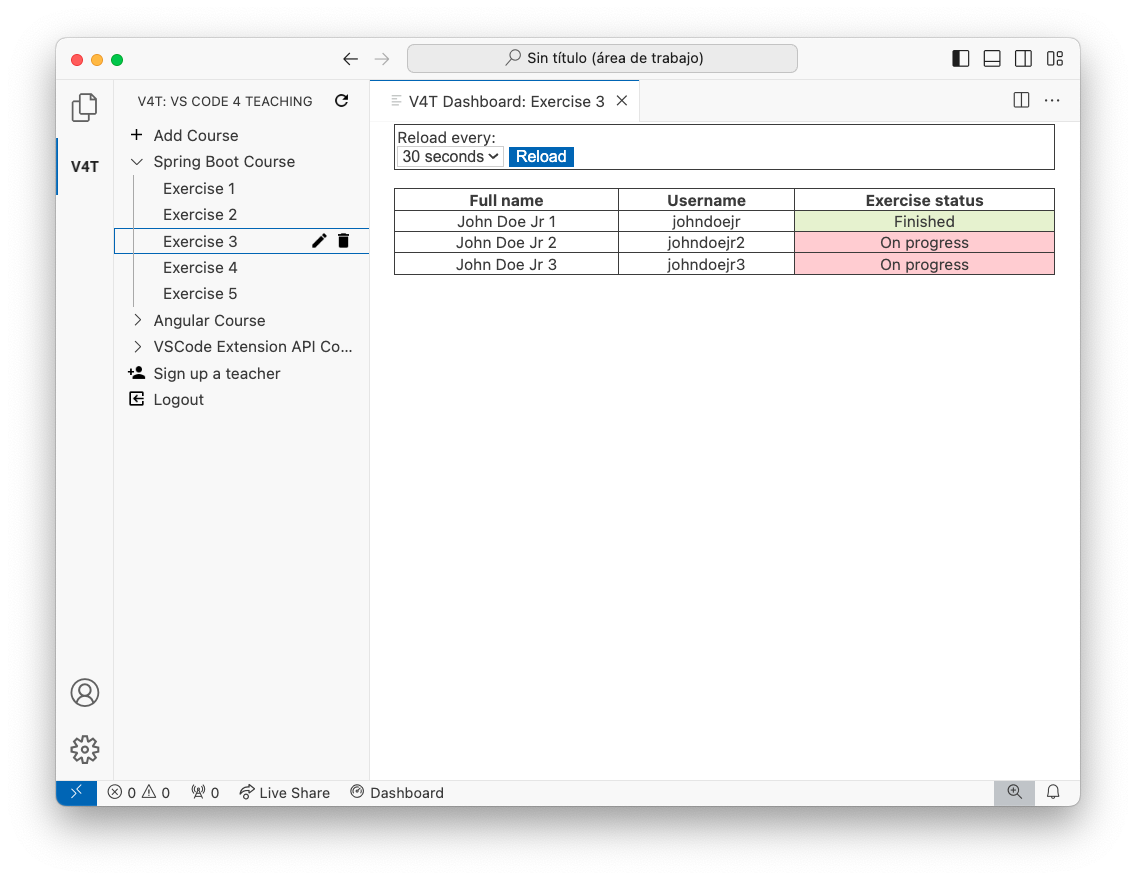
\includegraphics[width=0.825\linewidth]{imagenes/utilizadas/1-introduccion/historia-tfg1-dashboard.png}
    \caption{Captura del \textit{dashboard} para el seguimiento del progreso de los ejercicios en el primer TFG.}
    \label{fig:historiaProyecto1Dashboard}
\end{figure}

\begin{figure}[h!]
    \centering
    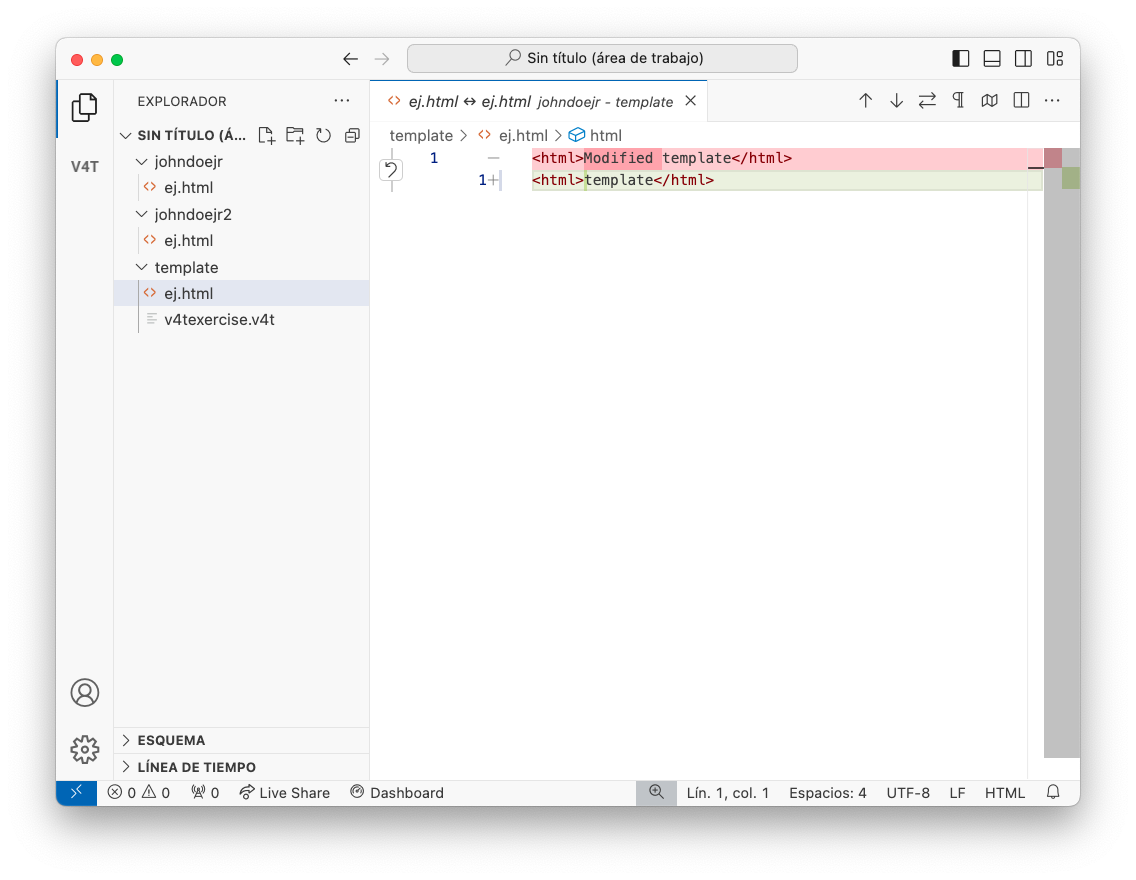
\includegraphics[width=0.825\textwidth]{imagenes/utilizadas/1-introduccion/historia-tfg1-comparacionFicheros.png}
    \caption{Captura de la capacidad para comparación de ficheros en \textit{VSCode4Teaching} en el primer TFG.}
    \label{fig:historiaProyecto1Comparacion}
\end{figure}

Por otro lado, esta primera versión permite a los estudiantes: registrarse en la aplicación, visualizar los cursos en los que están matriculados y sus ejercicios, inscribirse en nuevos cursos utilizando códigos de compartición proporcionados por los profesores, guardar el progreso avanzado durante la realización de los ejercicios y descargar los ejercicios en el punto de progreso en que estuviesen tras la última edición ---o la plantilla en caso de no haberlos comenzado--- y, además, marcar los ejercicios como finalizados para informar al docente, impidiéndose la sincronización de nuevas modificaciones.

Sobre esta base, \textit{VSCode4Teaching} recibió una actualización durante la \textbf{segunda iteración} de su construcción, realizada en el TFG de Álvaro Justo Rivas Alcobendas \cite{TFG_Alvaro}. Durante esta actualización, se buscó potenciar la usabilidad de la herramienta, incorporando numerosas características para, sin modificar reseñablemente el funcionamiento de la aplicación, lograr que todos sus usuarios pudiesen tener una experiencia más completa y mejor informada. Algunas de las mejoras más destacadas son: la incorporación de la actualización en tiempo real del \textit{dashboard} de seguimiento del progreso en la ejecución de ejercicios del que disponen los docentes, que cuenta con mayor cantidad de datos y una apariencia mejorada, tal como se aprecia en la \referenciaFigura{fig:historiaProyecto2Dashboard}; el acceso directo a los ficheros de los estudiantes desde el \textit{dashboard} y la incorporación de una página de ayuda para usuarios ---reflejada en la \referenciaFigura{fig:historiaProyecto2Ayuda}---.

\begin{figure}[ht]
    \centering
    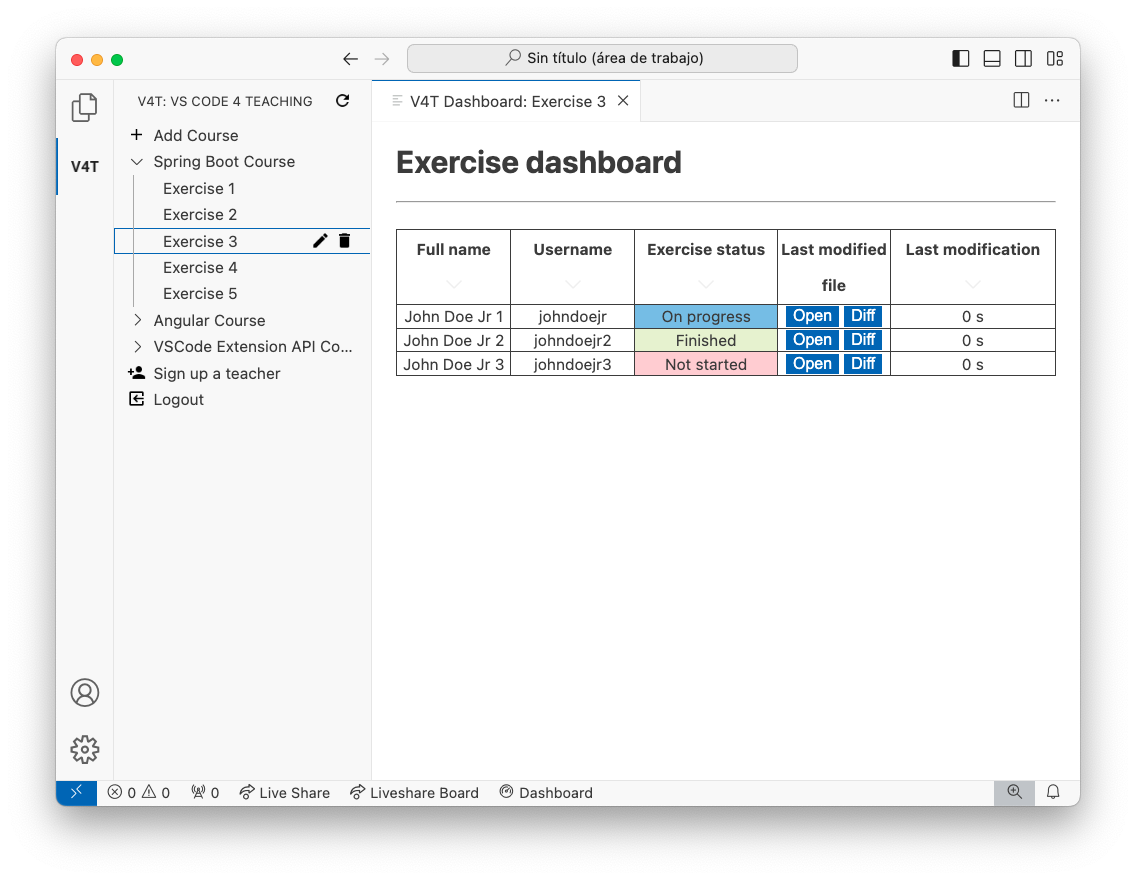
\includegraphics[width=0.825\textwidth]{imagenes/utilizadas/1-introduccion/historia-tfg2-dashboard.png}
    \caption{Captura del \textit{dashboard} para el seguimiento del progreso de los ejercicios en el segundo TFG.}
    \label{fig:historiaProyecto2Dashboard}
\end{figure}

\begin{figure}[ht]
    \centering
    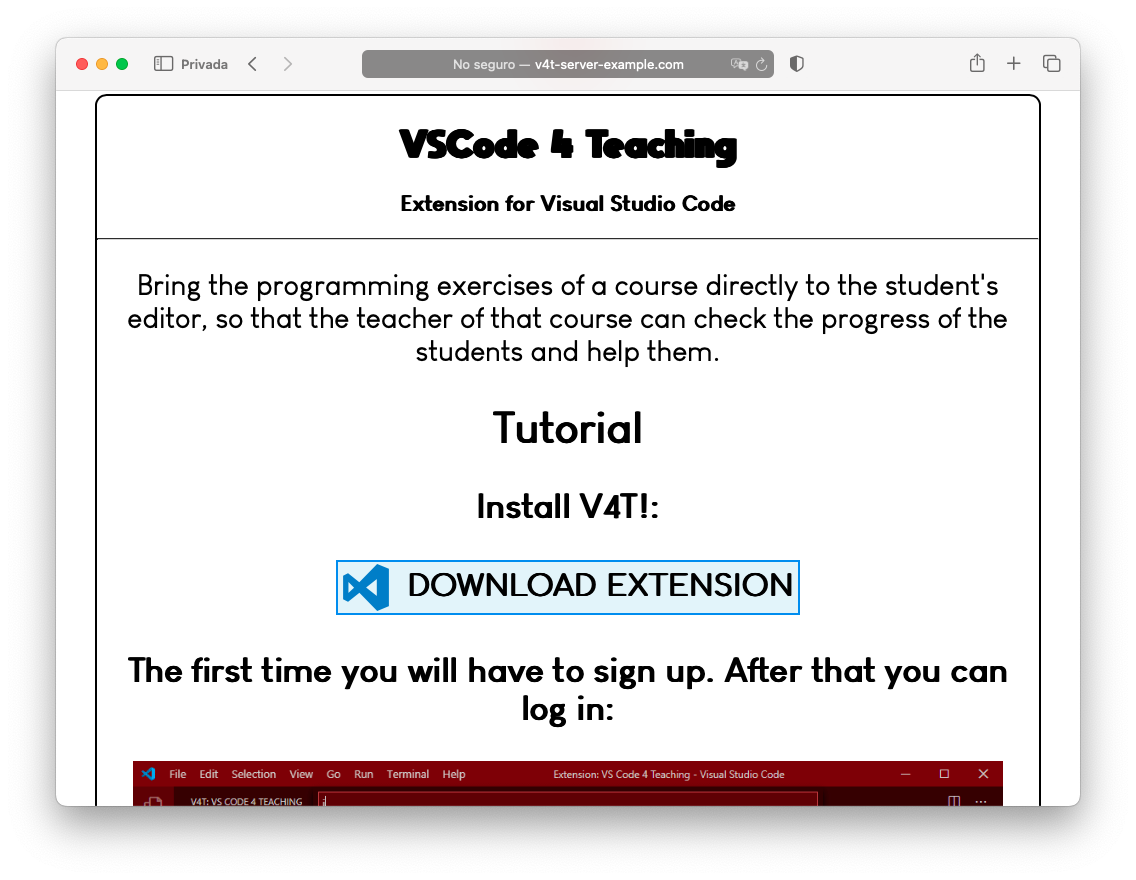
\includegraphics[width=0.825\textwidth]{imagenes/utilizadas/1-introduccion/historia-tfg2-paginaAyuda.png}
    \caption{Captura de la página de ayuda para estudiantes introducida en el segundo TFG.}
    \label{fig:historiaProyecto2Ayuda}
\end{figure}

Una vez explorado el estado inicial del proyecto \textit{VSCode4Teaching} y su funcionalidad disponible, alcanzado mediante las dos evoluciones desarrolladas anteriormente, el presente Trabajo Fin de Grado busca realizar varias tareas enmarcadas esencialmente en el mantenimiento correctivo y perfectivo del proyecto \textit{software} y su funcionalidad, con el fin de alcanzar una tercera evolución de este proyecto para aportarle mayor funcionalidad y calidad. El \referenciaCapitulo{cap:objetivos} detalla el objetivo de este Trabajo Fin de Grado y acota las áreas sobre las que se efectuarán estas mejoras.

\section{Estructura del documento}
El presente documento describe pormenorizadamente cuáles son todas las acciones ejecutadas en materia de evolución y mantenimiento \textit{software} sobre el proyecto en esta tercera iteración de construcción del proyecto \textit{VSCode4Teaching}.

El siguiente apartado (\referenciaCapitulo{cap:objetivos}) recoge los objetivos establecidos en el marco del proyecto que se busca satisfacer en el presente Trabajo Fin de Grado.

El tercer punto (\referenciaCapitulo{cap:tecnolHerramMetodo}) abarca la diversidad de tecnologías y herramientas empleadas para la ejecución del trabajo, así como la metodología de trabajo empleada y la organización para su ejecución.

El apartado cuarto (\referenciaCapitulo{cap:descInformatica}) recoge la descripción informática del trabajo ejecutado. Cabe reseñar que la aplicación queda compuesta por tres grandes componentes: el servidor, la extensión para Visual Studio Code y la aplicación web para navegadores, esta última añadida en el contexto del presente TFG. En torno a cada uno de estos componentes se realiza la descripción de los puntos introducidos en esta sección.

Para finalizar, el capítulo quinto (\referenciaCapitulo{cap:conclusiones}) versa sobre las conclusiones extraídas tras finalizar el desarrollo, analizando la completitud de las necesidades establecidas y estipulando nuevos puntos de mejora para sucesivas iteraciones.

A continuación, una vez finalizado el cuerpo del documento, se introduce la recopilación de referencias bibliográficas a las que aluden las citas introducidas durante el desarrollo del documento.

\noindent\textbf{Nota:} el presente documento contiene diversos enlaces e hipervínculos a páginas web y a otras secciones y epígrafes del documento, destacándolos mediante su introducción en {\color{RedLink}color rojo}. Además, en su edición electrónica, el lector puede hacer \textit{click} sobre estos enlaces para ser conducido al punto al que referencian.




% Sección 2: Objetivos

% 1 página describiendo los objetivos concretos que se pretenden conseguir con el desarrollo del proyecto.
% Es como la conclusión de la introducción y la motivación capítulo anterior.
\afterpage{\blankpage}
\chapter{Objetivos}
\label{cap:objetivos}

\textit{VSCode4Teaching} es, como se ha desarrollado en la \referenciaSeccion{sec:historiaProyecto}, un proyecto ya existente con una amplia funcionalidad disponible para sus usuarios. En ella, los docentes pueden crear cursos con ejercicios de programación basados en plantillas que los alumnos descargarán y sobre las que realizarán sus propuestas de resolución de la problemática planteada, sincronizando su progreso durante su realización, pudiendo así mantener informados en tiempo real a los docentes acerca del progreso de los estudiantes. Durante su construcción y primeros usos, han ido surgiendo de forma progresiva nuevas ideas y requisitos para implementar con el fin de aumentar y mejorar la funcionalidad de la aplicación.

Dada la naturaleza evolutiva y adaptativa de este Trabajo Fin de Grado, el \textbf{principal objetivo} que se marca es alcanzar una evolución del proyecto a través del mantenimiento de su \textit{software}, centrándose en sus vertientes correctiva, implementando soluciones para los errores descubiertos; perfectiva, introduciendo funcionalidad basada en nuevos requisitos y el refinamiento de los actualmente existentes; y preventiva, ejecutando actuaciones para paliar la degradación constante del \textit{software} y conservar su calidad, su eficiencia y su usabilidad.

Tomando como base los puntos de mejora generales existentes en \textit{VSCode4Teaching}, se introduce a continuación la lista de objetivos que se busca ejecutar sobre la herramienta, tanto para crear o refinar funcionalidades y procesos de negocio como para, además, mejorar el propio \textit{software} del proyecto. Estos objetivos, que son el eje vertebrador del Trabajo Fin de Grado, son:

\begin{enumerate}
    \item \underline{Anonimato de los estudiantes}: modificar el sistema de almacenamiento de propuestas de resolución de ejercicios del estudiantado para designarlas de forma anónima, permitiendo al profesorado distinguirlas mediante una relación entre el nombre de cada estudiante y el del directorio anónimo correspondientemente asignado.
    \item \underline{Mejor funcionalidad para docentes}: introducir nuevas funcionalidades para facilitar la interacción de los profesores con la aplicación, como la creación de un nuevo sistema de registro mediante invitación de otros docentes o la incorporación de una característica para que los profesores puedan añadir ejercicios de forma múltiple a sus cursos, entre otros puntos.
    \item \underline{Publicación de propuestas de solución de ejercicios}: aumentar la funcionalidad asociada a los ejercicios, haciendo que puedan albergar una propuesta de solución elaborada por el profesor, permitiéndole añadirla opcionalmente e incorporando los controles pertinentes para poder ajustar su disponibilidad hacia los estudiantes.
    \item \underline{Mejor interfaz de usuario}: potenciar la experiencia de usuario de todos los usuarios poniendo el foco en la obtención de una mejor GUI\footnote{GUI. Siglas de ``interfaz guiada de usuario'' (del inglés \textit{Guided User Interface}). Es el conjunto de elementos gráficos que integran la interfaz empleada por las herramientas informáticas para interactuar bidireccionalmente con los usuarios.} que, mediante nuevos elementos gráficos, facilite el uso de la aplicación, haciéndola más intuitiva y sencilla. Además, con el mismo propósito, incorporar mejoras como la generación de nuevos mecanismos de ayuda personalizados y adecuados a las necesidades específicas de cada alumno y profesor.
    \item \underline{Ciberseguridad}: garantizar el máximo grado de seguridad informática posible para todos los usuarios de \textit{VSCode4Teaching}, introduciendo nuevas políticas de seguridad y manteniendo actualizadas las contramedidas implementadas frente a la aparición de nuevas vulnerabilidades.
    \item \underline{Verificación del \textit{software}}: introducir más pruebas en la aplicación para lograr detectar la mayor cantidad posible de \textit{bugs}\footnote{\textit{Bug}. Es un error producido en el proceso de codificación que provoca incoherencias o fallos en el uso de la aplicación.} o errores presentes en el \textit{software} para, de este modo, proceder a su diagnóstico y corrección.
    \item \underline{Calidad del proyecto y de su \textit{software}}: incorporar mejoras específicamente orientadas a la calidad del \textit{software} y generar una mejor documentación del programa y sus distintos componentes, facilitando así el posterior desarrollo, evolución, mantenimiento y despliegue de la aplicación a otros usuarios y desarrolladores.
\end{enumerate}



% Sección 3: Tecnologías, Herramientas y Metodologías

% Descripción de los lenguajes de programación, entornos de desarrollo, herramientas auxiliares, librerías de
% terceros, sistemas operativos, navegadores web, etc... utilizados para la realización del proyecto así como la
% metodología empleada. El grado de profundidad a la hora de explicar cada tecnología dependerá de lo relevante que
% ha sido para el proyecto y lo conocida que es. Por ejemplo, si se usa el lenguaje de programación Java, no es
% necesario entrar en tanto detalle que si se usa un lenguaje mucho menos usado como Scala, por ejemplo. Respecto
% a la metodología, dada la naturaleza de los proyectos, se suele describir una metodología iterativa e incremental
% en espiral, en la que se van sucediendo reuniones con el profesor que van definiendo el ámbito del proyecto.
% Este capítulo puede tener una extensión entre 10 y 15 páginas.
\chapter{Tecnologías, herramientas y metodología}
\label{cap:tecnolHerramMetodo}
Este capítulo tiene como finalidad la recopilación y presentación de las tecnologías (\referenciaSeccion{sec:tecnologias}), herramientas (\referenciaSeccion{sec:herramientas}) y metodología (\referenciaSeccion{sec:metodologia})
que se han seguido y utilizado para la consecución del presente trabajo.
\section{Tecnologías}
\label{sec:tecnologias}

Se recogen en esta sección las principales tecnologías empleadas para la construcción de \textit{VSCode4Teaching}, dividiéndolas en sendas subsecciones para cada uno de los componentes (al respecto de los componentes, su estructura y sus interrelaciones, véase la \referenciaSeccion{sec:diseñoArquitectura}), e introduciendo, además, información acerca de la persistencia de la información y de las tecnologías involucradas en el despliegue de la aplicación.

\subsection{Persistencia de la información}
Con el fin de almacenar todos los registros para cada una de las entidades del modelo de dominio ---que queda reflejado en la \referenciaSeccion{subsec:arqDominio}---, el servidor hace uso de una base de datos.
Desde el inicio del proyecto, \textit{VSCode4Teaching} ha hecho uso de un sistema gestor de base de datos (SGBD) de tipo relacional, que son aquellos que basan la persistencia de datos en su colocación de tablas que almacenan información estructurada en forma de tuplas (registros) con unos atributos (columnas) comunes a todas.

Específicamente, el SGBD empleado es \textbf{MySQL} \cite{Tec_MySQL}, de Oracle Corporation. Este sistema de tipo relacional es divulgado con licencia pública general de GNU (GPL) en su versión \textit{Community Server}. MySQL es uno de los SGBD más empleados y populares en la actualidad, siendo utilizado por multitud de productos y/o servicios digitales empleados cotidianamente. Este hecho viene ratificado por la \textit{Encuesta de Desarrolladores} realizada por Stack Overflow en 2021 \cite{Tec_Encuesta_StackOverflow}, que confirma en su sección \textit{Most popular technologies: databases} que MySQL es el SGBD más empleado, ya que más del $50 \%$ de los $73\ 317$ encuestados afirman utilizarlo, seguido de cerca por opciones también extendidas como PostgreSQL.

\subsection{Servidor}
\label{subsec:tecServidor}
Esta subsección introduce las tecnologías empleadas para la construcción del servidor que actúa como \textit{backend} de la aplicación, ocupándose principalmente de las tareas de emisión y recepción de información desde y hacia los clientes y de su interpretación para su almacenamiento en el sistema de persistencia de datos.

Con este fin, se hace uso de un componente implementado sobre \textbf{Spring Boot} (basado en el \textit{framework}\footnote{\textit{Framework}. Entorno o marco de trabajo que aglutina una serie de conceptos, prácticas y estándares para facilitar la consecución de un objetivo, como la creación de aplicaciones.} \textbf{Spring}) en lenguaje \textbf{Java}, empleando módulos y dependencias ---gestionadas mediante \textbf{Maven}--- como \textbf{Spring Data}, que hace uso del ORM\footnote{ORM. Siglas de ``mapeador objeto-relacional'' (del inglés \textit{Object-Relational Mapper}). Es una capa de abstracción \textit{software} que permite interactuar con las relaciones, tuplas y atributos de una base de datos a través de los elementos básicos de la orientación a objetos: clases, interfaces, propiedades y métodos.} \textbf{Hibernate} para la gestión de la información en base de datos. Quedan desarrolladas a continuación las tecnologías introducidas anteriormente.

\subsubsection{Java}
Java es ``una plataforma informática de lenguaje de programación creada por Sun Microsystems en 1995'' \cite{Tec_Java}, aunque desde  2010 pertenece a Oracle Corporation tras la integración de Sun Microsystems como filial de la matriz Oracle.

Se puede aseverar que la plataforma Java se basa en la interacción entre tres grandes componentes: el lenguaje Java, el entorno en tiempo de ejecución y el conjunto de las bibliotecas que se proporcionan por defecto.

El lenguaje Java es uno de los más empleados en la industria del \textit{software} (el tercero en noviembre de 2022 según TIOBE \cite{TIOBE}, con una cuota de uso del 11,98\%). Se enmarca dentro del paradigma de la programación orientada a objetos, ya que brinda mecanismos que le permiten verificar sus siete características esenciales ---abstracción, encapsulación, jerarquía, modularización, tipado, concurrencia y persistencia---, entre los que destaca el uso de un tipado fuerte y el soporte a la genericidad, la herencia o el polimorfismo, entre otros.

La plataforma Java dispone, además, de un entorno en tiempo de ejecución, llamado \textit{Java Runtime Environment} (JRE), que es el responsable de la ejecución del código implementado en Java en el computador, gestionando la creación de objetos y la memoria empleada. Este hecho proporciona a Java una de sus principales características: la independencia del sistema operativo o de la plataforma \textit{hardware}. Para ello, hace uso de la máquina virtual de Java, la \textit{Java Virtual Machine} (JVM), que viene incorporada dentro de JRE. Para poder utilizar este entorno de ejecución, Java hace uso de \textit{bytecode}, que es un paso intermedio en la compilación del código que se genera a partir del código fuente y que se convierte a código máquina en el momento en que es utilizado por el entorno de ejecución mediante un compilador JIT (\textit{just in time}), de modo que el lenguaje Java es considerado tanto un lenguaje compilado (ya que se genera el \textit{bytecode} a partir del código fuente, y este es igual en todos los casos) y, además, interpretado (ya que el \textit{bytecode} es procesado por un intérprete en tiempo real durante su ejecución).

Además, la interfaz que Java provee para la utilización de recursos destaca por la ingente cantidad de bibliotecas que introduce, proporcionando una capa de acceso unificado a todo tipo de recursos propios del dispositivo, tales como: la interfaz de red y comunicaciones, el soporte a la concurrencia de procesos ligeros o la gestión de la interfaz gráfica de las aplicaciones, entre muchas otras utilidades.

\subsubsection{Maven}
Maven es un ``\textit{software} de gestión de proyectos y una herramienta basada en el concepto de un modelo de objetos de proyecto (\textit{Project Object Model} o POM) que permite manejar la construcción de proyectos y la generación de informes y documentación a partir de ese fragmento central de información'' \cite{Tec_Maven}.

Maven es un proyecto construido y mantenido por la \textit{Apache Software Foundation} y se divulga de forma abierta bajo licencia Apache. Tal como se introduce en su descripción, Maven es un gestor de dependencias que permite centralizar en un único archivo, el POM (habitualmente \texttt{pom.xml}) en la raíz del proyecto, la declaración de todas las dependencias JAR\footnote{JAR. Acrónimo de \textit{Java ARchive}.} y de todos los \textit{plugins}\footnote{\textit{Plugin}. Es una extensión añadida a un producto informático para aumentar sus capacidades o funcionalidad.} habilitados para su ejecución.

En el \referenciaCodigo{cod:fragmentoPOM} se puede observar un fragmento del fichero POM del servidor de \textit{VSCode4Teaching}. En él se intoducen cuestiones relativas al propio proyecto, tales como el nombre del grupo y del artefacto creados o la versión en que se encuentra; así como datos sobre las dependencias empleadas ---en este caso, declarando que el proyecto se basa en Spring Boot como dependencia principal---. A continuación, quedarán declaradas todas las dependencias, las propiedades y los distintos \textit{plugins} disponibles para ejecutar sobre el proyecto.

\begin{lstlisting}[language=XML,caption={Fragmento del POM del servidor.},label=cod:fragmentoPOM]
<project [...]>
<parent>
    <groupId>org.springframework.boot</groupId>
    <artifactId>spring-boot-starter-parent</artifactId>
    <version>2.7.5</version>
    <relativePath/>
</parent>
<groupId>com.vscode4teaching</groupId>
<artifactId>vscode4teaching-server</artifactId>
<version>2.2.1</version>
<name>VSCode 4 Teaching</name>
<description>Server side of VSCode4Teaching extension.</description>
<properties>
    <java.version>11</java.version>
</properties>
<dependencies>
[...]
\end{lstlisting}

\subsubsection{Spring y Spring Boot}
\label{subsec:spring}
Spring es el \textit{framework} de creación de aplicaciones web basadas en Java más extendido en la industria en la actualidad. Este hecho viene respaldado por la \textit{Encuesta de Desarrolladores} de Stack Overflow \cite{Tec_Encuesta_StackOverflow}, que recoge en su edición de 2021 que, de las $67\ 593$ respuestas de la pregunta \textit{Most popular techonologies: web frameworks}, el $14,56\%$ contestaron que utilizaban Spring por encima de otros, si bien cabe reseñar que ostenta la décima posición en la clasificación general. 

Tal como se describe en su documentación, Spring ``hace que la programación en Java sea más rápida, fácil y segura para todo el mundo [...], poniendo el foco en la velocidad, simplicidad y productividad, convirtiéndolo en el \textit{framework} Java más popular del mundo'' \cite{Tec_Spring}. En la actualidad es filial de la matriz VMWare.

Spring se caracteriza por su modularidad, introduciendo una enorme cantidad de módulos asociados que se pueden utilizar para diversos fines, tales como el trabajo con bases de datos (\textit{Spring Data}), gestión de la seguridad informática (\textit{Spring Security}) o gestión de envío de mensajes (\textit{Spring Integration} o \textit{Web Socket}\footnote{\textit{Web Socket}. Es una tecnología que permite a dos componentes informáticos enviarse mensajes de forma bidireccional a través del protocolo de comunicaciones TCP.}), entre muchos otros.

Spring Boot, en particular, es un proyecto que permite ``facilitar la creación de aplicaciones basadas en Spring preparadas para producción que pueden ejecutarse de forma simple'' \cite{Tec_SpringBoot}.

Spring y Spring Boot vienen siendo empleados en el presente proyecto desde su comienzo por cuatro factores: la facilidad con la que permite crear un servidor web para exponer la API\footnote{API. Siglas de ``interfaz de programación de aplicaciones'' (del inglés \textit{Application Programming Interface}). Es un componente \textit{software} destinado a las comunicaciones entre el sistema que la incorpora y otros sistemas que se comunican con este.} REST\footnote{REST. Siglas de ``transferencia de estado representacional'' (del inglés \textit{Representational State Transfer}). Es un estilo empleado para la transmisión de información en sistemas distribuidos.} \footnote{API REST. Es un conjunto de \textit{endpoints} que se basa en el estilo REST para intercambiar información entre un servidor y uno o más consumidores o clientes.} desarrollada, la facilidad para la gestión de las dependencias (mediante Maven) y la persistencia de la información (mediante el ORM Hibernate), la capacidad de utilizar módulos de Spring como \textit{Spring Data} o \textit{Spring Security} en el proyecto y la simplificación del despliegue del servidor (a partir del uso de Spring Boot).

\subsubsection{JUnit}
JUnit es la principal librería para la implementación y ejecución de pruebas o \textit{tests}\footnote{\textit{Test}. Es una prueba realizada sobre una pieza de \textit{software} para garantizar que su comportamiento real es congruente con el deseado.} para la verificación del \textit{software} en entornos Java \cite{Tec_JUnit}.
Esta plataforma, que fue originalmente creada por Kent Beck y Erich Gamma, se distribuye bajo licencia Eclipse Public License y es de uso público y gratuito.

JUnit permite a los desarrolladores la ejecución controlada de pruebas implementadas en código basadas en aserciones. Introduce múltiples características para dar soporte a pruebas parametrizadas y a dobles\footnote{Doble. En el ámbito de las pruebas codificadas o \textit{tests}, es una pieza de código que permite reemplazar el comportamiento de objetos de producción o dependencias en el momento de ejecutar las pruebas.}. Destaca, además, por su fácil utilización en sistemas de integración continua y en los principales entornos de desarrollo al contar con una incorporación sencilla en proyectos Java gestionados mediante Maven.

\subsection{Extensión para Visual Studio Code}
\label{subsec:tecCliente}
La presente subsección recoge un resumen de las principales tecnologías empleadas para la generación de la extensión para Visual Studio Code que emplean los usuarios finales descargándola y ejecutándola en sus instancias locales del mencionado IDE\footnote{IDE. Siglas de ``entorno de desarrollo integrado'' (del inglés \textit{Integrated Development Environment})}.

Esta extensión se basa en la utilización de la \textbf{Visual Studio Code Extension API} para su construcción. Tanto Visual Studio Code como sus extensiones hacen uso de \textbf{Node} como plataforma para la ejecución de código. Además, se hace uso de \textbf{TypeScript} para obtener un código más robusto y organizado, y de \textbf{Jest} para la ejecución de pruebas. Se desarrollan en sendas subsecciones posteriores cada una de las mencionadas tecnologías.

\subsubsection{Node}
Node.js (habitualmente denominado ``Node'') es un ``entorno de ejecución para JavaScript construido con V8\footnote{V8. Es el motor de JavaScript que utiliza el navegador Google Chrome para la ejecución de los \textit{scripts}, empleado también para la ejecución de aplicaciones de escritorio implementadas utilizando este lenguaje.}'' \cite{Tec_Node}; esto es, es una plataforma que permite la ejecución de programas basados en el lenguaje JavaScript, permitiendo construir todo tipo de \textit{software}.

JavaScript es, según el índice TIOBE \cite{TIOBE}, el séptimo lenguaje de programación más empleado, con una cuota de uso cercana al 2,74\% en noviembre de 2022. Las finalidades tradicionales de este lenguaje lo ceñían a una utilización meramente enfocada en el aporte de dinamismo a las aplicaciones web ejecutadas en el navegador. Sobre esta base, Node busca abstraer la funcionalidad de este lenguaje para conducirla a la generación de aplicaciones de escritorio.

Una de las principales características de Node ---y la causante principal de su creación original--- es la necesidad de trasladar el modelo de ejecución propio de la plataforma JavaScript, basado en eventos asíncronos, a la creación de aplicaciones con gran dependencia de conexiones por red avanzadas. Las grandes capacidades de Node han derivado paulatinamente en la creación de \textit{frameworks} para la generación de aplicaciones web de tipo SPA\footnote{SPA. Siglas de ``aplicación de página única'' (del inglés \textit{Single Page Application}). Típicamente, las aplicaciones web SPA son aquellas que ejecutan toda su funcionalidad en una sola página, para lo que se basan en intercambios de información en segundo plano con el servidor y modificaciones en la interfaz de usuario.} que se construyen para ser ejecutadas en el navegador y que, ya que se deben construir sobre la plataforma JavaScript, basan sus procesos de ejecución, compilación o verificación en Node. Un ejemplo es Angular, que se ha utilizado en este Trabajo Fin de Grado para generar un nuevo componente, tal como queda desarrollado en la \referenciaSeccion{subsec:tecAppWeb}.

Node introduce por defecto en sus proyectos NPM (en inglés, \textit{Node Package Manager}), que es el ``registro de \textit{software} más grande del mundo, siendo empleado por desarrolladores de código abierto de todos los continentes para compartir y prestar sus paquetes'' \cite{Tec_NPM}. NPM se basa en el uso de un fichero, \textit{package.json}\footnote{JSON. Siglas de ``notación de objetos de JavaScript'' (del inglés \textit{JSON Object Notation}). Es un formato para la escritura de datos basado en la sintaxis de los objetos en el lenguaje \textit{JavaScript} muy empleado por su fácil comprensión y gran versatilidad.}, contenido en la raíz de los proyectos Node. Este fichero introduce declaraciones sobre el propio proyecto ---tales como su nombre, autoría o licencia--- y sobre las dependencias que emplea.
En el \referenciaCodigo{cod:fragmentoPackageJSON} se observa, a título de ejemplo, un fragmento del fichero \textit{package.json} de la extensión para Visual Studio Code de \textit{VSCode4Teaching}, incluyendo el nombre, la versión y las dependencias empleadas, entre muchos otros datos.

\begin{lstlisting}[language=JavaScript,caption={Fragmento del \textit{package.json} de la extensión de \textit{VSCode4Teaching}.}, label=cod:fragmentoPackageJSON]
{
"name": "vscode4teaching",
"publisher": "VSCode4Teaching",
// [...],
"description": "Bring the programming exercises directly to the student's editor.",
"version": "2.2.1",
// [...],
"dependencies": {
    "axios": "^1.1.3",
    "form-data": "^4.0.0",
    // [...]
},
// [...]
}
\end{lstlisting}

\subsubsection{TypeScript}
TypeScript es ``un lenguaje fuertemente tipado que compila a JavaScript, proporcionando mejores herramientas a todos los niveles'' \cite{Tec_TS}. Ha sido creado y es actualmente mantenido por Microsoft y se divulga mediante licencia Apache de código abierto. El lenguaje TypeScript permite la utilización de tipos en ficheros de código fuente que pueden ser compilados a ficheros de código en JavaScript, siendo esta su característica más destacada y diferenciadora.

La utilización de TypeScript permite, por tanto, conseguir trasladar las ventajas derivadas de la utilización de lenguajes fuertemente tipados, tales como una programación segura en cuanto a los tipos de las variables ---impidiendo errores de tipos--- al código fuente que finalmente se transpilará a código válido en JavaScript, facilitando la refactorización del código y permitiendo generar, indirectamente, una mejor documentación del código.

\subsubsection{Visual Studio Code Extension API}
Visual Studio Code es el entorno de desarrollo integrado para el que se construye la extensión de \textit{VSCode4Teaching} (ver \referenciaSeccion{subsec:edicionCodigo} al respecto). Este entorno de desarrollo tiene como uno de sus pilares esenciales la ``extensibilidad'' \cite{Tec_VSCodeExtAPI}, de modo que su funcionalidad puede ser expandida haciendo uso de extensiones disponibles a través del \textit{Marketplace} (del inglés, ``mercado'') \cite{Tec_VSCPublish}.

Como consecuencia, los creadores de Visual Studio Code ponen a disposición de la comunidad de desarrolladores una API que les permite implementar, construir y publicar extensiones ejecutables dentro del editor de código, proporcionando una interfaz que hace que las extensiones tengan acceso a prácticamente la totalidad de la funcionalidad básica del IDE. Así, las extensiones pueden introducir nuevos comandos en el entorno de desarrollo, añadir la capacidad de incorporar comentarios textuales acerca del código, modificar el entorno del editor, añadir funcionalidad para la depuración de código y acceder al control de las ventanas y las áreas de trabajo activas.

\subsubsection{Jest}
Jest es una herramienta para la introducción de pruebas (\textit{tests}) en aplicaciones basadas en JavaScript que ``pone el foco en la simplicidad'' \cite{Tec_Jest}. Es una plataforma creada originalmente por Facebook, actualmente mantenida por la \textit{Open JS Foundation} y distribuida bajo licencia MIT como código abierto.

En línea con otras utilidades para la realización de pruebas, introduce mecanismos como las aserciones o los dobles, ofreciendo una interfaz por línea de comandos muy sencilla de utilizar para los desarrolladores. Además, esta característica permite su fácil integración con el mecanismo de gestión de dependencias NPM.

Este es el \textit{framework} de creación y ejecución de pruebas elegido para la extensión desarrollada desde el comienzo del proyecto, habiéndola escogido por la gran funcionalidad que ofrece frente a otros \textit{frameworks} y el buen soporte del que dispone a través de su documentación y su comunidad de usuarios.

\subsection{Aplicación web: Angular}
\label{subsec:tecAppWeb}
En el contexto del trabajo abordado en el presente documento, se ha llevado a cabo la introducción de una aplicación web que actúa como cliente para la expansión de funcionalidad de \textit{VSCode4Teaching} (ver \referenciaSeccion{sec:diseñoArquitectura} al respecto).

Para crear e implementar la aplicación web, se ha decidido hacer uso de \textbf{Angular}, que es un \textit{framework} de código abierto distribuido bajo licencia MIT y originalmente creado por Google que permite la creación de \textbf{aplicaciones web SPA}.

Las aplicaciones web SPA o de una sola página son aquellas en las que todas las pantallas son mostradas en una misma página que modifica su contenido de forma dinámica según la interacción que realice el usuario. La utilización de las aplicaciones web SPA ha crecido en popularidad en los últimos años, ya que permite obtener una mejor experiencia de usuario al cargar una menor cantidad de recursos cada vez que este interactúa con la página, convirtiéndose en el tipo de aplicación ideal para utilidades como gestión, administración o paneles de control, entre muchos otros fines.

El auge y crecimiento del uso de este tipo de aplicaciones ha potenciado la aparición de numerosos \textit{frameworks} que permiten simplificar su creación y desarrollo, tales como Vue \cite{Tec_Vue}, React \cite{Tec_React} o Angular \cite{Tec_Angular}.

En el caso de este proyecto, se ha decidido utilizar Angular atendiendo fundamentalmente a dos factores: funciona sobre las mismas plataformas que la extensión para Visual Studio Code ---lenguaje TypeScript y proyecto Node---, facilitando así la curva de aprendizaje para desarrolladores de este proyecto; y es el \textit{framework} que se estudia durante el Grado en Ingeniería del \textit{Software} en la Universidad Rey Juan Carlos, facilitando así su posterior mantenimiento.

\subsection{Distribución y despliegue}
\label{subsec:tecDistribDespliegue}
La distribución y el despliegue de \textit{VSCode4Teaching} involucran el uso de diversas tecnologías. Una de las formas disponibles más sencillas para el despliegue del servidor ---junto con la aplicación web--- es hacer uso de la configuración suministrada para la compilación de una imagen \textbf{Docker}. Las tecnologías descritas en esta sección se ven complementadas por el uso de herramientas que facilitan el despliegue, como el sistema de integración, despliegue y entrega continuas (ver \referenciaSeccion{subsec:cicd}). Se desarrolla en profundidad la información acerca del desliegue en la \referenciaSeccion{sec:distribDespliegue}.

\subsubsection{Docker}
Docker es ``una plataforma diseñada para ayudar a los desarrolladores a construir, compartir y ejecutar aplicaciones modernas'' \cite{Tec_Docker} que se basa en el uso de contenedores, que son ``unidades estandarizadas y ligeras de \textit{software} preparadas para el desarrollo y despliegue [...] que agrupan el código y todas sus dependencias para ejecutar aplicaciones rápida y fiablemente proporcionando beneficios similares a la virtualización (como, por ejemplo, el aislamiento de las aplicaciones sobre el resto del computador) pero sin sacrificar la eficiencia, ya que se ejecutan sobre un sistema operativo ---y no directamente sobre \textit{hardware}---'' \cite{Tec_DockerContainers}.

Alrededor de Docker existen numerosas tecnologías con todo tipo de propósitos, siendo una de las más destacadas \textbf{Docker Compose}. Docker Compose es una ``herramienta que permite definir y ejecutar aplicaciones de Docker multicontenedor'' \cite{Tec_DockerCompose}; esto es, que requieren de la ejecución simultánea de más de un contenedor de herramientas diferentes ---por ejemplo, una aplicación Java y un servidor de bases de datos MySQL---.

\section{Herramientas}
\label{sec:herramientas}

Se recogen en esta sección, por otro lado, las principales herramientas empleadas durante el proceso \textit{software} ejecutado para la realización del presente TFG. El uso de estas herramientas tiene, en todos los casos, la finalidad de mejorar el rendimiento del proceso favoreciendo una mejor organización o introduciendo facilidades para el desarrollo \textit{software}.

\subsection{Herramientas para el producto}
\subsubsection{Edición de código}
\label{subsec:edicionCodigo}
Habitualmente, la edición del código se realiza en entornos de desarrollo integrados (IDE), que son aplicaciones que incluyen una ingente cantidad de utilidades y servicios que permiten a los desarrolladores la redacción del código de una forma más sencilla, facilitando así el proceso de desarrollo.

Por la naturaleza de los tres componentes que forman \textit{VSCode4Teaching} en la actualidad ---detallada en la \referenciaSeccion{sec:diseñoArquitectura}---, se han utilizado tres entornos diferentes.

\textbf{Visual Studio Code} \cite{Her_VSCode}, de Microsoft (distribuido bajo licencia MIT), ha sido el IDE más empleado durante el proceso de desarrollo, ya que uno de los componentes de la aplicación es una extensión para este IDE.

Por otro lado, \textbf{IntelliJ IDEA} \cite{Her_IntelliJ}, de JetBrains (gratuito para fines eduativos), ha sido el IDE empleado para el desarrollo del servidor, ya que es un entorno enfocado a la creación y confección de proyectos Java y, específicamente, de aplicaciones web basadas en Spring.

A estas herramientas se suma \textbf{WebStorm} \cite{Her_WebStorm}, un entorno de JetBrains hermano de IntelliJ IDEA destinado específicamente a la plataforma JavaScript y con soporte, además, para el lenguaje TypeScript. También es gratuito para fines eduativos, y ha sido el IDE empleado para el desarrollo de la aplicación web SPA.

\subsubsection{Visualización de base de datos}
De entre la ingente cantidad de herramientas que existen para la gestión gráfica de bases de datos MySQL, la empleada durante este TFG ha sido \textbf{DBeaver} \cite{Her_DBeaver}. Es una aplicación gratuita multiplataforma ---distribuida con licencia Apache 2.0--- orientada a desarrolladores y administradores de bases de datos y que soporta todos los SGBD relacionales más populares, entre los que se encuentra el empleado en este proyecto.

\subsubsection{Sistema de control de versiones}
\label{subsec:vcs}
Los sistemas de control de versiones permiten a los equipos de desarrollo obtener un seguimiento de las distintos cambios ejecutados sobre un proyecto, añadiendo diversas opciones para la gestión de solapamientos o conflictos y para la diversificación del desarrollo en distintas tareas realizables simultáneamente mediante el concepto de ``rama'' de desarrollo.

Uno de los más extendidos en la actualidad es \textbf{git}, que es un ``sistema de control de versiones distribuido, gratuito y de código abierto diseñado para manejar con velocidad y eficiencia desde proyectos pequeños hasta muy grandes'' \cite{Her_Git} que, además, se distribuye bajo licencia GNU 2.0 (siendo, por tanto, \textit{software} libre).

En particular, para la ejecución de este proyecto se ha utilizado un repositorio público alojado en \textbf{GitHub}, que es un servicio que añade a git capacidades adicionales mediante una interfaz gráfica intuitiva y fácil de utilizar. Es empleada por más de 83 millones de desarrolladores y en ella hay registrados más de 200 millones de repositorios, haciendo de ella ``la plataforma de desarrollo más grande del mundo en la actualidad'' \cite{Her_GitHub}.

La \referenciaSeccion{sec:distribDespliegue} introduce más detalles acerca de la distribución del código del proyecto \textit{VSCode4Teaching}.

\subsubsection{CI/CD}
\label{subsec:cicd}
CI/CD es la abreviatura de \textit{Continuous Integration/Continuous Deployment}, traducido del inglés como ``integración continua/despliegue continuo'' (o, en ocasiones, ``integración continua/entrega continua''). Es uno de los procesos incluidos en la filosofía \textit{DevOps}, que está conformada por ``un conjunto de prácticas, herramientas [...] que sirve para automatizar e integrar los procesos [...] del equipo de desarrollo y de tecnologías de la información'' \cite{Her_DevOps}.

Así, CI/CD permite ``automatizar el flujo de desarrollo del \textit{software} para desplegar código de mejor calidad con mayor frecuencia usando un proceso iterativo y continuo para compilar, probar y desplegar, previniendo la posterior aparición de errores y fallos en el código'' \cite{Her_CICD}.

En el caso de este proyecto se hace uso de la herramienta \textbf{Travis CI}, que es una plataforma que permite ``compilar, probar y desplegar el código fácil y rápidamente'' \cite{Her_Travis} y que es gratuita para proyectos de \textit{software} libre, tal como lo es \textit{VSCode4Teaching}.
Para ello, se introduce un fichero llamado \texttt{.travis-ci.yml} en la raíz del proyecto. Este contiene la información que permite compilar y desplegar la imagen Docker, divulgándola a través de Internet. En el \referenciaCodigo{cod:travis} se introduce una parte del mencionado fichero como muestra de ejemplo de la configuración para el uso de Travis CI.

\begin{lstlisting}[language=YAML,caption={Fragmento del fichero de configuración de Travis CI para desplegar y divulgar la versión 2.2.0 de \textit{VSCode4Teaching}.},label=cod:travis]
jobs:
    include:
        - name: V4T Server (Spring Boot)
            jdk: oraclejdk11
            [...]
            script:
                - "./mvnw clean package -B -q"
            after_script:
                - docker build -t vscode4teaching/vscode4teaching:2.2.0 .
                - docker build -t vscode4teaching/vscode4teaching:latest .
                - docker push vscode4teaching/vscode4teaching:2.2.0
                - docker push vscode4teaching/vscode4teaching:latest
        - name: V4T Extension (Node.js)
            node_js: 10.15.3
            [...]
            before_script:
                - cd ./vscode4teaching-extension
                - npm install --save-dev
            script:
                - npm test
[...]
\end{lstlisting}

\subsection{Organización del proceso: Trello}
\label{subsec:herTrello}
Se ha realizado el presente Trabajo Fin de Grado siguiendo un proceso \textit{software} de pequeñas iteraciones que queda detallado en la \referenciaSeccion{sec:metodologia}. Tal como se recoge en la citada sección, uno de los principios básicos seguidos para la organización del trabajo ha sido la utilización de un tablero de tipo Kanban para la visualización, división, distribución y jerarquía de las tareas.

Durante el transcurso del proceso, \textbf{Trello} ha sido la herramienta informática empleada para ejecutar esta organización. Trello es una plataforma de uso gratuito de Atlassian que permite ``gestionar proyectos y lograr cotas más altas de productividad independientemente de la dinámica de trabajo'' \cite{Her_Trello}.

\begin{figure}[h]
    \centering
    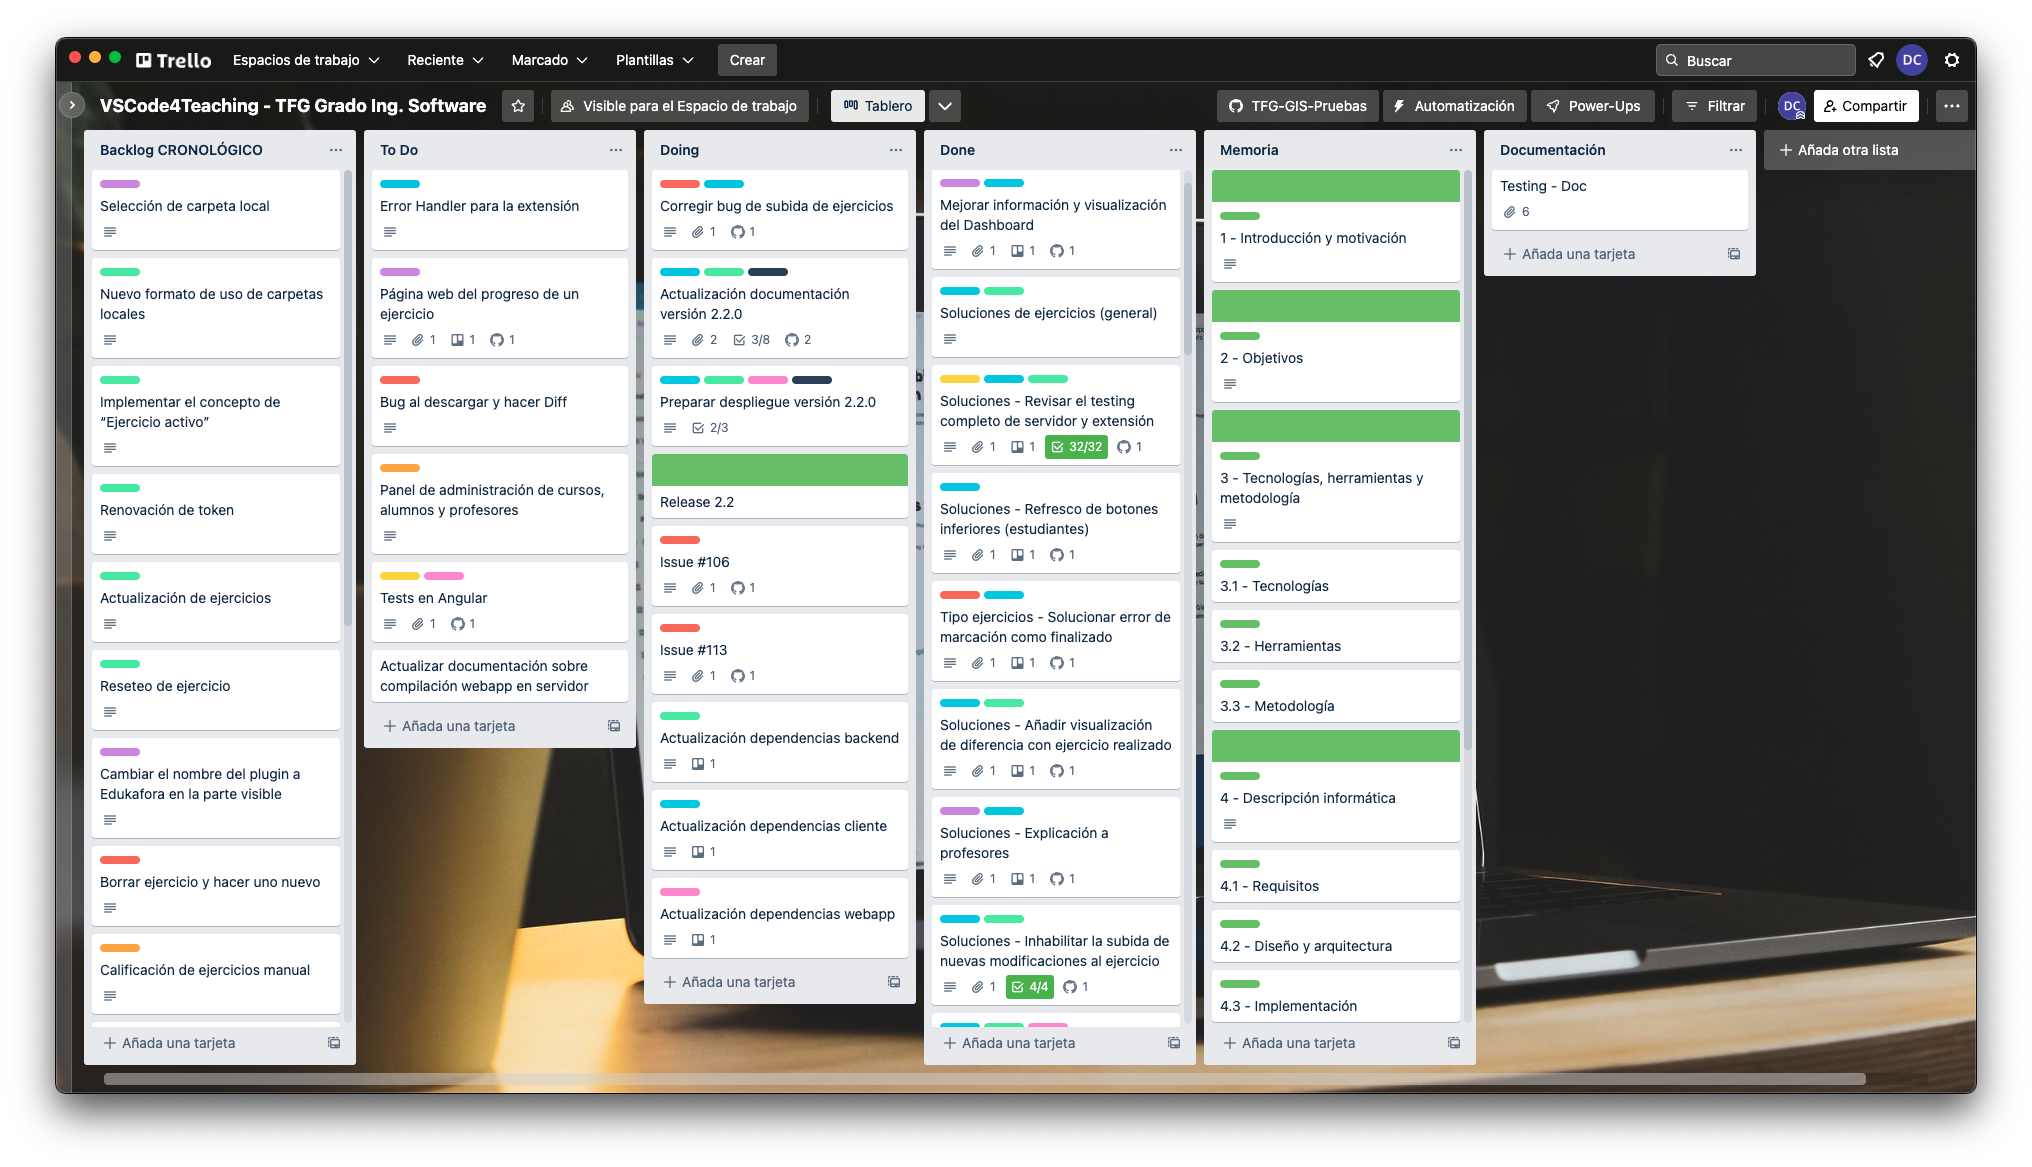
\includegraphics[width=\textwidth]{imagenes/utilizadas/3-2-herramientas/capturaTrello.png}
    \caption{Captura del tablero de trabajo Trello empleado.}
    \label{fig:Trello}
\end{figure}

La \referenciaFigura{fig:Trello} permite visualizar una captura del tablero empleado en Trello.
Esta herramienta permite la creación de diversas tarjetas representativas de tareas distribuidas en varias columnas a las que se les puede asignar fechas de inicio y finalización, así como etiquetas de distintos colores para su distinción temática, pudiendo además añadir comentarios y recursos adicionales ---hipervínculos, documentos adjuntos o enlaces hacia otras tarjetas asociadas, por ejemplo---. Mediante todas estas funcionalidades, esta herramienta permite a sus usuarios organizar de forma sencilla, intuitiva y muy visual el trabajo pendiente y realizado, facilitando la toma de decisiones de diseño y desarrollo y aumentando la productividad del tiempo dedicado.

Esta explicación queda ampliada en la \referenciaSeccion{sec:metodologia}, que aborda la forma de utilización del tablero Trello y su integración en el proceso de desarrollo seguido.

\section{Metodología: proceso \textit{software}}
\label{sec:metodologia}

En el ámbito de la ingeniería informática ---y, particularmente, en la ingeniería del \textit{software}---, existe una gran variedad de técnicas, metodologías y \textit{frameworks} que permiten a los equipos de desarrollo organizarse de forma correcta, dividir adecuadamente la carga de trabajo pendiente y planificar temporalmente los hitos a cumplir para alcanzar un método de funcionamiento que optimice al máximo la productividad.

Muestra de ello son los conocidos como ``\textit{frameworks} ágiles'' (del inglés, \textit{agile}), que son un conjunto de metodologías y formas de proceder que destacan por la importancia que otorgan al factor humano, a la capacidad de respuesta frente al cambio o a la colaboración constante con el destinatario o el adquiriente del \textit{software} desarrollado, tal como se detalla en el \textit{Manifiesto Ágil} \cite{Met_AgileManifesto}. Algunos de los \textit{frameworks} ágiles más populares en la actualidad son \textit{Kanban}, \textit{Scrum} o \textit{eXtreme Programming} (XP) \cite{Met_AgileFrameworks}, entre otros.

Sin embargo, estos procesos \textit{software} están concebidos para ser aplicados en grupos de trabajo formados por múltiples integrantes, por lo que no tiene cabida la aplicación directa y fidedigna de sus herramientas en proyectos de un solo autor, como es el caso del presente Trabajo Fin de Grado. Sin embargo, esto no es óbice para poder tomar algunas de las técnicas que introducen y adaptarlas para su utilización y que, de ese modo, poder articular un proceso \textit{software} adecuado para el contexto concreto del presente Trabajo.

El proceso de desarrollo ejecutado toma como pilar esencial uno de los puntos principales de la filosofía ágil: desarrollo iterativo e incremental basado en la consecución de pequeñas iteraciones completas, introduciendo en cada una de estas todos los puntos esenciales que forman parte de los procesos de desarrollo \textit{software}: especificación de  requisitos, diseño y planteamiento de la solución, implementación en código y verificación o \textit{testing}, alcanzando cada uno de ellos la duración temporal requerida para garantizar la completitud de la ejecución del proceso. En el tiempo empleado para completar el Trabajo Fin de Grado se han llevado a cabo un total de 52 iteraciones.

Antes de comenzar el proceso de desarrollo, dada la existencia previa de \textit{software} funcional sobre el que continuar trabajando para la consecución de los objetivos estipulados, fue necesario comenzar con un periodo de aprendizaje y asimilación de la arquitectura de \textit{VSCode4Teaching} y las tecnologías que lo conforman, iniciando la implementación de algunas tareas más sencillas en paralelo y avanzando paulatinamente hacia la ejecución de tareas más complejas a medida que evolucionaba el conocimiento y aprendizaje acerca del proyecto en su completitud.

No obstante, cabe reseñar que no todas las iteraciones realizadas durante el presente proyecto han tenido como finalidad la implementación específica de mejoras o nuevas funcionalidades, sino que algunas de las iteraciones previamente citadas han sido dedicadas a otros tipos de tareas. A este respecto, un ejemplo reseñable son las iteraciones dedicadas a la garantía de seguridad informática, actualizando las dependencias y bibliotecas empleadas en cada uno de los componentes de la aplicación para utilizar versiones revisadas frente a vulnerabilidades de reciente aparición, garantizando así la ausencia de riesgos de seguridad en el \textit{software} desarrollado y ejerciendo un mantenimiento preventivo sobre el proyecto.

Otro caso paradigmático de este hecho son las iteraciones centradas en la corrección de errores o \textit{bugs} detectados y registrados en paralelo al proceso habitual de desarrollo o en pruebas de simulación de entornos reales ---ver \referenciaSeccion{subsec:pruebasManuales}---. En estos casos, se ha seguido un proceso cíclico de tres fases: triaje del error, obteniendo la respuesta a cómo, cuándo, dónde y por qué se produce el error, acotando así su contexto; implementación de la solución, ejecutando las acciones pertinentes sobre el código para solucionar el fallo analizado; y verificación de la solución, comprobando si se sigue produciendo el error y, en caso de ser así, volviendo a ejecutar el proceso íntegro sobre él de nuevo hasta subsanarlo.

La metodología empleada durante este Trabajo Fin de Grado se ha visto soportada en el uso de diversas herramientas de ayuda a la organización de trabajos en materia de programación informática. De este modo, se han empleado recursos como un sistema de control de versiones git o un tablero Kanban en Trello, tal como queda explicado en la \referenciaSeccion{sec:herramientas}.

El tablero de Trello se ha utilizado de la misma forma en que se emplea en la metodología ágil Kanban \cite{Met_TableroKanban}, estructurándolo en las siguientes columnas: \textit{backlog}, que contiene todas las tarjetas pendientes de planificación; \textit{to do}, que incluye todas las tareas que se encuentran inminentes a su comienzo; \textit{doing}, que contiene las tarjetas que se están realizando en el momento de observar el tablero; y \textit{done}, que alberga las tarjetas ya finalizadas en orden de ejecución. De este modo, estos ítems se desplazan entre las columnas anteriormente detalladas consecutivamente y en orden, convirtiendo las tarjetas del \textit{backlog} en tareas atómicas al acceder a \textit{to do}, trasladándolas a \textit{doing} en el momento de comenzar su implementación; y desplazándolas finalmente a \textit{done} una vez finalizada su implementación.


% Sección 4: Descripción informática

% Descripción del proyecto realizado.
% Después de unos párrafos introductorios el capítulo se divide en subcapítulos.
% Extensión recomendada: de 25 a 35 páginas.
\afterpage{\blankpage}
\chapter{Descripción informática}
\label{cap:descInformatica}
Esta sección incluye información pormenorizada acerca del proceso de desarrollo informático ejecutado para la consecución de los objetivos estipulados en el \referenciaCapitulo{cap:objetivos}.
Esta descripción se realiza siguiendo el orden típico de los procesos \textit{software}, introduciendo una enumeración de los requisitos establecidos (\referenciaSeccion{sec:requisitos}), la descripción de las modificaciones en el diseño y la arquitectura de los distintos componentes involucrados (\referenciaSeccion{sec:diseñoArquitectura}), el detalle acerca de la implementación de los requisitos introducidos (\referenciaSeccion{sec:implementacion}), la verificación del \textit{software} y de su calidad (\referenciaSeccion{sec:verificacion}) y su distribución y despliegue (\referenciaSeccion{sec:distribDespliegue}).

% Sección 4.1: Requisitos.
% Descripción detallada de las funcionalidades que tendría que implementar la aplicación (pues se asume que los
% requisitos se escriben antes de empezar el desarrollo). Pueden tener forma de historias de usuario o bien ser una
% lista de requisitos funcionales y no funcionales.
\section{Extracción de requisitos}
\label{sec:requisitos}

A partir de los objetivos iniciales establecidos en el \referenciaCapitulo{cap:objetivos}, se procede a extraer una lista de requisitos que especifique de forma corta, clara y concisa las tareas atómicas que se ejecutarán durante el proceso de implementación para la consecución de los citados objetivos. Estos requisitos quedan divididos en tres categorías: requisitos funcionales, no funcionales y de corrección de errores.
Se antepone a cada uno un identificador del aspecto \texttt{RX-Y}, donde \texttt X puede ser ``F'' (para los requisitos funcionales), ``N'' (no funcionales) o ``E'' (corrección de errores); e \texttt Y es un valor numérico correlativo. Estos identificadores serán empleados durante el resto del documento para referenciar a sus requisitos asociados.

Se recogen a continuación todos los requisitos que han tenido una consecución satisfactoria en el contexto del presente Trabajo Fin de Grado.

\subsection{Requisitos funcionales}
\label{subsec:listaReqsFuncionales}
Esta categoría abarca todos los requisitos destinados a los usuarios finales; esto es, los conducentes a la mejora de la funcionalidad disponible en la aplicación y que, por tanto, se llevan a cabo mediante la introducción de nuevas funciones o el mantenimiento de capacidades previamente existentes en el \textit{software}. Estos requisitos quedan redactados como ``historias de usuario'' ---práctica extraída de eXtreme Programming (XP)--- \cite{XP_UserStories}, plasmándolos así en un formato más sencillo y fácil de entender que sitúa la necesidad del usuario final en un papel de máxima relevancia. Estos son:
\begin{itemize}
    \item \texttt{\textbf{RF-1}}: como profesor, quiero poder invitar a nuevos docentes para así hacer llegar \textit{VSCode4Teaching} a otros profesores.
    \item \texttt{\textbf{RF-2}}: como profesor, quiero poder añadir ejercicios a mis cursos de forma masiva para mejorar mi eficiencia.
    \item \texttt{\textbf{RF-3.1}}: como profesor, quiero poder visualizar de forma anónima las soluciones de los alumnos a los ejercicios para poder mostrarlas en el aula sin vulnerar el anonimato de sus autores.
    \item \texttt{\textbf{RF-3.2}}: como profesor, quiero poder disponer de la capacidad para ocultar y mostrar los nombres de los alumnos en el \textit{dashboard} para así poder visualizarlos u ocultarlos dependiendo de la circunstancia.
    \item \texttt{\textbf{RF-4}}: como profesor, quiero poder previsualizar el \textit{dashboard} de un ejercicio que no tenga actualmente descargado para poder tener una mayor información sobre los diversos ejercicios disponibles de forma sencilla.
    \item \texttt{\textbf{RF-5}}: como profesor, quiero poder adjuntar propuestas de solución de elaboración propia a cada uno de los ejercicios disponibles en mis cursos.
    \item \texttt{\textbf{RF-6}}: como profesor, quiero poder controlar cuándo las soluciones propuestas están disponibles para los estudiantes y si pueden o no modificar los ejercicios nuevamente una vez accedan a la solución.
    \item \texttt{\textbf{RF-7.1}}: como alumno, quiero poder descargar la solución propuesta por el profesor para los ejercicios realizados cuando esté disponible.
    \item \texttt{\textbf{RF-7.2}}: como profesor, quiero que la propuesta de solución de los ejercicios se incluya junto con los ficheros de los estudiantes y la plantilla al activar o descargar un ejercicio.
    \item \texttt{\textbf{RF-8}}: como alumno, quiero poder visualizar de forma sencilla las diferencias que existen entre la propuesta de solución del profesor (una vez descargada) y la resolución propia de un ejercicio.
    \item \texttt{\textbf{RF-9}}: como alumno, quiero poder disponer de una mejor página de ayuda para obtener información sobre el uso de \textit{VSCode4Teaching} de forma sencilla y personalizada.
    \item \texttt{\textbf{RF-10}}: como alumno o profesor, quiero poder tener acceso a todas las acciones ejecutables sobre un curso, además de mediante iconos, a través de un menú contextual con descripciones textuales para mayor claridad.
    \item \texttt{\textbf{RF-11.1}}: como alumno, quiero disponer de iconos con color en la barra lateral junto a cada ejercicio para conocer información sobre el estado del mismo.
    \item \texttt{\textbf{RF-11.2}}: como profesor, quiero disponer de iconos con color en la barra lateral junto a cada ejercicio para conocer información sobre la existencia de su solución y, en caso de haberla, sobre su disponibilidad para los estudiantes.
    \item \texttt{\textbf{RF-12}}: como profesor, quiero disponer de un \textit{dashboard} que incluya más información sobre el ejercicio al que representa, haciendo uso de gráficos, iconos y colores para potenciar su legibilidad e intuitividad.
\end{itemize}

\subsection{Requisitos no funcionales}
\label{subsec:listaReqsNoFuncionales}
Esta categoría recoge los requisitos especificados para la mejora de los atributos de calidad propios del conjunto completo de componentes ---atendiendo cuestiones como la ciberseguridad o el rendimiento---, así como la introducción de mejoras para favorecer el desarrollo y la mantenibilidad de la aplicación. Son:
\begin{itemize}
    \item \texttt{\textbf{RN-1}}: potenciar la seguridad de la aplicación y garantizar su máxima protección frente a nuevas vulnerabilidades en materia de seguridad del \textit{software}, empleando las últimas versiones disponibles de las librerías y \textit{frameworks} asociados al proyecto.
    \item \texttt{\textbf{RN-2}}: incorporar mejores sistemas de registro de eventos (\textit{logs}\footnote{\textit{Log}. Registro con información sobre eventos de interés ocurridos en tiempo de ejecución.}) a los componentes de la aplicación para facilitar el estudio de errores y de su flujo de funcionamiento e interconexiones.
    \item \texttt{\textbf{RN-3}}: mejorar la generación de la imagen Docker del servidor.
    \item \texttt{\textbf{RN-4}}: potenciar la documentación de la API REST mediante tecnologías de generación automática de documentación.
    \item \texttt{\textbf{RN-5}}: incorprar mejoras de la calidad del código, eliminando duplicidades y código innecesario, documentando los algoritmos y procedimientos más complejos y potenciando la modularidad y la escalabilidad.
\end{itemize}

\subsection{Requisitos de corrección de errores}
\label{subsec:listaReqsErrores}
Se introducen en una categoría específica todos aquellos requisitos que surgen paralelamente al desarrollo o a las pruebas ejecutadas en entornos reales como consecuencia de la detección y triaje de errores descubiertos y subsanados correctamente durante el tiempo de ejecución del presente TFG. En su formulación se introducen los resultados del triaje, respondiendo a cuándo, cómo, dónde, por qué y en qué rol aparece cada uno de los \textit{bugs} listados a continuación:
\begin{itemize}
    \item \texttt{\textbf{RE-1}}: como profesor, cuando se pretende ordenar la tabla del \textit{dashboard} según alguna columna, el resultado de la ordenación mostrado es incorrecto.
    \item \texttt{\textbf{RE-2}}: como profesor, cuando se añaden varios ejercicios simultáneamente, aparece un directorio intermedio, inexistente en origen, que da como resultado un formato de ejercicio subido distinto al originalmente proporcionado.
    \item \texttt{\textbf{RE-3.1}}: como alumno, cuando se comienza un nuevo ejercicio que no había sido iniciado anteriormente, no se modifica su estado a ``en progreso'' en todos los casos, de modo que el cliente deja de funcionar correctamente y no se almacenan los cambios en el servidor.
    \item \texttt{\textbf{RE-3.2}}: como alumno, cuando se descarga un ejercicio previamente finalizado, su estado vuelve a modificarse a ``en progreso'', de modo que se puede editar de nuevo.
    \item \texttt{\textbf{RE-4}}: como profesor, cuando se visualiza el \textit{dashboard}, no se actualizan correctamente los tiempos de modificación de ejercicios asociados a cada alumno del curso mostrados en la tabla.
    \item \texttt{\textbf{RE-5.1}}: como profesor, cuando se cierra sesión teniendo algún ejercicio descargado, no se elimina el botón de la barra inferior para acceder al \textit{dashboard}, pudiendo abrirlo a pesar de haber cerrado la sesión.
    \item \texttt{\textbf{RE-5.2}}: como profesor, cuando se cierra sesión teniendo el \textit{dashboard} de algún ejercicio abierto, no se cierra la ventana correspondiente a esta pantalla con información confidencial.
    \item \texttt{\textbf{RE-6}}: como profesor, cuando se desean subir varios ejercicios con solución de forma simultánea, el servidor no es capaz de procesar todas las peticiones ---que son emitidas desde el cliente y recibidas en el servidor de forma simultánea--- en todos los casos, de modo que se colapsa e impide ejecutar correctamente la acción.
\end{itemize}

% Sección 4.2: Arquitectura y Análisis.
% Descripción de los aspectos de alto nivel de la aplicación.
% Diagramas de clases de análisis, diagramas de clases de diseño, etc.
% Se debe incluir la suficiente información para que el lector pueda entender la estructura de alto nivel del
% software desarrollado. Se pueden incluir diagramas de casos de uso si se considera útil.
\input{secciones/4-descripcionInformatica/4-2-diseñoArquitectura.tex}

% Sección 4.3: Diseño e implementación.
% Descripción de algún aspecto relevante de la implementación que quiera mencionarse.
% Por ejemplo se podría incluir alguno de los siguientes aspectos: algoritmo complejo que se haya tenido que
% desarrollar, integración entre librerías problemática, resolución de algún bug que haya sido especialmente
% problemático o ocalizar en alguna parte del desarrollo y describirla en más detalle.
% En esta sección se pueden incluir fragmentos de código fuente.
% En este apartado se pueden incluir algunas métricas del proyecto (No de clases, líneas de código, etc...).
% También se puede incluir la evolución del repositorio de github (gráfico de commits por día).
\section{Implementación}
\label{sec:implementacion}

Una vez establecidos los requisitos cubiertos en el Trabajo Fin de Grado (\referenciaSeccion{sec:requisitos}) y estipulados los cambios y la definición de la arquitectura de la aplicación en general y de cada componente en particular (\referenciaSeccion{sec:diseñoArquitectura}), la presente sección pretende describir el proceso de implementación de algunos requisitos, desarrollando cómo se ha procedido a la creación y modificación de código para su consecución.

Las siguientes páginas introducen una descripción pormenorizada de los requerimientos implementados más destacados, organizándolos en subsecciones según las categorías de requisitos establecidas en la enumeración anteriormente referenciada.

\subsection{Requisitos funcionales}
\label{subsec:reqsFuncionales}
\subsubsection{\texttt{RF-1}: registro de profesores por invitación}
\label{subsec:rf1}

En la versión de \textit{VSCode4Teaching} tomada como punto de partida, mientras que los estudiantes gozaban de libertad total para poder crear una cuenta en la aplicación a través de la extensión, los profesores debían ser registrados manualmente por otros profesores, evitando así que estudiantes o personal no acreditado pudiese tener cuenta con privilegios de docente. Esto conllevaba que los profesores con cuenta preexistente tuviesen que introducir manualmente el nombre, apellidos, correo electrónico, nombre de usuario y contraseña de los nuevos docentes, generando un riesgo de seguridad ---ya que no es posible modificar la contraseña una vez establecida---.

Como consecuencia, se ha modificado este proceso para ``invertir'' su funcionamiento, de modo que los profesores pueden generar invitaciones para otros docentes introduciendo su nombre, apellidos, correo electrónico y nombre de usuario. Una vez generada la invitación, que tiene forma de enlace a una página web ---con el aspecto visual reflejado en la \referenciaFigura{fig:reqf1-1}---, puede remitírsela al docente invitado, quien puede acceder al enlace en un navegador web para, introduciendo su nombre de usuario como método de verificación, escoger la contraseña de su elección sin necesidad de comunicársela a ninguna otra persona.

Esta es una de las funcionalidades que aprovecha la introducción de la nueva aplicación web SPA introducida como cliente adicional del servidor ---tal como figura en la \referenciaSeccion{sec:diseñoArquitectura}---, ya que el docente invitado accede mediante el enlace suministrado a un asistente implementado dentro de esta aplicación web ---y no en la extensión---.

\begin{figure}[ht]
    \centering
    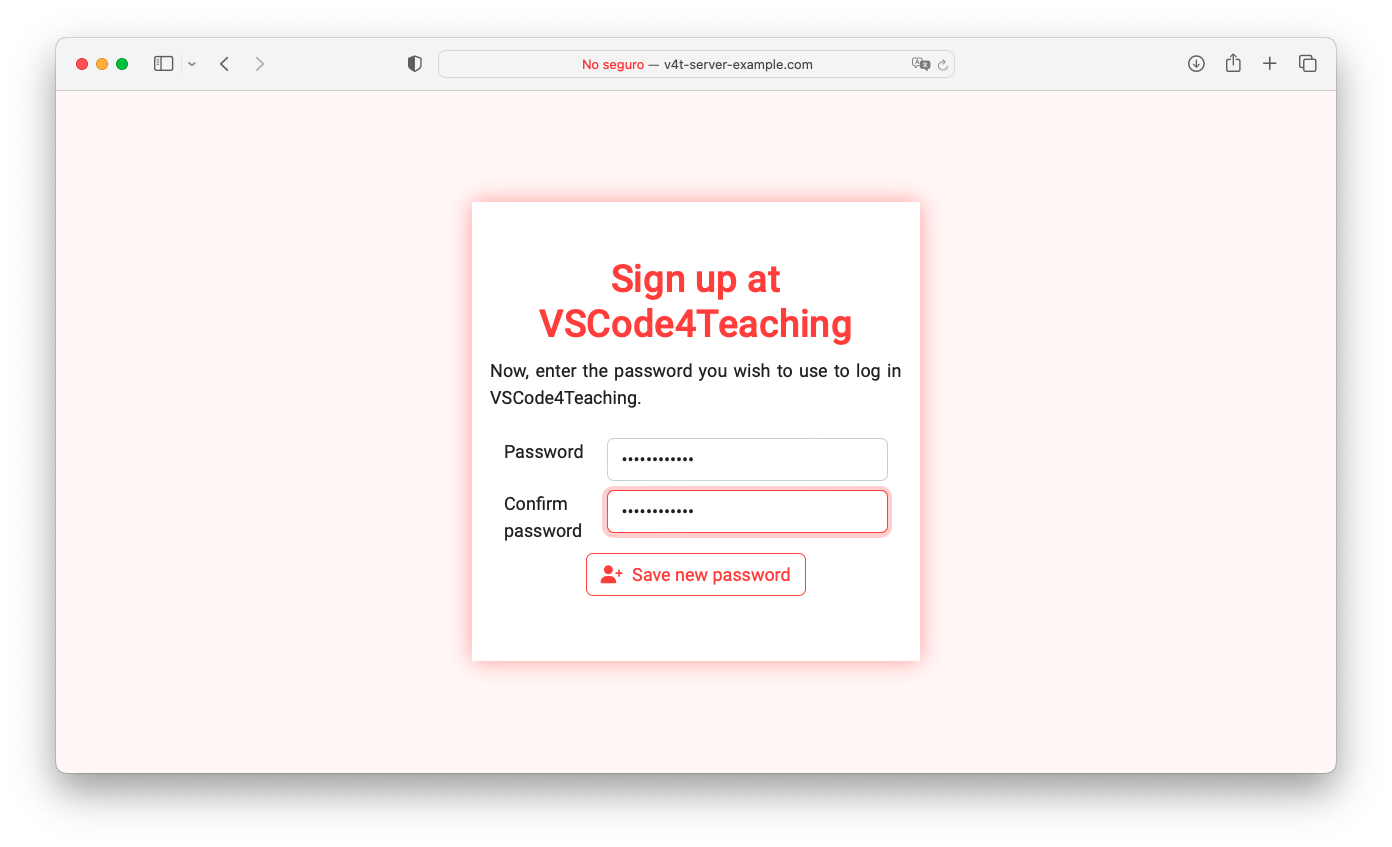
\includegraphics[width=\textwidth]{imagenes/utilizadas/4-3-implementacion/rf1-1.png}
    \caption{Captura del navegador web durante el proceso de configuración de contraseña de un nuevo profesor.}
    \label{fig:reqf1-1}
\end{figure}

\subsubsection{\texttt{RF-2}: alta simultánea de ejercicios}
\label{subsec:rf2}

Uno de los procesos más habitualmente repetidos en \textit{VSCode4Teaching} es, desde su primera versión, la subida o adición de nuevos ejercicios dentro de los cursos por parte de los profesores. Este proceso requería necesariamente rellenar un campo de texto con el nombre del ejercicio y seleccionar el fichero, directorio o conjunto de ambos que conformaba la plantilla, subiéndola al servidor y proporcionándosela al alumnado cuando descargasen el ejercicio por primera vez para tomarla como base de su propia propuesta de resolución.

La implementación de este requisito busca crear una nueva forma de subir los ejercicios que simplifique el proceso anteriormente descrito y permita, además, añadir varios ejercicios de una sola vez. En la \referenciaFigura{fig:reqf2-1} se muestra una captura de la extensión en la que se señala el botón para añadir un solo ejercicio (en verde) y el nuevo botón que da acceso a la funcionalidad para subir varios ejercicios en una sola acción (en naranja).

Gracias a la incorporación de esta nueva funcionalidad, los profesores pueden subir varios ejercicios de forma simultánea seleccionando un directorio que tenga en su interior una carpeta para cada ejercicio que se desea crear, de forma que se toma el nombre de cada directorio como el del nuevo ejercicio ---siendo modificable posteriormente---; y sus contenidos, como la plantilla del ejercicio (y la solución, en caso de incluirla, tal como se refleja en la \referenciaSeccion{subsec:rf5}).

\begin{figure}[ht]
    \centering
    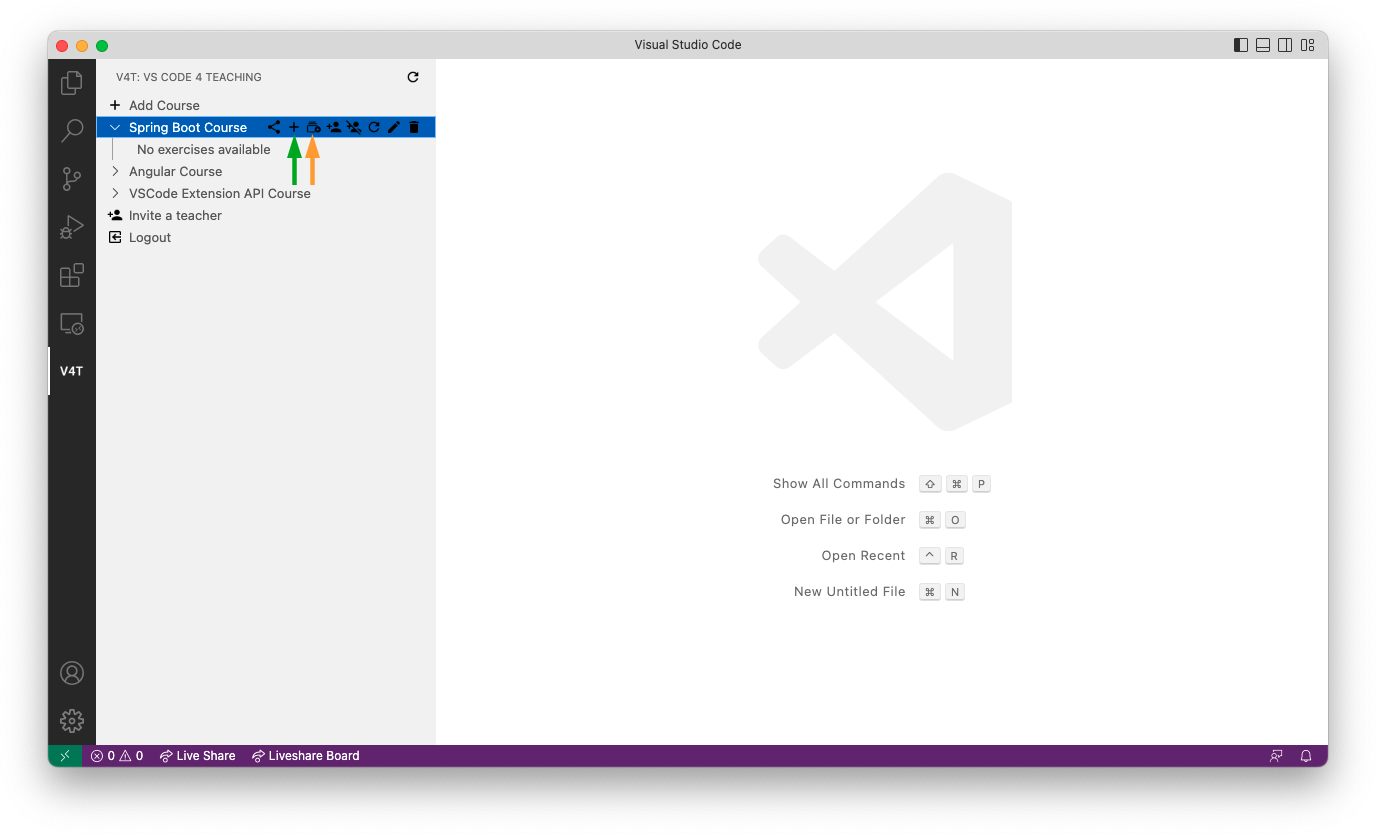
\includegraphics[width=0.975\textwidth]{imagenes/utilizadas/4-3-implementacion/rf2-1.png}
    \caption{Captura de la extensión en la que se destacan los botones empleados para añadir ejercicios.}
    \label{fig:reqf2-1}
\end{figure}

\subsubsection{\texttt{RF-3}: anonimato de propuestas de estudiantes}
\label{subsec:rf3}

Cuando un profesor descargaba un ejercicio en las primeras versiones de \textit{VSCode4Teaching}, la estructura de ficheros que se habilitaba en su entorno de desarrollo incluía un directorio ``template'' con la plantilla original del ejercicio y tantos directorios como propuestas de alumnos terminadas o parcialmente guardadas hubiese, identificando cada una de ellas con el nombre de usuario del alumno. Además, el \textit{dashboard} ---creado para que los profesores pudieran obtener información del progreso de sus estudiantes en la realización de los ejercicios--- incluía como elemento principal una tabla que reflejaba nombre, apellidos, nombre de usuario y fecha de última modificación para cada uno de los estudiantes del curso.

En cumplimiento del primer objetivo de los recogidos en el \referenciaCapitulo{cap:objetivos}, la presente tarea conduce a la modificación de los mecanismos de identificación de las propuestas de resolución de los ejercicios remitidas por los estudiantes con el fin de poder garantizar su anonimato. Para ello, se introducen dos requisitos derivados:

\begin{itemize}
    \item El requisito \texttt{RF-3.1} establece la necesidad de alterar el sistema de nomenclatura que se emplea para almacenar las propuestas enviadas por los estudiantes. Como consecuencia, se introduce una modificación por la que el servidor asigna como nombre del directorio de cada una de ellas un texto del formato ``student\_\texttt X'', siendo \texttt X el número identificador de la propuesta almacenado en base de datos. Este formato permite cotejar el número empleado para formar el nombre del directorio (\texttt X) con los datos persistidos, pudiendo así relacionar la propuesta de cada estudiante con su propia información de forma rápida. La \referenciaFigura{fig:reqf3-1} recoge una comparativa entre los formatos anterior y actual.
    \item El requisito \texttt{RF-3.2} estipula las dos actuaciones que se ejecutan sobre el \textit{dashboard}: la modificación de la columna que recoge el nombre de usuario de los estudiantes, introduciendo en ella el nombre del directorio que recoge su propuesta de solución; y la introducción de un elemento de control interactivo que permita a los docentes ocultar o mostrar la columna de nombres y apellidos a elección. En la \referenciaFigura{fig:reqf3-2} se destaca este elemento de control y se puede visualizar la tabla sin y con la mencionada columna cuando este está activado y desactivado, respectivamente.
\end{itemize}

De este modo, la ejecución de ambos requisitos permite lograr una situación de total anonimato de los estudiantes si así lo desea el docente, pudiendo relacionar cada nombre de directorio con el nombre propio y los apellidos de cada estudiante en el \textit{dashboard} cuando lo desee.

\begin{figure}[ht]
    \centering
    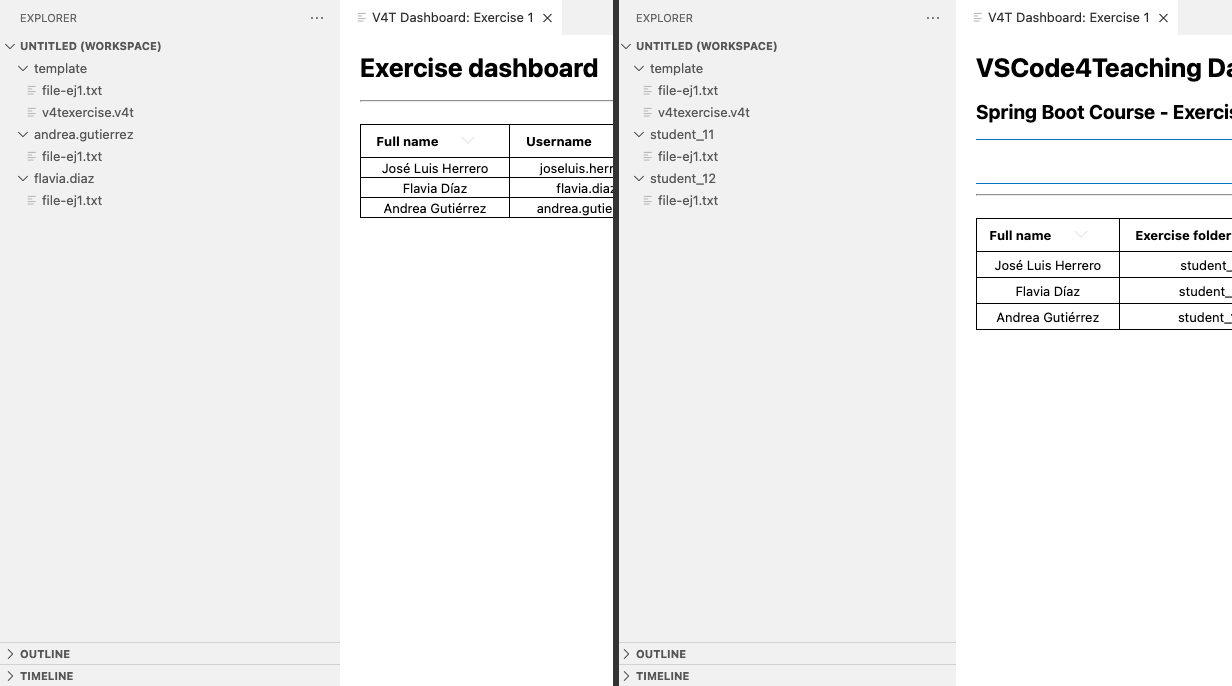
\includegraphics[width=\textwidth]{imagenes/utilizadas/4-3-implementacion/rf3-1.png}
    \caption{Comparativa entre los formatos anterior (izquierda) y actual (derecha) de almacenamiento de propuestas de estudiantes.}
    \label{fig:reqf3-1}
\end{figure}

\begin{figure}[ht]
    \centering
    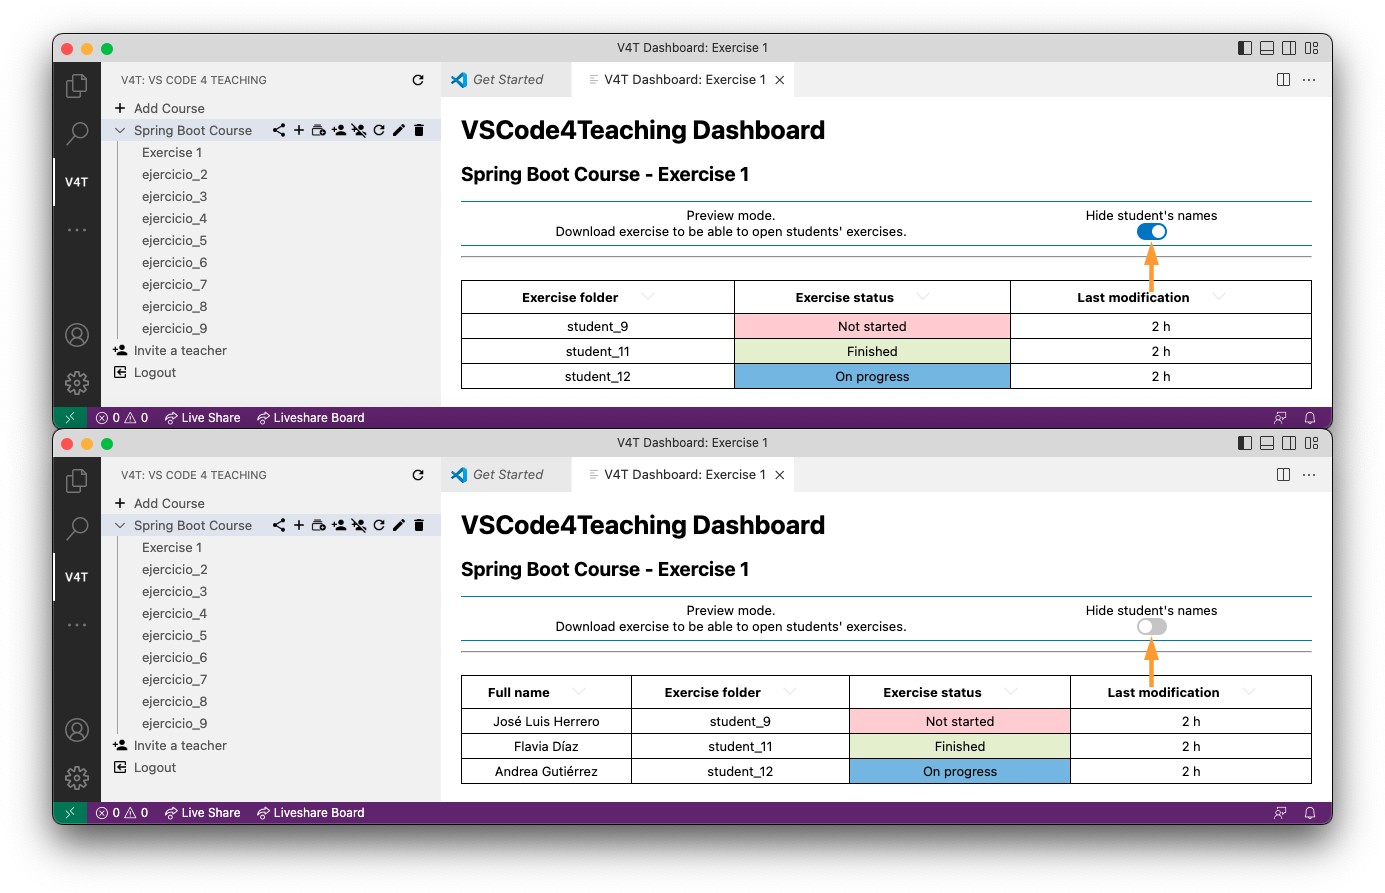
\includegraphics[width=0.975\textwidth]{imagenes/utilizadas/4-3-implementacion/rf3-2.png}
    \caption{Captura de la extensión en la que se destaca el nuevo elemento para ocultar y mostrar la identidad de los estudiantes.}
    \label{fig:reqf3-2}
\end{figure}

\subsubsection{\texttt{RF-4}: previsualización del \textit{dashboard}}
\label{subsec:rf4}

La versión de \textit{VSCode4Teaching} tomada como punto de partida para el inicio del presente TFG incluía ya un \textit{dashboard} completamente funcional que requería que el profesor tuviese descargado el ejercicio completo en su propio espacio de trabajo en Visual Studio Code para poder ejecutar las funcionalidades de apertura de ficheros y visualización de diferencias con la plantilla, que se ejecutan mediante botones situados en cada fila de la tabla mostrada en esta visualización.

El presente requisito busca eliminar la necesidad de descargar todos los ficheros de los ejercicios y permitir a los profesores visualizar el \textit{dashboard} ---sin acceso a las funcionalidades anteriormente nombradas--- para el ejercicio que deseen con independencia del que tengan activo en su espacio de trabajo. Este formato de ``previsualización'' conlleva modificaciones del \textit{dashboard}, que únicamente deberá mostrar la columna con las acciones anteriormente citadas si se abre en ``modo completo'' ---es decir, tal como se venía haciendo en versiones anteriores---. Los profesores pueden acceder a la previsualización del \textit{dashboard} de cada ejercicio haciendo uso de un nuevo botón colocado en la barra lateral junto a cada ejercicio, tal como se puede evidenciar en la \referenciaFigura{fig:reqf4-1}. Esta previsualización introduce, además, un elemento gráfico explicativo que aclara al profesor que, en caso de querer ejecutar las acciones de apertura y visualización de diferencias entre archivos, deberá descargar el ejercicio y hacer uso del \textit{dashboard} completo.

\begin{figure}[ht]
    \centering
    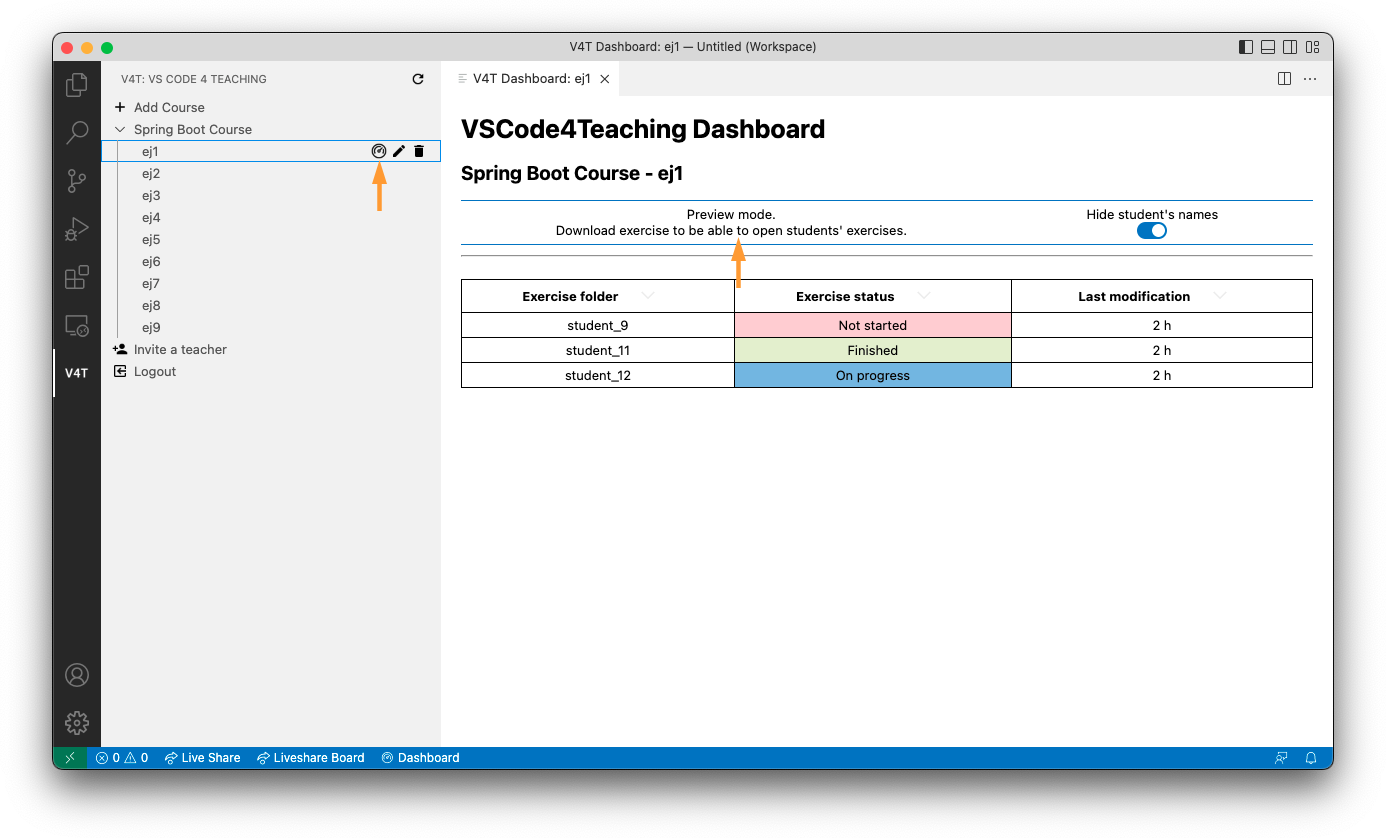
\includegraphics[width=\textwidth]{imagenes/utilizadas/4-3-implementacion/rf4-1.png}
    \caption{Captura de la extensión en la que se muestran los elementos de la GUI que permiten distinguir el modo de previsualización del \textit{dashboard}.}
    \label{fig:reqf4-1}
\end{figure}

\subsubsection{\texttt{RF-5}: guardado de soluciones de ejercicios}
\label{subsec:rf5}

Uno de los objetivos principales fijados para la evolución del proyecto \textit{VSCode4Teaching} es, tal como queda reflejado en el tercer punto del \referenciaCapitulo{cap:objetivos}, permitir al profesorado adjuntar a los ejercicios su propia propuesta de resolución, que sería accesible a los estudiantes una vez fuese publicada. Este requisito, junto con los requerimientos \texttt{RF-6}, \texttt{RF-7} y \texttt{RF-8} ---desarrollados en sendos apartados posteriores---, da cumplimiento al citado objetivo.

Con anterioridad a la implementación de este requisito, la aplicación permitía a los docentes añadir nuevos ejercicios ---tanto de uno en uno como de forma múltiple---, adjuntando a cada uno su correspondiente plantilla. Una vez implementado, se requiere a los usuarios que proporcionen un directorio por cada ejercicio y, si desean introducir solución asociada, que este contenga únicamente dos carpetas en su interior: ``template'', que recoja todos los contenidos relativos a la plantilla del ejercicio; y ``solution'', que albergue la totalidad de la propuesta de solución que se ha de adjuntar al nuevo ejercicio. Todas las estructuras distintas a la anteriormente descrita se interpretarán como plantillas incluidas para ejercicios sin solución adjunta.

La implementación de la posibilidad de incluir una solución ha tomado como base la capacidad anteriormente existente para albergar plantillas, conllevando las siguientes alteraciones:
\begin{itemize}
    \item Se ha modificado el modelo de dominio asociado a los ejercicios en el servidor para introducir la persistencia en base de datos de la información relativa a la solución siguiendo el modelo empleado para las plantillas. Asimismo, se han modificado los modelos de dominio asociados a los ejercicios en el servidor y en el cliente para introducir un valor \textit{booleano}\footnote{Booleano. También conocido como binario, es un tipo de dato que permite albergar únicamente dos posibles valores: verdadero o falso.} que almacena si un ejercicio tiene o no solución (independientemente de su disponibilidad).
    \item Se ha aprovechado el código existente para la subida de plantillas y de propuestas de estudiantes al servidor para, unificando procedimientos y eliminando bloques de código repetidos, añadir un nuevo \textit{endpoint} a la API REST para la subida de las soluciones.
    \item Se ha implementado un algoritmo en la extensión que, dado un directorio, se basa en la exploración de los contenidos de la ruta local proporcionada para determinar si la estructura de ficheros que contiene es la requerida para incluir solución o no en el momento de subir el ejercicio.
\end{itemize}

\subsubsection{\texttt{RF-6}: configuración de soluciones para profesores}
\label{subsec:rf6}

Uno de los objetivos principales fijados para la evolución del proyecto es permitir al profesorado adjuntar a los ejercicios su propia propuesta de resolución, que será accesible a los estudiantes una vez sea publicada. Este requisito es uno de los que busca dar cumplimiento al objetivo tercero del \referenciaCapitulo{cap:objetivos}.

El presente requerimiento tiene como fin la incorporación de controles que permitan a los profesores determinar cuándo es pública una solución y si los estudiantes pueden (o no) hacer modificaciones a sus propuestas propias de resolución de los ejercicios una vez hayan accedido a la solución propuesta por el docente.

De este modo, las soluciones permanecen ocultas por defecto a los estudiantes hasta que el profesor decida publicarlas, siendo este cambio irreversible; esto es, una vez publicada no puede ser despublicada. Por otro lado, el comportamiento por defecto de la aplicación es el de bloquear la edición de los ejercicios una vez el estudiante descargue la propuesta de solución del docente, pasándolo a estado ``finalizado'' automáticamente cuando el estudiante inicie la descarga de la solución, previa solicitud de confirmación. Si el docente lo desea, puede modificar este comportamiento, de modo que el estado permanecerá con el valor ``en progreso'' a pesar de haber descargado la solución, considerando que este ajuste debe estar adecuadamente configurado antes de la publicación de la solución, ya que este parámetro también permanecerá inmutable tras publicarla. Ambas modificaciones de configuración se pueden realizar a través del \textit{dashboard} de los ejercicios que tienen solución, tal como se puede apreciar en la \referenciaFigura{fig:reqf6-1}.

Para efectuar esta implementación, se han realizado los siguientes cambios:
\begin{itemize}
    \item Se han alterado los modelos de dominio de la entidad relativa a los ejercicios tanto en el servidor como en el cliente para introducir dos valores \textit{booleanos} para controlar la disponibilidad de la solución y la capacidad de edición tras su descarga.
    \item Se han introducido dos elementos de interacción de usuario en forma de casillas de verificación para dotar al profesorado de la capacidad para modificar los atributos de configuración descritos con anterioridad. Estos elementos quedan señalados en la figura anteriormente referenciada.
\end{itemize}

\begin{figure}[ht]
    \centering
    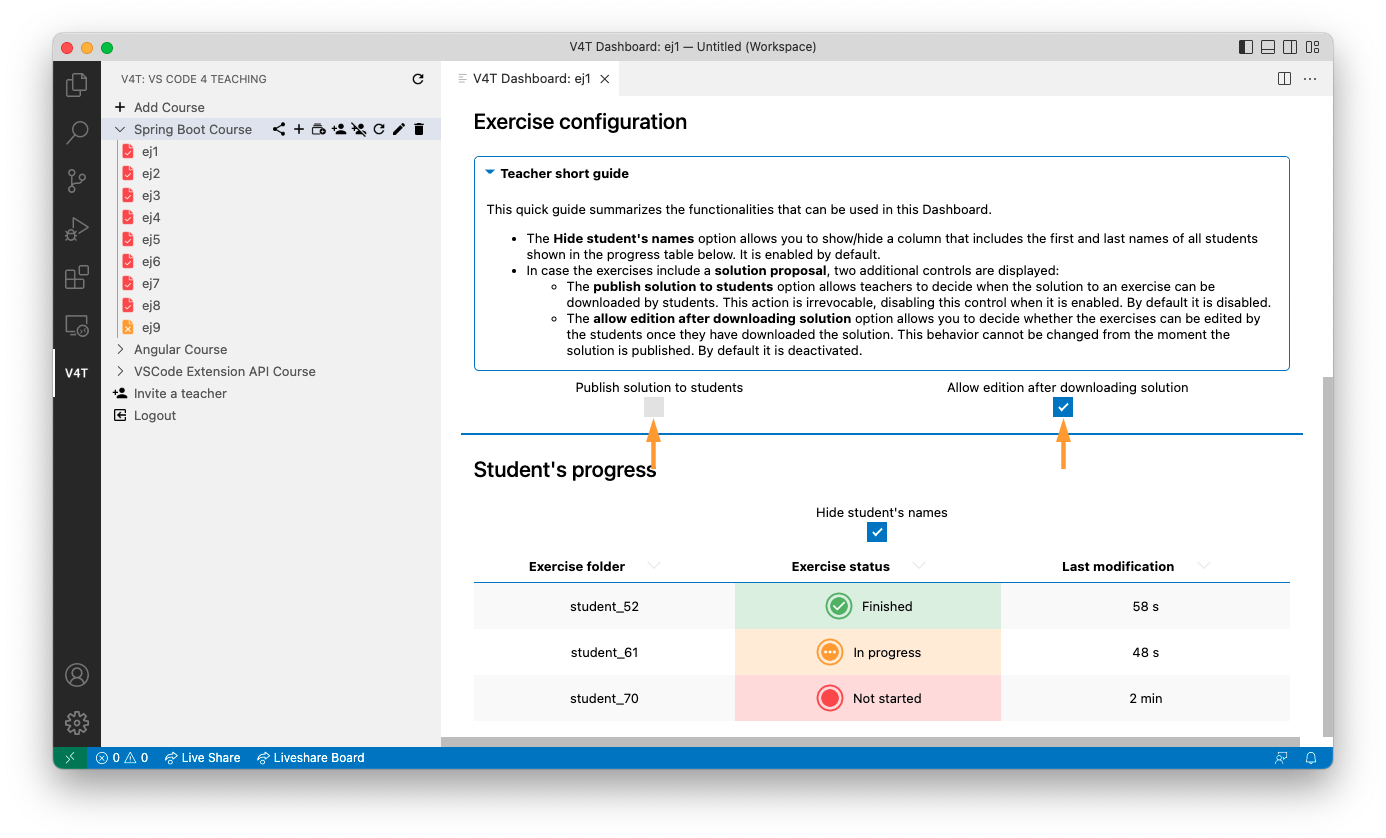
\includegraphics[width=\textwidth]{imagenes/utilizadas/4-3-implementacion/rf6-1.png}
    \caption{Captura de la extensión en la que se destacan los elementos gráficos para la modificación de la configuración de la solución de un ejercicio.}
    \label{fig:reqf6-1}
\end{figure}

\subsubsection{\texttt{RF-7}: descarga de soluciones}
\label{subsec:rf7}

Tal como se introduce en los dos epígrafes anteriores, uno de los objetivos principales fijados para la evolución del proyecto es permitir a los estudiantes descargar las propuestas de solución adjuntadas por el profesorado a los ejercicios realizados siempre y cuando hayan sido publicadas por ellos.

Este requerimiento afecta a profesores y a estudiantes de forma diferente, por lo que da lugar a en dos requisitos según el rol:
\begin{itemize}
    \item El requisito \texttt{RF-7.1} establece que los estudiantes deben poder tener acceso a la descarga de la solución de un ejercicio siempre que exista solución y que haya sido publicada por los profesores.
    
    Para incorporar este punto, se ha aprovechado la implementación del requisito \texttt{RF-7.2}, introduciendo un control específico para usuarios con rol de estudiantes sobre la disponibilidad de la solución. En caso de que se den las condiciones adecuadas, se habilita un nuevo botón para la descarga de la solución y se lanza un aviso en la parte inferior del entorno de desarrollo, tal como ilustra la \referenciaFigura{fig:reqf7-1}.

    Al presionar el botón, aparece un cuadro de diálogo modal que informa al estudiante acerca de si tendrá la capacidad de editar posteriormente su ejercicio o si se marcará automáticamente como ``finalizado'' tras descargar la solución. Una vez el estudiante confirme que desee continuar, la solución se descargará y situará en un nuevo directorio llamado ``solution'' ubicado en el nivel inmediatamente inferior al del directorio padre del ejercicio activo.

    Adicionalmente, se han ampliado las capacidades del botón de refresco de la extensión y, en caso de que haya un ejercicio activo, la acción desencadenada por su utilización también verificará si la solución ha sido publicada desde la última vez que se descargó el ejercicio, favoreciendo la usabilidad de esta funcionalidad de modo que los estudiantes no tengan que desactivar y volver a acceder un ejercicio para comprobar si la solución ya es pública.
    \item El requisito \texttt{RF-7.2} determina que los profesores deben tener acceso a la solución que han adjuntado a sus propios ejercicios ---en caso de haberla---, descargándose junto con la plantilla y las propuestas de resolución parciales o finales de los estudiantes al activar un ejercicio desde la extensión.
    
    Para ejecutar la implementación de este requisito, se han tomado como ejemplo los métodos y procedimientos dispuestos tanto en servidor como en cliente para la descarga de la plantilla, reutilizando el código ---y previniendo la aparición de duplicidades--- para la implementación de esta capacidad. Como consecuencia, la solución se descarga en paralelo a la plantilla para los profesores independientemente de su estado de publicación.
\end{itemize}

\begin{figure}[ht]
    \centering
    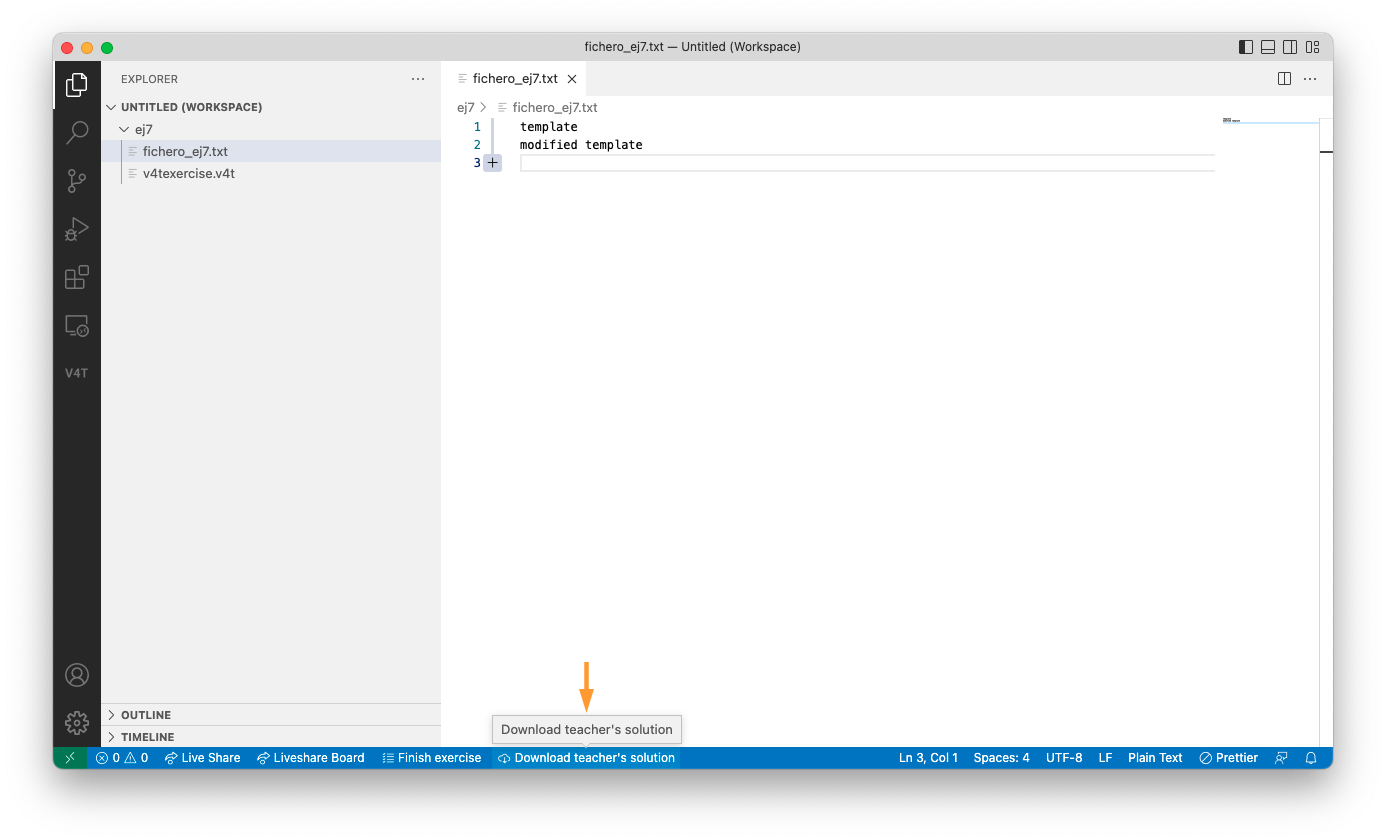
\includegraphics[width=\textwidth]{imagenes/utilizadas/4-3-implementacion/rf7-1.png}
    \caption{Captura de la extensión en la que se destaca el botón habilitado para la descarga de soluciones a ejercicios.}
    \label{fig:reqf7-1}
\end{figure}

\subsubsection{\texttt{RF-8}: visualización de diferencias con solución}
\label{subsec:rf8}

Este requisito busca completar el objetivo del \texttt{RF-7.1} ---\referenciaSeccion{subsec:rf7}---, por el que se permite a los estudiantes descargar las soluciones de los ejercicios que dispongan de ella a partir de su publicación por parte del profesor.

El presente requerimiento aborda la creación de una característica que permita a los estudiantes visualizar gráficamente las diferencias que existan entre la propuesta de solución del profesor y su propia resolución del ejercicio. Para ejecutar esta funcionalidad, se han llevado a cabo las siguientes actuaciones:
\begin{itemize}
    \item Implementación de un algoritmo basado en el recorrido recursivo en profundidad de los directorios locales para obtener estructuras de datos arborescentes en memoria que reflejasen los contenidos de los directorios asociados tanto a la propuesta del propio alumno como a la solución descargada.
    \item Diseño y confección de un algoritmo que, dadas las dos estructuras arborescentes anteriormente detalladas, genera un nuevo árbol resultante de la combinación de los nodos de ambos árboles manteniendo en memoria el árbol de origen y preservando el orden alfabético de los nodos.
    \item Incorporación de los elementos de interacción con el usuario necesarios para que los estudiantes pudiesen visualizar la relación de ficheros existentes en el árbol obtenido mediante la ejecución de los dos algoritmos anteriores junto con su procedencia, incluyendo un cuadro de diálogo que muestra los ficheros y directorios del árbol resultante de la combinación y un botón habilitado tras descargar la solución que permite ejecutar la presente funcionalidad. En la \referenciaFigura{fig:reqf8-1} se capturan sendos elementos y señalan en color naranja y verde, respectivamente.
    \begin{itemize}
        \item En caso de que se seleccione un fichero únicamente existente en uno de los dos directorios, se abrirá en una nueva pestaña del entorno de desarrollo como un fichero simple.
        \item Por otro lado, en caso de que el fichero escogido exista en ambas procedencias, se mostrará un visor de diferencias entre ambos ficheros.
    \end{itemize}
\end{itemize}

\begin{figure}[ht]
    \centering
    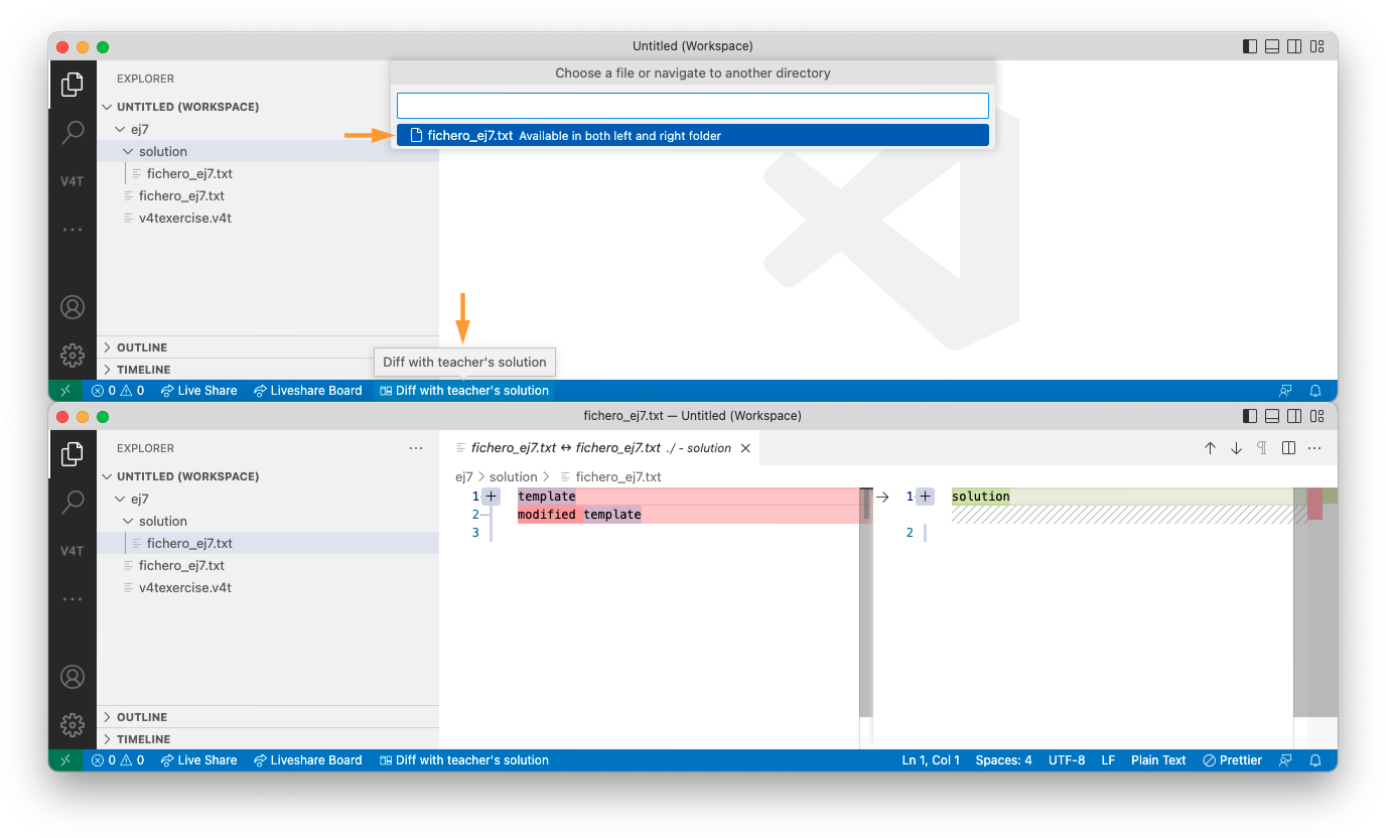
\includegraphics[width=\textwidth]{imagenes/utilizadas/4-3-implementacion/rf8-1.png}
    \caption{Captura de la extensión en la que se ejecuta la diferenciación entre la solución del docente y la propuesta del estudiante.}
    \label{fig:reqf8-1}
\end{figure}

\subsubsection{\texttt{RF-9}: página de ayuda personalizada}
\label{subsec:rf9}

Uno de los objetivos de la presente evolución de \textit{VSCode4Teaching} es el de favorecer una mejor interacción entre los usuarios y la aplicación, haciéndola más intuitiva y fácil de usar, tal como establece el punto cuarto de los objetivos establecidos en el \referenciaCapitulo{cap:objetivos}.

En las versiones previas de \textit{VSCode4Teaching} se implementó un formato de inscripción en los cursos con el siguiente flujo de operaciones asociado: el profesor disponía de un botón para generar un código de invitación para estudiantes, quienes debían introducirlo en un cuadro de diálogo con su sesión abierta en la extensión para matricularse en el curso. Este proceso puede resultar complejo si se carece de una explicación adecuada previa.

En línea con el objetivo establecido, se ha aprovechado la introducción de la nueva aplicación web ---véase la \referenciaSeccion{sec:diseñoArquitectura} a este respecto--- para crear una página de ayuda nueva. De este modo, de ahora en adelante, el profesor genera un enlace de invitación a una página web (y no únicamente un código) que los estudiantes reciben y abren en su navegador web, donde pueden encontrar una página de ayuda como la que se refleja en la \referenciaFigura{fig:reqf9-1}. Esta página muestra una primera invitación que varía según el código introducido, reflejando el nombre del profesor y del curso al que se ha invitado al alumno, pudiendo así garantizar \textit{a priori} que se ha recibido el enlace de invitación correcto. A continuación, se introduce una serie de imágenes animadas que permiten a los estudiantes tener un primer acercamiento con el funcionamiento de \textit{VSCode4Teaching} y familiarizarse con las funcionalidades que tienen disponibles. Además, en el punto en que se explica cómo inscribirse al curso haciendo uso del código, disponen de un campo especial con un botón que les permite copiar al portapapeles este código fácilmente.

\begin{figure}[ht]
    \centering
    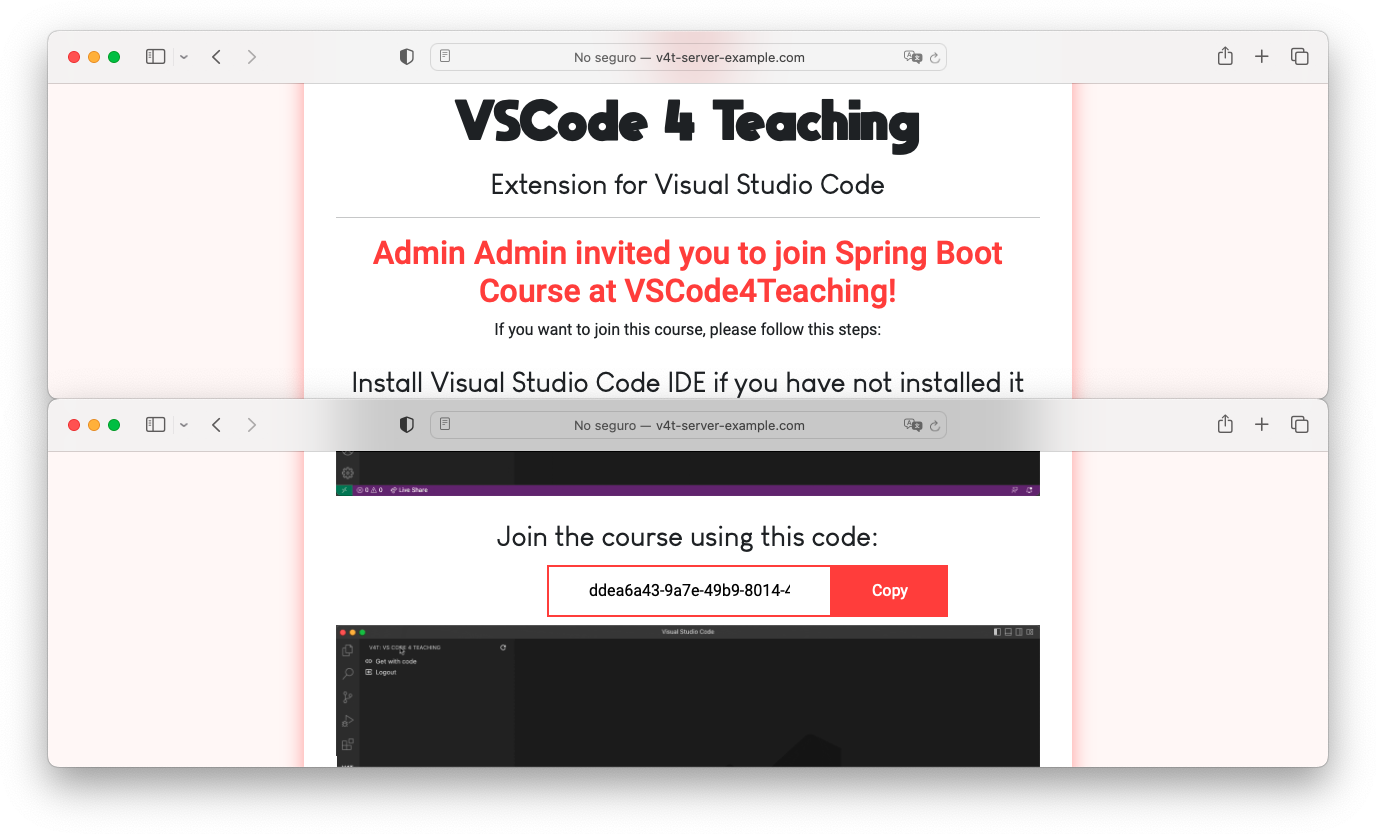
\includegraphics[width=\textwidth]{imagenes/utilizadas/4-3-implementacion/rf9-1.png}
    \caption{Captura de la página de ayuda personalizada según el código de invitación a curso suministrado.}
    \label{fig:reqf9-1}
\end{figure}

\subsubsection{\texttt{RF-10}: menú contextual en cursos}
\label{subsec:rf10}

En la extensión para Visual Studio Code, los usuarios pueden visualizar, con independencia de su rol, una lista de cursos y ejercicios. Los cursos tienen asociadas una serie de acciones ejecutables. Mientras que los estudiantes únicamente pueden refrescar el curso para actualizar sus ejercicios asociados, los docentes tienen disponibles las opciones para: compartir el enlace de invitación al curso, añadir nuevos ejercicios de forma simple o múltiple, inscribir o eliminar usuarios manualmente, refrescar la lista de ejercicios, modificar el nombre del curso o eliminarlo.

Todas estas acciones están asociadas a iconos. La ingente cantidad de iconos mostrados a los usuarios puede hacer que, hasta que no estén totalmente familiarizados con el uso de la aplicación, necesiten comprobar cuál es la finalidad de cada uno de ellos antes de accionarlos. Como consecuencia, en aras de una mejor interacción y con el fin de cumplir el segundo objetivo del TFG ---acerca de una mejor interacción usuario-aplicación, véase el \referenciaCapitulo{cap:objetivos}---, se ha implementado la posibilidad de visualizar un menú contextual que explica las acciones ejecutables mediante texto en lugar de iconos, haciéndolo más fácilmente comprensible, tal como se puede visualizar en la \referenciaFigura{fig:reqf10-1}. Para poder abrir este menú, los usuarios únicamente deben hacer \textit{click} secundario ---gesto habitualmente empleado para la apertura de este tipo de menús--- sobre un curso en la vista lateral de la extensión.

\begin{figure}[ht]
    \centering
    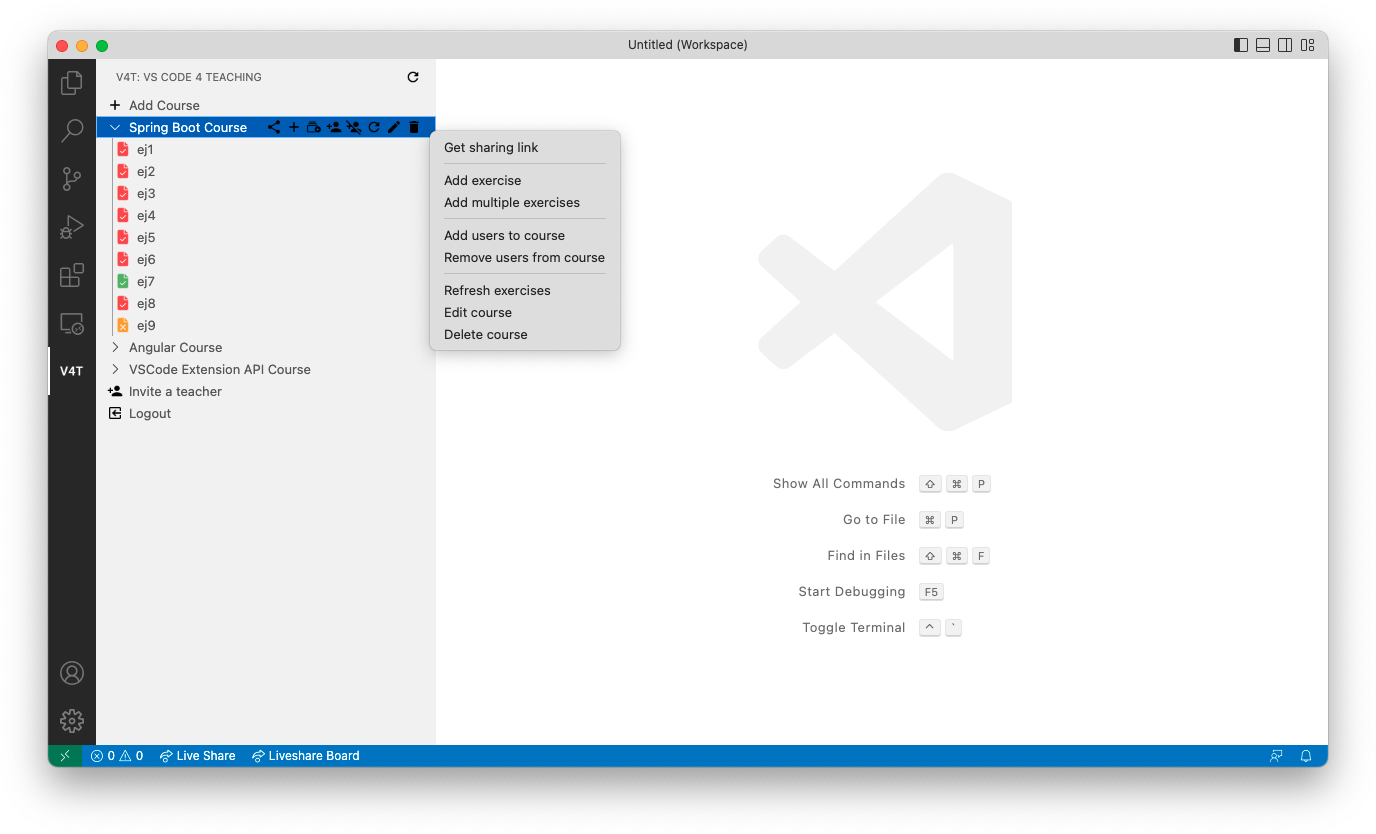
\includegraphics[width=\textwidth]{imagenes/utilizadas/4-3-implementacion/rf10-1.png}
    \caption{Menú mostrado a los docentes al hacer \textit{click} secundario sobre un curso.}
    \label{fig:reqf10-1}
\end{figure}

\subsubsection{\texttt{RF-11}: iconos de color para ejercicios}
\label{subsec:rf11}

Las aplicaciones que cuentan con GUI, como es el caso de \textit{VSCode4Teaching}, requieren que la interacción entre el usuario y los componentes que emplean sea lo más intuitiva y sencilla posible, buscando mostrar la información solicitada de forma clara y ágilmente interpretable, disponiendo los elementos necesarios para que el usuario actúe en consecuencia intercambiando nueva información con la aplicación, conduciendo a un uso fluido que satisfaga sus necesidades. Este hecho viene apoyado por el objetivo cuarto del Trabajo Fin de Grado ---véase el \referenciaCapitulo{cap:objetivos}---, que especifica que se deben incorporar mejoras visuales en la interfaz de usuario para facilitar el uso de la aplicación.

Gracias a la implementación del presente requisito, todos los usuarios de la aplicación ---con independencia de su rol--- visualizrán un nuevo icono junto a cada uno de los ejercicios disponibles.

Como la información que busca reflejar el icono es distinta para cada uno de los roles ---y, en consonancia, el propio icono---, se establecen dos requisitos derivados:
\begin{itemize}
    \item El requisito \texttt{RF-11.1} es el destinado a los estudiantes, estableciendo que el icono debe mostrar el estado en que se encuentra el ejercicio (pudiendo ser ``no comenzado'', ``en progreso'' o ``finalizado''). En la \referenciaFigura{fig:reqf11-1} se pueden apreciar los iconos mostrados a los estudiantes (en la parte izquierda): el ejercicio ``ej8'' tiene asociado el icono verde, asociado al último estado; ``ej9'', el icono amarillo ---reflejando estado ``en progreso''---; y ``ej7'', el icono rojo, que indica que el estudiante no ha comenzado el ejercicio.
    \item Análogamente, el requisito \texttt{RF-11.2} fija que los profesores visualicen un icono que aluda a la existencia de una solución adjunta al ejercicio y, en caso de haberla, que indique su disponibilidad. La \referenciaFigura{fig:reqf11-1} (en la parte derecha) ilustra los tres iconos disponibles para mostrar junto a cada ejercicio: el icono amarillo del ejercicio ``ej9'' indica que no tiene solución asociada; el rojo del ejercicio ``ej7'', que la solución adjunta no es pública; y el verde del ejercicio ``ej8'', que la solución ha sido publicada a los estudiantes.
\end{itemize}

Asimismo, la semántica de estos iconos también se refleja en el \textit{tooltip}\footnote{\textit{Tooltip}. Es un elemento textual que aparece en la interfaz de usuario cuando este mantiene el cursor encima de un ejercicio sin presionarlo durante varios segundos.}, en el que los estudiantes pueden visualizar entre paréntesis el estado del ejercicio en formato textual; y los docentes, una descripción sobre el estado de existencia y disponibilidad de la solución.

\begin{figure}[!ht]
    \centering
    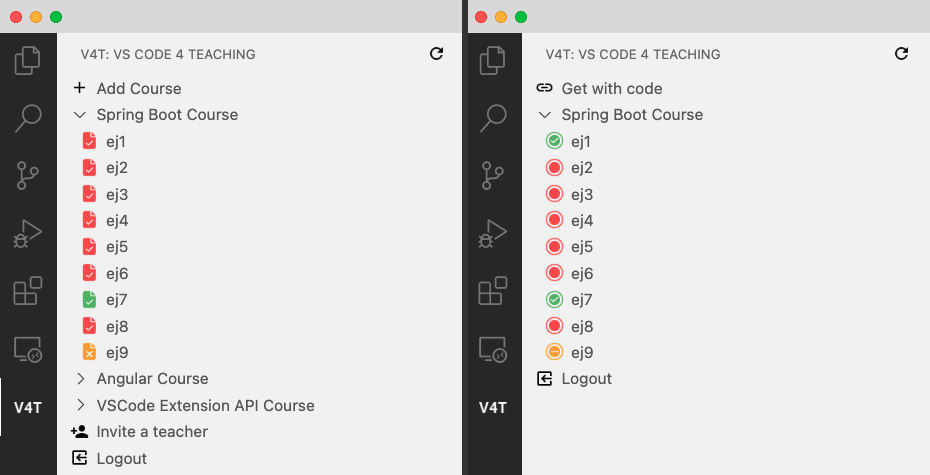
\includegraphics[width=\textwidth]{imagenes/utilizadas/4-3-implementacion/rf11-1.png}
    \caption{Iconos mostrados junto a cada ejercicio para los estudiantes (izquierda) y profesores (derecha).}
    \label{fig:reqf11-1}
\end{figure}

\subsubsection{\texttt{RF-12}: rediseño del \textit{dashboard}}
\label{subsec:rf12}

El cuarto objetivo del Trabajo Fin de Grado es lograr un mayor nivel de intuitividad en la extensión, potenciando la interacción entre usuario y aplicación mediante elementos de la GUI que permitan, entre otras finalidades, que los usuarios ---y, específicamente en este caso, los docentes--- reciban la información proporcionada por la extensión de una forma legible, visual y clara.

Las versiones previas de \textit{VSCode4Teaching} incorporaban un \textit{dashboard} que cumplía su función adecuadamente, ya que mostraba el progreso de los estudiantes en tiempo real, aportando para cada uno datos como nombre y apellidos, nombre de usuario, el tiempo transcurrido desde la última modificación y el estado del ejercicio; pero que contaba con una estética poco desarrollada y que no mostraba métricas como, por ejemplo, la cantidad de alumnos que no habían comenzado aún el ejercicio o cuántos lo habían finalizado ya. Esta versión del \textit{dashboard} puede ser visualizada en la \referenciaFigura{fig:reqf12-1}.

\begin{figure}[ht]
    \centering
    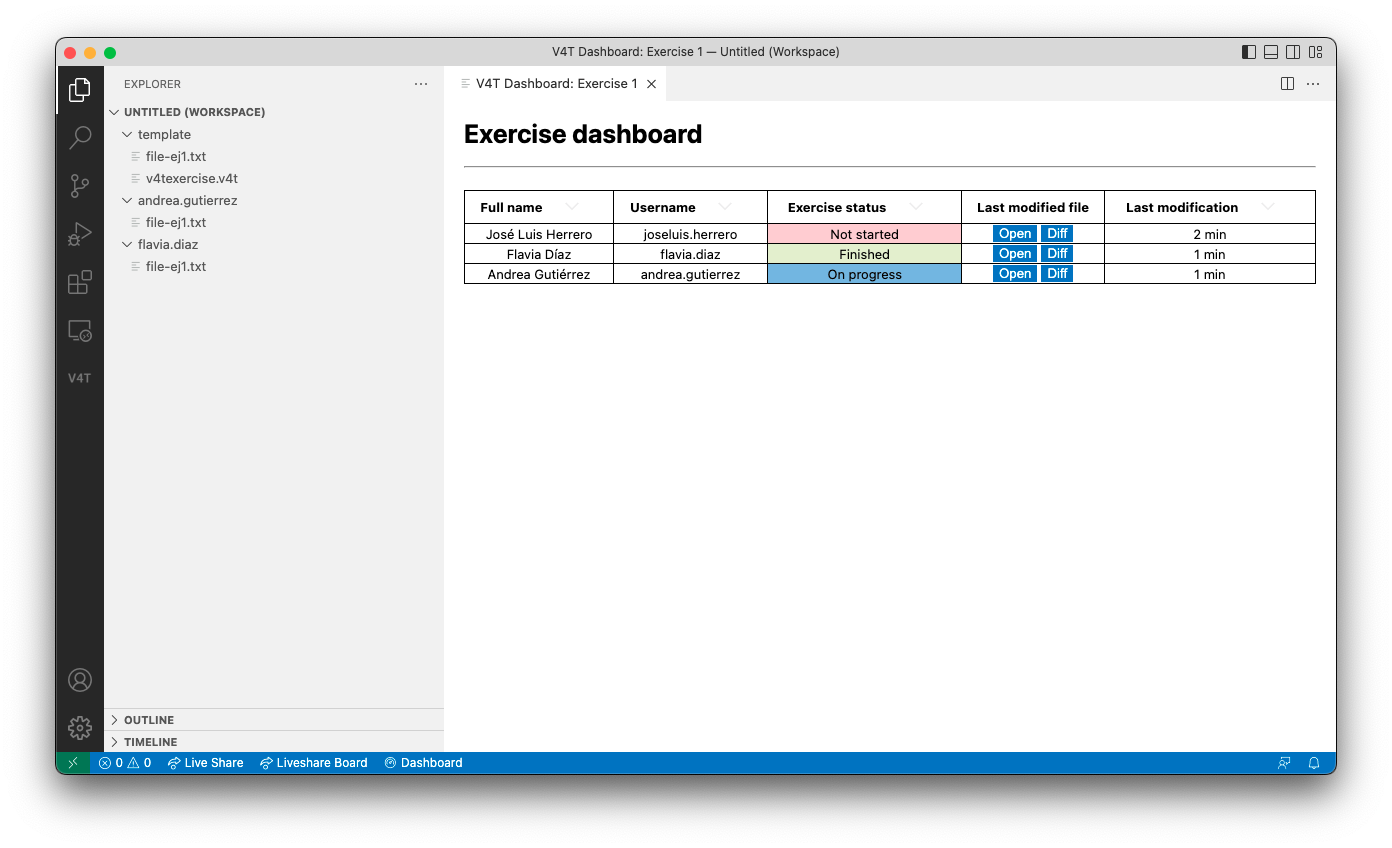
\includegraphics[width=0.925\textwidth]{imagenes/utilizadas/4-3-implementacion/rf12-1.png}
    \caption{Captura del \textit{dashboard} de \textit{VSCode4Teaching} previa a su modificación visual.}
    \label{fig:reqf12-1}
\end{figure}

\begin{figure}[ht]
    \centering
    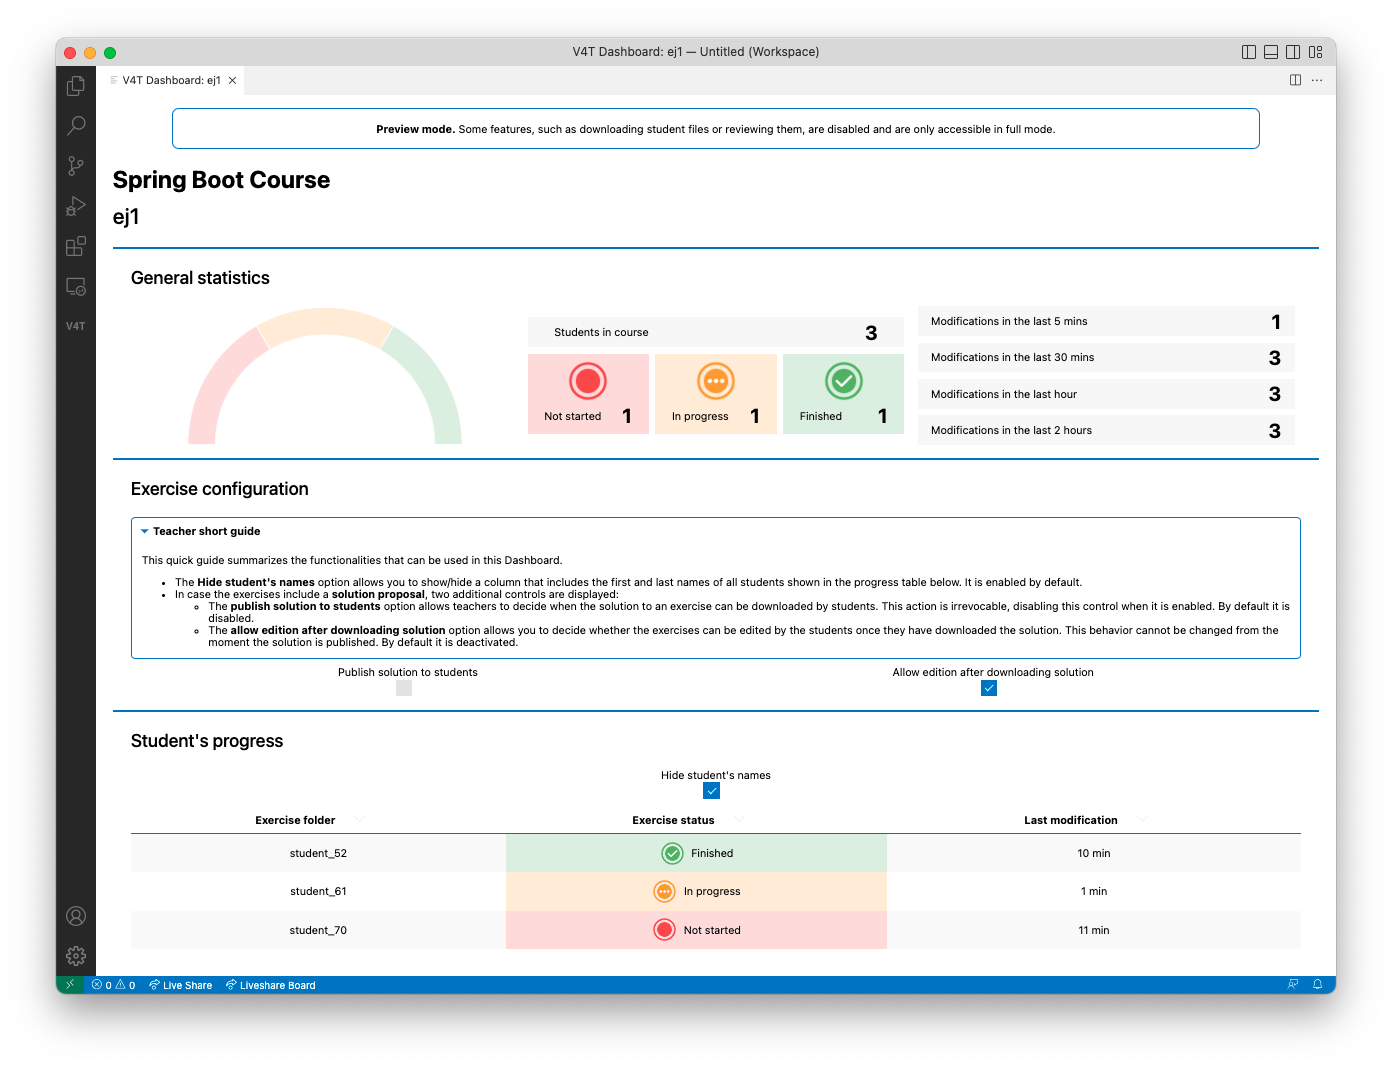
\includegraphics[width=0.925\textwidth]{imagenes/utilizadas/4-3-implementacion/rf12-2.png}
    \caption{Instantánea del \textit{dashboard} de \textit{VSCode4Teaching} tras su rediseño.}
    \label{fig:reqf12-2}
\end{figure}

Unificando el objetivo cuarto del proyecto \textit{VSCode4Teaching} ---véase \referenciaCapitulo{cap:objetivos}--- con la necesidad de generar una estética mejor y más funcional para el \textit{dashboard}, se ha ejecutado una labor de rediseño basada en tres ejes principales: la introducción de un gráfico semicircular que muestra la evolución del conjunto de estudiantes en la realización del ejercicio y la proporción de estudiantes que hay en cada uno de sus posibles estados, la introducción de nuevos parámetros estadísticos basados en el recuento de estudiantes presentes en cada uno de los estados del ejercicio y en la consideración del tiempo transcurrido en bloques de 5, 30, 60 y 120 minutos y la introducción de una guía de ayuda a docentes para explicar rápida y concisamente la funcionalidad de cada uno de los elementos de control y configuración presentes en el \textit{dashboard}.

Se introduce una instantánea del nuevo \textit{dashboard} en la \referenciaFigura{fig:reqf12-1} que, por comparación con la \referenciaFigura{fig:reqf12-2}, permite evidenciar la evolución introducida y la labor de rediseño ejecutada en una nueva visualización que cuenta con tres secciones claramente diferenciadas: una de estadísticas generales, en la que se introducen los nuevos elementos gráficos citados con anterioridad, otra de configuración en la que los docentes pueden acceder a la guía rápida y a la configuración sobre la solución ---en caso de haberla--- y una sección de progreso individual de los estudiantes, que muestra una tabla de estética mejorada con la información y funcionalidad que venía estando disponible en versiones anteriores.


\subsection{Requisitos no funcionales}
\label{subsec:reqsNoFuncionales}
\subsubsection{\texttt{RN-1}: ciberseguridad y mantenimiento preventivo}
\label{subsec:rn1}

La ciberseguridad es la ``práctica de proteger sistemas, redes y programas de ataques digitales [...] que apuntan a acceder, modificar o destruir la información confidencial, extorsionar a los usuarios o interrumpir la continuidad del negocio'' \cite{rn1_queEsCiber}.

De esta definición se extrapola el papel fundamental que la seguridad informática ocupa en el desarrollo y mantenimiento de todos los programas, generando un trabajo constante y necesario de detección y solución de problemas en materia de confidencialidad, integridad y disponibilidad ---los pilares básicos de la seguridad informática--- de las herramientas informáticas y los datos que involucran en su uso.

Durante el desarrollo de este Trabajo Fin de Grado, han sido detectadas numerosas vulnerabilidades en las dependencias y \textit{frameworks} empleados para la implementación de \textit{VSCode4Teaching}, condición suficiente para la introducción de cuatro \textit{sprints} o pequeños periodos de tiempo dedicados específicamente a la actualización de estas librerías a sus últimas versiones disponibles.

El servidor ha sido el más afectado por las vulnerabilidades surgidas en los últimos meses. Alrededor de este componente, que se basa en el uso del \textit{framework} Spring ---véase \referenciaSeccion{subsec:tecServidor} para más información---, han aparecido importantes vulnerabilidades. Algunas de las más destacadas han sido catalogadas en la lista \textit{Common Vulnerabilities and Exposures} (CVE\footnote{CVE. Siglas de ``vulnerabilidades y revelaciones comunes'' (del inglés \textit{Common Vulnerabilities and Exposures}). Es una de las listas de recopilación de vulnerabilidades y riesgos de seguridad más extendidas actualmente.}) \cite{rn1_cve} como: CVE-2021-44228, CVE-2021-45046, CVE-2021-45105 (noviembre-diciembre 2021, conocidas como ``Log4j'') y CVE-2022-22965 (enero 2022, conocida como ``Spring4Shell''). Como consecuencia, se ha introducido una actualización de la versión de Spring Boot a la más reciente disponible en la fecha de cierre del trabajo (2.7.5), así como de las dependencias empleadas para el funcionamiento del servidor.

Asimismo, sobre la extensión para Visual Studio Code se han ejecutado actualizaciones de dependencias y \textit{frameworks} para introducir correcciones a vulnerabilidades como las identificadas como CVE-2021-3918 (noviembre 2021), CVE-2021-44906 (diciembre 2021) o CVE-2022-0155 (enero 2022), así como actualizaciones de las diversas librerías empleadas a las últimas versiones divulgadas.

La aplicación web SPA también ha recibido diversas actualizaciones, aplicadas tanto a su \textit{framework} de base, Angular (actualizado a versión 14.2.11) como a alguna de sus dependencias por motivo de mejora en materia de seguridad y de rendimiento.

\subsubsection{\texttt{RN-2}: sistemas de registro de eventos}
\label{subsec:rn2}

La mantenibilidad es uno de los atributos de calidad esenciales en todos los proyectos \textit{software}, especialmente en aquellos con naturaleza de código libre como \textit{VSCode4Teaching}. Es por ello que resulta crucial introducir requisitos que permitan dar una evolución y mantenimiento adecuados a las aplicaciones para poder ejecutar desarrollos posteriores de forma más sencilla y rápida. Una de estas herramientas son los sistemas de registro de eventos o \textit{logs} y que permiten a los desarrolladores depurar y comprender el funcionamiento de las aplicaciones de forma más adecuada en tiempo real mientras funcionan, dejando constancia escrita de aquellas acciones que se deseen registrar a medida que suceden durante el uso de la aplicación.

\textit{VSCode4Teaching} introduce sistemas de registro de eventos en sus tres componentes, potenciando el uso de los anteriormente existentes e incorporando nuevas librerías que permiten organizarlos de forma más adecuada. El servidor introduce la biblioteca \textit{Log4J} \cite{rn2_tecLogServidor}, que está integrada dentro del \textit{framework} Spring en el que se basa ---tal como queda reflejado en la \referenciaSeccion{subsec:tecServidor}---, potenciando su utilización mediante la revisión de los eventos inventariados anteriormente existentes y la introducción de registros de actividades como la recepción y gestión de peticiones y el envío de sus respectivas respuestas.

Por otro lado, la extensión introduce la librería \textit{Winston} \cite{rn2_tecLogExtension} con el mismo propósito, permitiendo generar una traza de las peticiones que, cotejándolo con el registro anteriormente comentado, permite analizar su interacción con el servidor, recogiendo las peticiones enviadas y recibidas, las demoras temporales que se producen o el estado del cuerpo de las peticiones en su envío y en su recepción.

Asimismo, aunque su utilización es menor, también se introduce en la aplicación web SPA la librería \textit{ngx-logger} \cite{rn2_tecLogAppWeb} y se reflejan registros de las peticiones que envía al servidor durante los procesos de usuario ejecutados en este componente.

\subsubsection{\texttt{RN-3}: generación de imagen Docker}
\label{subsec:rn3}

Tal como queda recogido en la \referenciaSeccion{sec:distribDespliegue}, el servidor de \textit{VSCode4Teaching} está preparado para ser compilado en formato de imagen Docker, permitiendo de este modo la ejecución de instancias del servidor en forma de contenedores ligeros sobre cualquier sistema operativo, añadiendo la portabilidad a la lista de atributos de calidad del proyecto.

Docker se sirve de pequeños ficheros de configuración conocidos como \textit{Dockerfile} \cite{rn3_dockerfile}, que se introducen en la raíz de los proyectos y contienen las instrucciones necesarias para, a partir del código fuente, generar la imagen divulgable e instanciable de la aplicación. En el \referenciaCodigo{cod:dockerfileAnterior} se observa la versión original del fichero \textit{Dockerfile}, que requería de la existencia previa de un artefacto JAR del servidor.

Debido a la introducción de la nueva aplicación web SPA ---véase la \referenciaSeccion{sec:diseñoArquitectura}---, que queda compilada y embebida en el servidor antes de generar su imagen, y a la necesidad de poder compilar la imagen en cualquier computador sin necesidad de que tenga instalado ninguna herramienta adicional al propio Docker, se ha rediseñado y ampliado esta configuración para que la compilación se logre a partir de la ejecución de tres pasos en cascada que quedan definidos en un fichero \textit{multi-stage}\footnote{\textit{Multi-stage}. En la generación de imágenes Docker, se dice que un fichero de configuración es \textit{multi-stage} cuando requiere de la ejecución de varias fases en contenedores distintos para crear una imagen.} \cite{rn3_multistage}, tal como queda reflejado en el \referenciaCodigo{cod:dockerfileNuevo}: compilación de la aplicación Angular, compilación del servidor con la aplicación Angular compilada embebida y generación de la imagen final apta para la ejecución del JAR obtenido.

\begin{lstlisting}[language=Dockerfile,caption={\textit{Dockerfile} original del proyecto.},label=cod:dockerfileAnterior]
FROM adoptopenjdk/openjdk11:latest
RUN apt-get update && apt-get install -y netcat && rm -rf /var/lib/apt/lists/*
COPY ./target/vscode4teaching-server-*.jar ./app/vscode4teaching-server-*.jar
COPY ./docker/waitDB.sh ./app/waitDB.sh
EXPOSE 8080
RUN ["chmod", "+x", "./app/waitDB.sh"]
CMD ["./app/waitDB.sh"]
\end{lstlisting}

\begin{lstlisting}[language=Dockerfile,caption={\textit{Dockerfile} actualizado para introducir la compilación independiente del sistema operativo y de la aplicación web.},label=cod:dockerfileNuevo]
# Step 1: Compilation of Angular frontend
# It will be embedded as a static resource into Spring Boot backend
FROM node:16.13.2 AS angular
COPY vscode4teaching-webapp /usr/src/app
WORKDIR /usr/src/app
RUN ["npm", "install"]
RUN ["npm", "run", "build"]
# Step 2: Compilation of Maven project (generation of JAR)
FROM maven:3.8.4-jdk-11 AS builder
COPY vscode4teaching-server /data
COPY --from=angular /usr/src/app/dist /data/src/main/resources/static
WORKDIR /data
RUN ["mvn", "clean", "package"]
# Step 3: Generation of Docker image using the JAR previously built
FROM adoptopenjdk/openjdk11:latest
RUN apt-get update && apt-get install -y netcat && rm -rf /var/lib/apt/lists/*
COPY --from=builder /data/target/vscode4teaching-server-*.jar ./app/vscode4teaching-server-*.jar
COPY vscode4teaching-server/docker/waitDB.sh ./app/waitDB.sh
EXPOSE 8080
RUN ["chmod", "+x", "./app/waitDB.sh"]
CMD ["./app/waitDB.sh"]
\end{lstlisting}

Se introducen, además, ficheros \texttt{.dockerignore} \cite{rn3_dockerfile}, que permiten especificar adecuadamente qué ficheros pueden ser ignorados para compilar los componentes correctamente, permitiendo una rebaja en la cantidad de almacenamiento y recursos del computador empleados durante el proceso.
\subsubsection{\texttt{RN-4}: documentación de API REST}
\label{subsec:rn4}

Con la misma vocación de mantenibilidad que el requisito \texttt{RN-2} ---detallado en la \referenciaSeccion{subsec:rn2}---, el presente requerimiento busca potenciar la documentación del proyecto \textit{VSCode4Teaching}, entendiendo que este es uno de los pilares esenciales que permite a todos los desarrolladores ---con independencia de si pertenecen al proyecto o no--- comprender de forma sencilla y ágil el funcionamiento de la aplicación y la organización y aspecto del código fuente que lo conforma.

La API REST es el ``eje vertebrador'' que da unidad a \textit{VSCode4Teaching}, tal como se evidencia en la \referenciaSeccion{sec:diseñoArquitectura}, que introduce una disquisición exhaustiva sobre la organización de la aplicación que manifiesta, entre otros rasgos significativos, que esta API es la que permite la comunicación e interacción entre el servidor y los clientes de la aplicación, siendo el canal de comunicación de información bidireccional establecido entre los citados componentes.

Con el fin de potenciar la documentación existente en el proyecto sobre esta API, se ha introducido \textit{Swagger}, que es una tecnología que permite ``simplificar el desarrollo de APIs para usuarios, equipos y corporaciones con una plataforma de código abierto'' \cite{rn4_swagger}, que toma las declaraciones de \textit{endpoints} disponibles en el código fuente del servidor para generar su documentación automáticamente en el formato estipulado en el estándar \textit{OpenAPI}, que fue creado por un ``consorcio de [...] expertos que reconoce el inmenso valor de estandarizar cómo se describen las APIs''\cite{rn4_openapi} y que es uno de los más extendidos en la actualidad. Adicionalmente, permite la visualización gráfica de la documentación generada en un entorno intuitivo a través de cualquier navegador web haciendo uso de la herramienta \textit{Swagger UI} \cite{rn4_swaggerui}, tal como puede visualizarse en la \referenciaFigura{fig:reqn4-1}. Gracias a la incorporación de esta herramienta, se introduce en el código fuente del servidor la documentación en formato JSON según el estándar \textit{OpenAPI} de la API REST implementada, viéndose actualizado concordantemente con la modificación o ampliación de la implementación de los \textit{endpoints} que integran la API de este servidor.

\begin{figure}[ht]
    \centering
    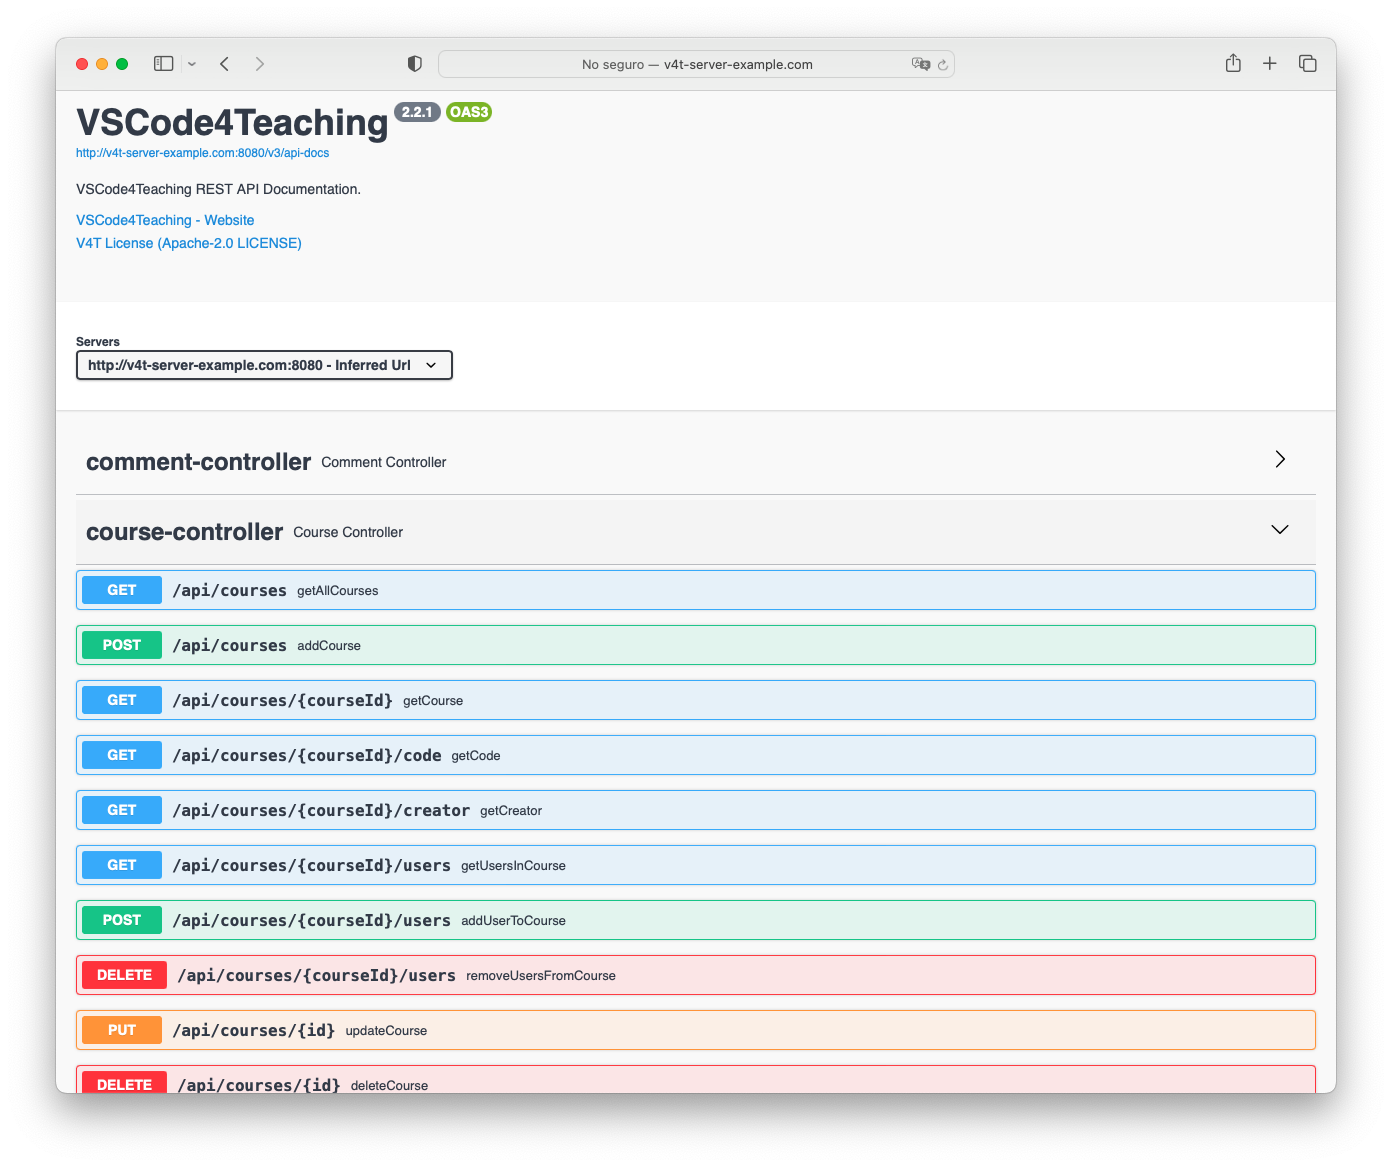
\includegraphics[width=\textwidth]{imagenes/utilizadas/4-3-implementacion/rn4-1.png}
    \caption{Vista de \textit{Swagger UI} mostrando los \textit{endpoints} disponibles en la API de VSCode4Teaching en un navegador web.}
    \label{fig:reqn4-1}
\end{figure}


\subsection{Requisitos de corrección de errores}
\label{subsec:reqsErrores}
Una vez inician su explotación ---es decir, su utilización habitual por parte de los usuarios---, las aplicaciones informáticas comienzan a registrar errores existentes en el flujo de uso, procedentes tanto de errores en la implementación de alguno de los componentes de la aplicación como de fallos en la comunicación entre ellos.

Tal como se desarrolla en la \referenciaSeccion{sec:metodologia}, la detección y corrección de errores se ha ejecutado paralelamente al desarrollo e incorporación de los demás requisitos descritos con anterioridad, ejecutando iteraciones de diagnóstico y solución de errores en tres fases: triaje del error, realizando una ``anamnesis'' para determinar las condiciones en las que se producía el error ---cuándo se producía, si se derivaba de alguna acción específica de los usuarios de un cierto rol, si sucedía periódicamente o cuáles eran las consecuencias derivadas de su ocurrencia, entre otras, con el fin de recolectar toda la información posible acerca del error---; primera implementación de una corrección, haciendo las modificaciones oportunas en el código fuente de los componentes involucrados para tratar de corregir el error; y verificación de la corrección, reproduciendo las condiciones en las que se produjo el error originalmente y evaluando si se vuelve a producir, si se produce algún otro error derivado de la corrección o si se ha subsanado en su totalidad.

El descubrimiento de nuevos errores para su posterior corrección se ha ejecutado a través de las pruebas realizadas para la verificación del \textit{software}, que se ven descritas en la \referenciaSeccion{sec:verificacion}. Las pruebas implementadas sobre el código ---esto es, las pruebas unitarias y de integración--- han permitido detectar errores lógicos mediante la comparación de resultados esperados frente a resultados obtenidos, dando lugar a algunos requisitos como el \texttt{RE-1}.
Por otro lado, las pruebas de uso en simulaciones de entornos reales han permitido encontrar fallos en la aplicación a través de la imitación de potenciales flujos de uso habituales en entornos en explotación; esto es, recreando acciones y comportamientos de usuarios, encontrando fallos que las pruebas de código implementadas para este proyecto no permiten localizar, como pueden ser los requisitos \texttt{RE-4} o \texttt{RE-6}.

Tal como se introducía en la \referenciaSeccion{subsec:listaReqsErrores}, cabe reseñar seis requisitos de entre todas las correcciones de errores ejecutados en el proyecto \textit{VSCode4Teaching}:
\begin{itemize}
    \item \texttt{\textbf{RE-1}}. Los profesores disponen de una tabla en el \textit{dashboard} para visualizar el progreso individualizado de los estudiantes en la realización de los ejercicios propuestos. Esta tabla tiene controles que permiten la ordenación de sus filas alfabéticamente según los valores de cada una de las columnas. Cuando se pretendía ordenar la tabla del \textit{dashboard} según alguna columna, el resultado de la ordenación mostrado era incorrecto, pudiendo ser ordenados por los valores de columnas diferentes o de forma aparentemente arbitraria.
    \item \texttt{\textbf{RE-2}}. Los profesores tienen a su disposición una funcionalidad para añadir varios ejercicios simultáneamente en un determinado curso. Cuando la empleaban, aparecía un directorio intermedio no existente en origen con el mismo nombre en el que se introducían todos los contenidos del ejercicio, que se mostraban en un nivel superior cuando se agregaban de uno en uno, de modo que el comportamiento de la funcionalidad daba resultados diferentes según si se ejecutaba para ejercicios individuales o para grupos de ejercicios.
    \item \texttt{\textbf{RE-3}}. Los estudiantes pueden tener los ejercicios de los cursos en los que participan en distintos estados: ``no comenzado'', cuando aún no han abierto los ejercicios en su editor de código; ``en progreso'', cuando han accedido al ejercicio en su editor; y ``finalizado'', cuando, una vez han realizado modificaciones, deciden marcarlo como finalizado, bloqueando sucesivas ediciones de su propuesta de resolución del ejercicio. Las pruebas de simulación de entornos reales permitieron detectar algunos errores que impedían que la extensión siguiese adecuadamente el progreso de los estudiantes al no modificar el estado a ``en progreso'' al comenzar el ejercicio, de modo que las modificaciones realizadas no quedaban almacenadas en el servidor. Además, una vez que los estudiantes marcaban como finalizados los ejercicios, en caso de que los descargasen de nuevo, veían revertido su estado a ``en progreso'', permitiéndoles volver a editar sus propuestas de resolución una vez marcadas como finalizadas.
    \item \texttt{\textbf{RE-4}}. En la tabla que se muestra a los profesores en el \textit{dashboard}, uno de los datos que quedan reflejados es la fecha de última modificación realizada por cada uno de los estudiantes. Este dato refleja cuánto tiempo ha transcurrido desde la última modificación registrada en base de datos, actualizándose periódicamente para reflejar valores correctos mientras se mantenga abierta esta visualización. En una prueba de simulación de entorno real se descubrió que una modificación en la interfaz de usuario de esta visualización provocó que la rutina periódica tuviese una configuración inadecuada, readaptándose para su correcta visualización en posteriores ediciones.
    \item \texttt{\textbf{RE-5}}. Cuando se producen cierres de sesión en la extensión de \textit{VSCode4Teaching}, es preciso ocultar y deshabilitar todas las funciones propias de los usuarios autenticados, ya que su utilización posterior al fin de la autenticación puede entrañar un riesgo de seguridad, pues los elementos de la interfaz de usuario que permiten la ejecución de funcionalidades como, por ejemplo, la visualización del \textit{dashboard}, de acceso restringido a profesores, quedaban visibles y funcionales en la GUI. Para eliminar este error, se introducen nuevos controles que dotan a la extensión de capacidades para eliminar todos los elementos de la interfaz que solo pueden ser ejecutados por usuarios identificados en la extensión.
    \item \texttt{\textbf{RE-6}}. Las pruebas realizadas en simulación de entornos reales permiten también detectar problemas de rendimiento y carga de la aplicación, tal como se desarrolla en la \referenciaSeccion{subsec:pruebasManuales}. Uno de los errores producidos como consecuencia de un problema de estas características se manifiesta ante la ejecución de la funcionalidad de la que los profesores disponen para cargar ejercicios de forma masiva en sus cursos. Anteriormente, se enviaban todas las peticiones para la subida de plantillas y propuestas de solución (en caso de haberlas) de forma simultánea desde la petición, ocasionando que el servidor recibiese una alta cantidad de peticiones a la vez, hecho que provocaba el incorrecto procesamiento de los ejercicios. Se ha introducido una modificación para hacer que la extensión envíe las peticiones de forma secuencial, lanzando una nueva petición cada vez que se recibe confirmación del servidor a la inmediatamente anterior, mitigando el problema de carga del servidor.
\end{itemize}



% Sección 4.4: Pruebas
%  En esta sección se describen las pruebas automáticas que han sido implementadas para el proyecto. Sobre los tests,
%  conviene indicar la cobertura del código. Si no se han implementado pruebas automáticas, deberían haberse
%  implementado y describirse aquí o tener una buena justificación de por qué no se han implementado.
\section{Verificación de \textit{software} y funcionalidad}
\label{sec:verificacion}

La verificación es un paso esencial en el desarrollo de cualquier producto \textit{software}, ya que permite determinar la adecuación de las características diseñadas e implementadas en código a los requerimientos originalmente determinados para ellas y, además, discernir cuáles son los puntos en los que la especificación original difiere con el producto obtenido con el fin de poder subsanar las diferencias.

La importancia que tiene la verificación del \textit{software} ha auspiciado la aparición de un sinfín de metodologías, técnicas y formatos para ejecutar pruebas sobre el \textit{software}. Si bien no se aplican metodologías específicas de \textit{testing} durante esta evolución, cabe reseñar que se implementan y emplean activamente múltiples tipos de pruebas, tanto automáticas como manuales.

\subsection{Pruebas automáticas}
\label{subsec:pruebasAutomaticas}
En el contexto del presente proyecto, las pruebas automáticas son todas las pruebas implementadas en código que pueden ser ejecutadas a través del sistema de integración continua ante modificaciones del código volcadas en el sistema de control de versiones. El sistema de integración continua empleado ---véase \referenciaSeccion{subsec:cicd}--- está configurado adecuadamente para ejecutar la batería completa de las pruebas automáticas introducidas en los componentes servidor y extensión del proyecto. 

Las pruebas codificadas hacen uso de dependencias o librerías específicamente creadas con el fin de verificar que los resultados obtenidos al ejecutar una determinada pieza de código coinciden con los resultados esperados. Estas pruebas basan su funcionamiento en aserciones, que determinan cuál es el resultado esperado y lo comparan con el resultado obtenido; y en dobles, que son objetos utilizados en sustitución de las dependencias empleadas para agilizar las pruebas, simulando con exactitud el comportamiento que estas dependencias tendrían en un escenario real.

Según su alcance, se distinguen dos tipos fundamentales de pruebas automáticas implementadas en el presente proyecto: las pruebas \textbf{unitarias}, que buscan verificar el funcionamiento de bloques de código ---una función, una clase o un módulo--- de forma rápida y sencilla; y las pruebas de \textbf{integración}, que son aquellas que verifican cómo se produce la interacción entre funciones, clases o módulos dentro de un mismo componente.

Se introduce a continuación un análisis de las pruebas realizadas en el servidor y en la extensión de \textit{VSCode4Teaching}.

\subsubsection{\textit{Testing} del servidor}
Como la \referenciaSeccion{subsec:tecServidor} recoge, el servidor está basado en el \textit{framework} Spring y hace uso de \textbf{JUnit} como librería para la creación y ejecución de las pruebas en código relativas al servidor.

Haciendo uso de esta librería, se introducen en este componente dos tipos de pruebas unitarias:
\begin{itemize}
    \item \textit{Tests} de controladores. Dado un contexto en el que se definen las variables necesarias para poder ejecutar la funcionalidad verificada, se lanza una petición al servidor y se coteja la respuesta recibida a la petición con la respuesta esperada, comprobando la información de interés contenida tanto en la cabecera como en el cuerpo de la respuesta.
    \item \textit{Tests} de servicios. Definido el conjunto de las variables necesarias, estas pruebas verifican el correcto funcionamiento de los servicios implementados, que son la capa que alberga la lógica de negocio y que actúa como intermediaria entre los controladores y los repositorios ---siendo estos la puerta de enlace hacia el sistema de persistencia---.
\end{itemize}

A los tipos anteriores se suman los \textit{tests} de integración, que verifican el correcto funcionamiento del componente en su integridad. Para ello, se especifican una serie de variables para definir el contexto de la prueba y se lanza una llamada a un \textit{endpoint}, de modo que se ejecuta el procedimiento completo de invocación a la lógica de negocio y a la persistencia de base de datos para devolver al usuario la respuesta solicitada del mismo modo en que se haría en un contexto de ejecución real, sin sustituir ninguna de las capas por comportamientos simulados, verificando que la interrelación de los distintos paquetes del código funciona correctamente.

Acerca de la cantidad de pruebas implementadas, cabe reseñar que, previamente al inicio de la ejecución de los requisitos comprendidos en el presente Trabajo Fin de Grado, este componente contaba con un total de 80 \textit{tests} implementados; cantidad que se ha visto incrementada hasta las 96 pruebas en el momento de su finalización. La \referenciaFigura{fig:testsServidorIDE} refleja la ejecución satisfactoria de la batería de pruebas implementada dentro del entorno de desarrollo.

\begin{figure}[ht]
    \centering
    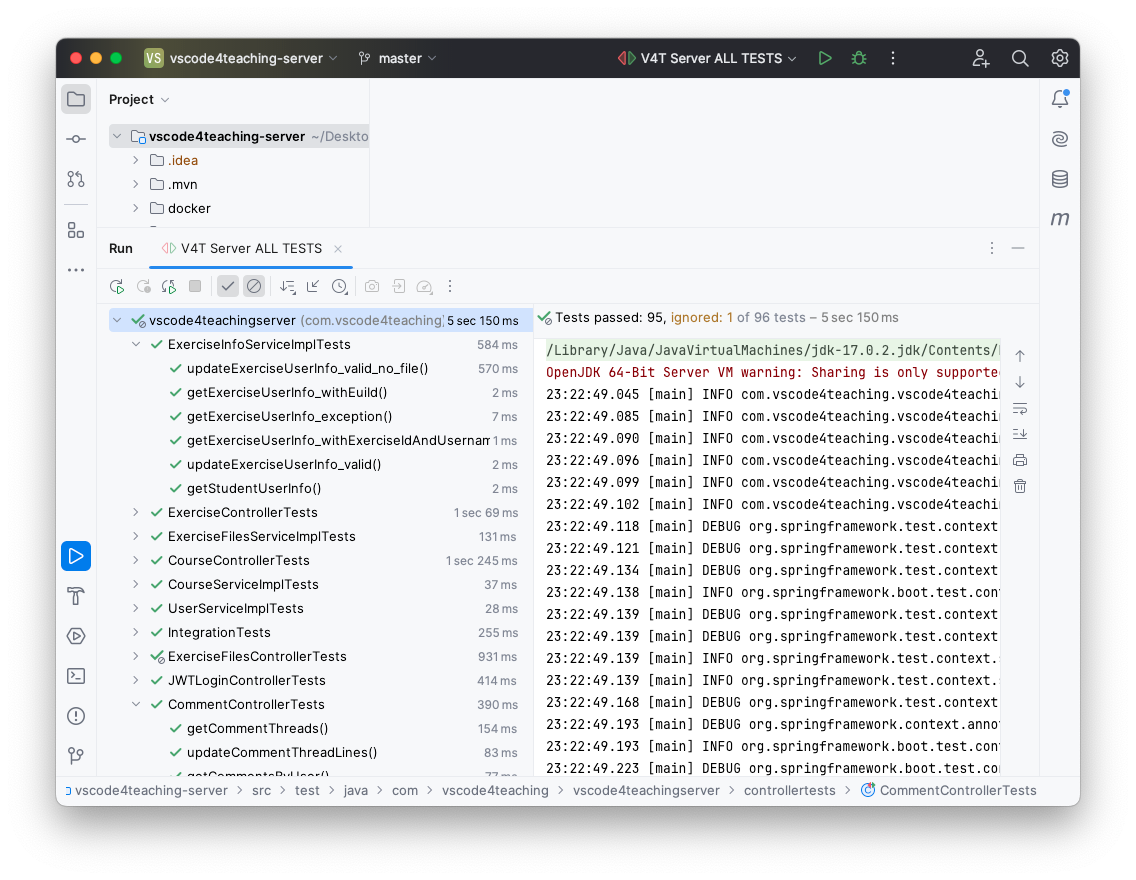
\includegraphics[width=\textwidth]{imagenes/utilizadas/4-4-verificacion/testsServidor.png}
    \caption{Instantánea de \textit{IntelliJ IDEA} mostrando el resultado satisfactorio de la ejecución de las pruebas del servidor.}
    \label{fig:testsServidorIDE}
\end{figure}

Una de las métricas aplicables para valorar la idoneidad o adecuación de las pruebas implementadas al componente realizado es la cobertura del código, que refleja en formato porcentual cuántas líneas o bloques de código han sido revisados por alguna de las pruebas automáticas ejecutadas. En la \referenciaFigura{fig:coberturaServidorFinal} se puede visualizar el informe de cobertura elaborado para el servidor en el momento de la finalización del trabajo. Para este componente, la cobertura de código es del 78,3\% de las clases, el 79,4\% de los métodos y el 77,6\% de las 1180 líneas de código que lo conforman; tasas elevadas que, pese al incremento en el tamaño del componente, permanecen en el mismo orden que al comienzo del proyecto.

\begin{figure}[ht]
    \centering
    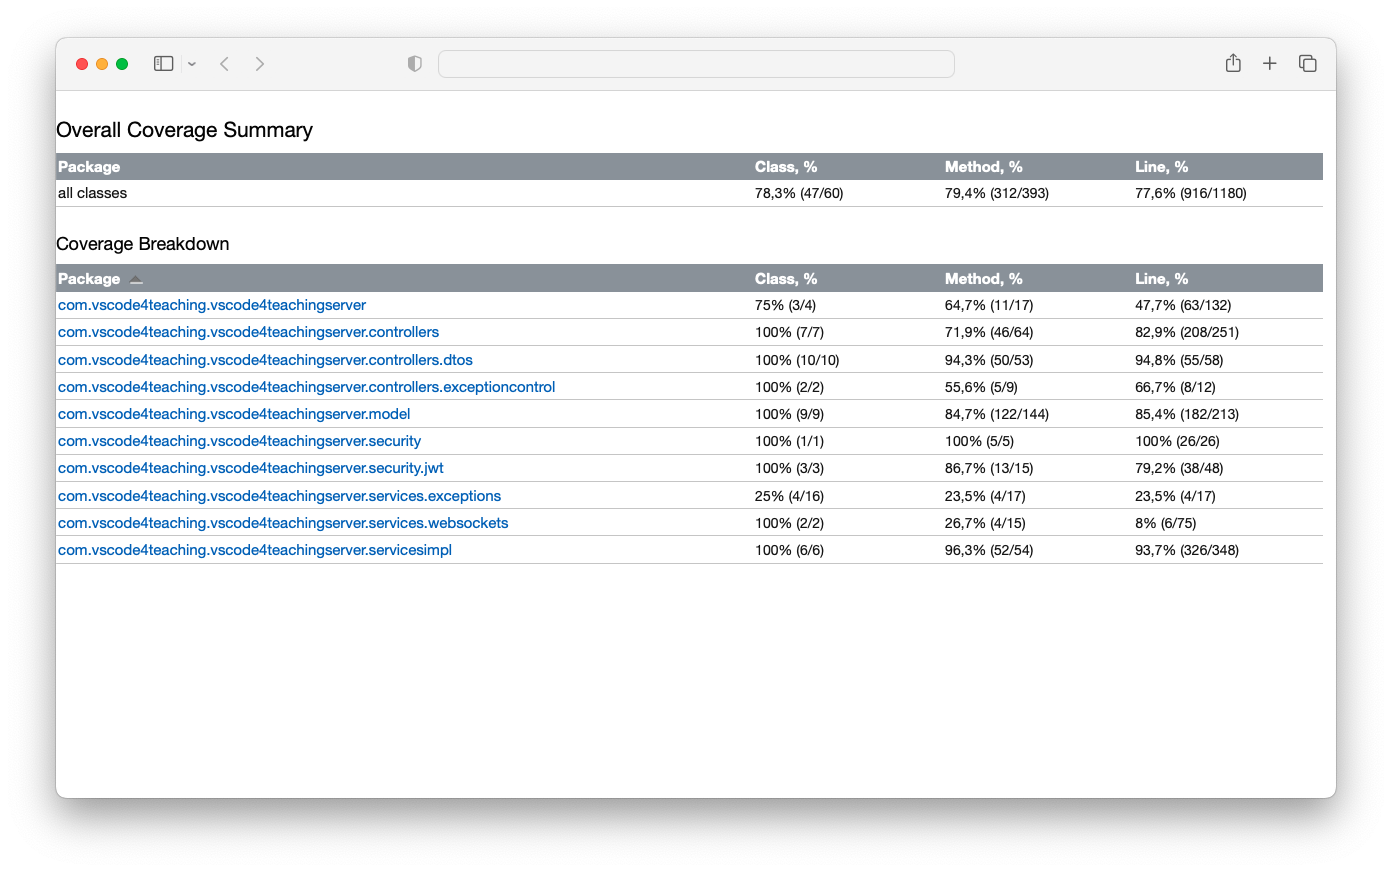
\includegraphics[width=\textwidth]{imagenes/utilizadas/4-4-verificacion/coverageServidorFinal.png}
    \caption{Informe de cobertura de las pruebas automáticas sobre el código del servidor.}
    \label{fig:coberturaServidorFinal}
\end{figure}

\subsubsection{\textit{Testing} de la extensión}
Análogamente al caso anterior, y tal como queda plasmado en la \referenciaSeccion{subsec:tecCliente}, la extensión emplea \textbf{Jest} como librería para la implementación de los \textit{tests} de este componente.

Previamente al inicio de la ejecución de los requisitos comprendidos en el presente Trabajo Fin de Grado, el proyecto contaba con un total de 97 \textit{tests} implementados, alcanzando la cifra de 129 pruebas en el momento de su finalización. La \referenciaFigura{fig:testsClienteIDE} incluye una visualización del entorno de desarrollo una vez terminada la ejecución exitosa de las pruebas implementadas en este componente.

\begin{figure}[ht]
    \centering
    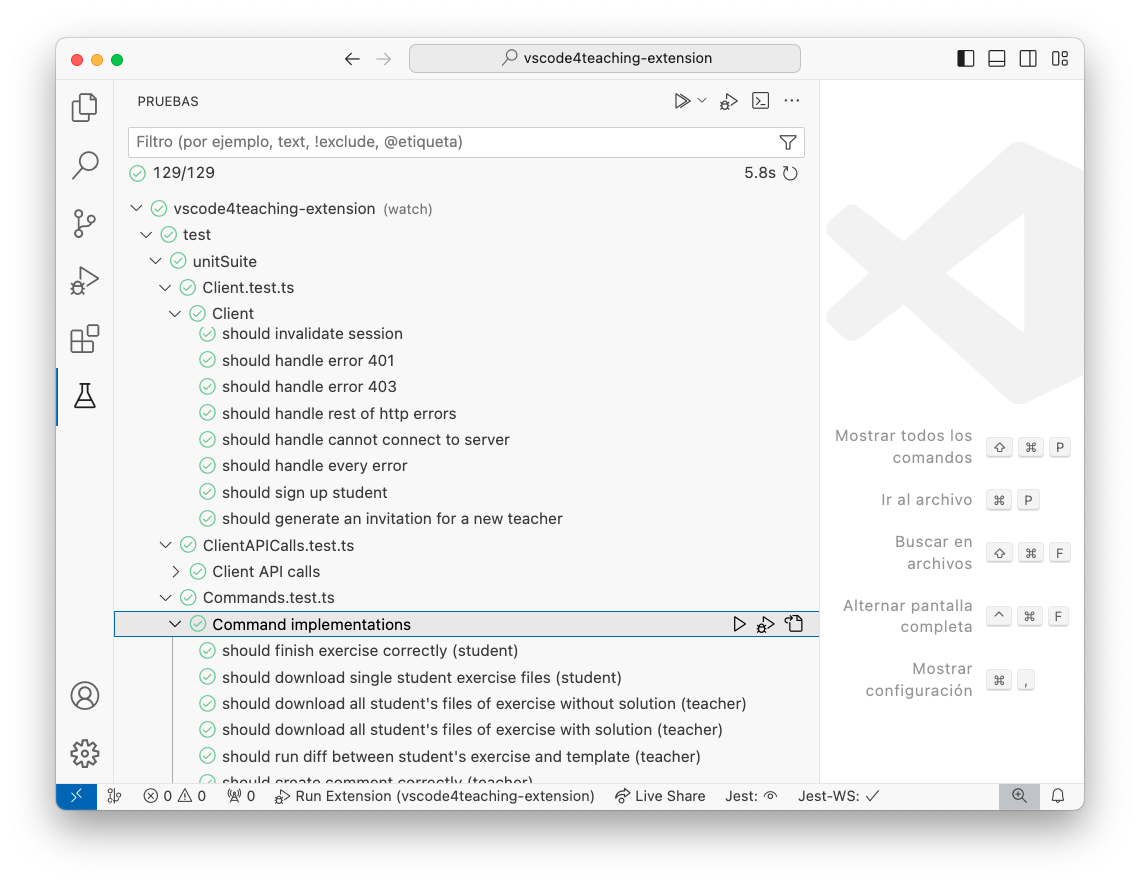
\includegraphics[width=\textwidth]{imagenes/utilizadas/4-4-verificacion/testsCliente.png}
    \caption{Captura de Visual Studio Code tras ejecutar las pruebas implementadas sobre la extensión.}
    \label{fig:testsClienteIDE}
\end{figure}

La \referenciaFigura{fig:coberturaExtensionFinal} introduce el informe de cobertura correspondiente a la extensión en el momento de la finalización del trabajo. En este punto, la cobertura alcanza cifras del 52,08\% de las funciones y el 60,1\% de las 1649 líneas del código generado. Estas tasas se mantienen en el mismo orden que al comienzo del proyecto, poniendo así de manifiesto que se han generado nuevas pruebas para cubrir adecuadamente todos los requisitos implementados y expandido otras anteriormente existentes en el proyecto.

\begin{figure}[ht]
    \centering
    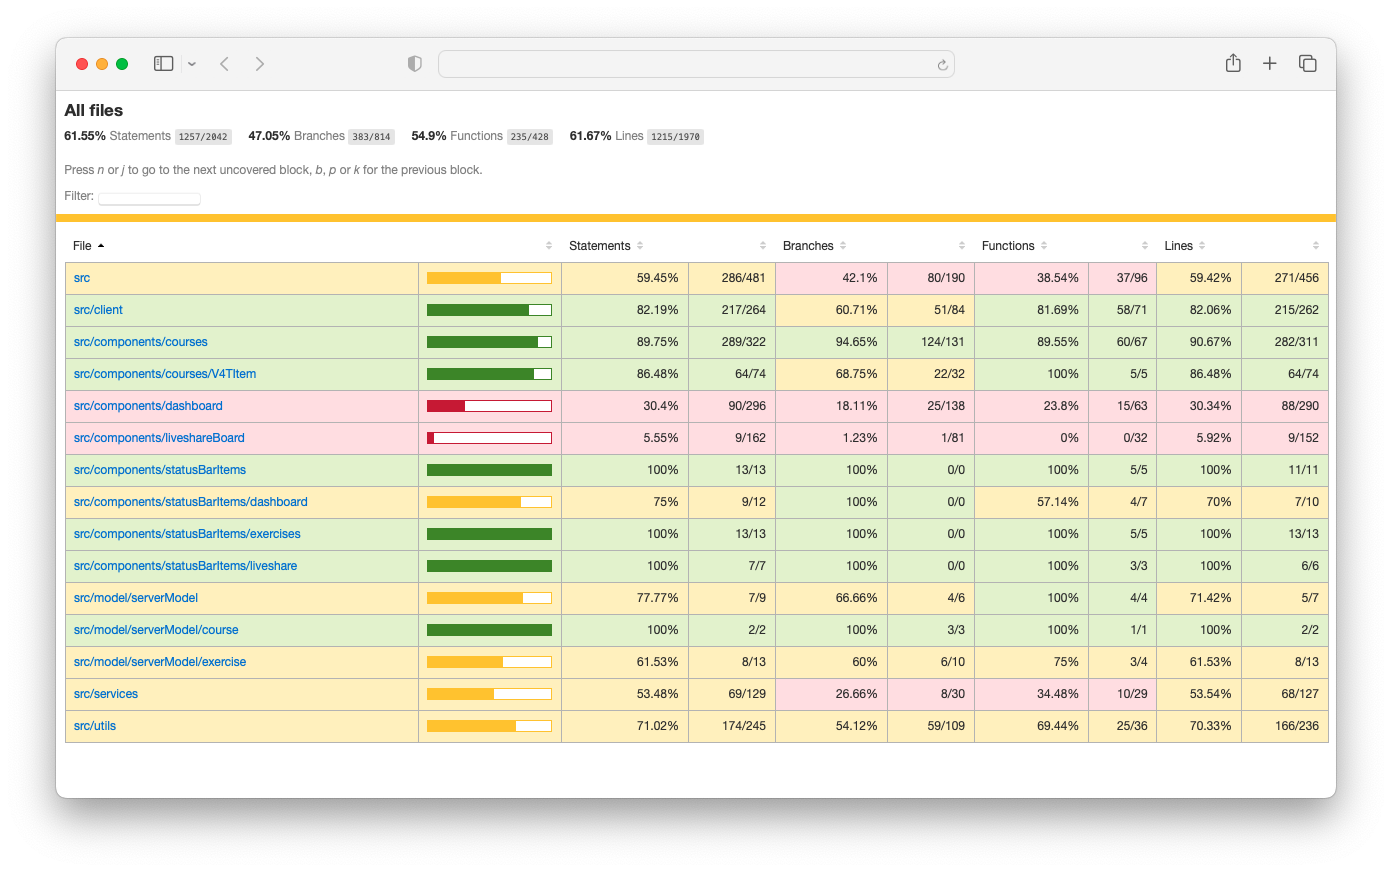
\includegraphics[width=\textwidth]{imagenes/utilizadas/4-4-verificacion/coverageExtensionFinal.png}
    \caption{Informe de cobertura de las pruebas automáticas sobre el código de la extensión para Visual Studio Code.}
    \label{fig:coberturaExtensionFinal}
\end{figure}

\subsection{Pruebas manuales}
\label{subsec:pruebasManuales}
Las pruebas implementadas en código no permiten simular el comportamiento impredecible propio de los usuarios finales de las aplicaciones, de modo que, si bien es posible automatizar pruebas que traten de emular la interacción con el usuario, no es viable fingir un uso real de la aplicación, que se caracterizará por la libertad que estos pueden ejercer en el uso de las funcionalidades de las que dispone el \textit{software} desarrollado.

Para tratar de suplir esta carencia, otro tipo de pruebas realizadas sobre el \textit{software} son las pruebas de \textbf{aceptación de usuario}, en las que una muestra de los usuarios finales acceden a una versión en \textit{pre-producción}, es decir, a una versión que incorpora todas las novedades que se pretende incluir en la nueva evolución del \textit{software} pero divulgada específicamente al grupo acotado de usuarios en régimen de pruebas. De ese modo, los probadores pueden ejecutar una serie de acciones para buscar y detectar errores que puedan escapar a las técnicas de verificación mediante \textit{tests} unitarios o de integración. Adicionalmente, como el proyecto no introduce pruebas de \textbf{rendimiento} o \textbf{carga} automáticas, se aprovecha la ejecución de estas pruebas para evaluar parámetros y detectar errores de estas características.

Durante el presente Trabajo Fin de Grado se han ejecutado pruebas de aceptación de usuario en tres ocasiones, dos de ellas previas al lanzamiento de las versiones más significativas ---véase la \referenciaSeccion{sec:distribDespliegue}--- y una adicional entre las dos anteriores. Las pruebas se han realizado en entornos que simulaban situaciones reales, contando con en torno a cuatro usuarios concurrentes de la extensión que empleaban un mismo servidor de \textit{VSCode4Teaching} desplegado mediante Docker en la red local a la que todos ellos estaban conectados, obteniendo los \textit{logs} registrados de todos los componentes y usuarios para disponer de una traza suficiente para analizar en busca de errores de interacción cliente-servidor en caso de producirse.

La utilidad de este formato de prueba queda confirmada gracias a requisitos de corrección de errores como el \texttt{RE-3} o \texttt{RE-5}, que fueron descubiertos gracias a estas pruebas de aceptación de usuario, permitiendo detectar la fuente del error para proceder con su triaje, tal como se detalla en la \referenciaSeccion{subsec:reqsErrores}. Estas pruebas no solo han servido para detectar y corregir errores: el formato de simulación de entorno real con usuarios potencialmente finales permite obtener realimentación directa del grupo de muestra empleado para introducir requisitos que, bajo su punto de vista, permitan mejorar la usabilidad y comprensibilidad de la aplicación. Prueba de ello es el requisito \texttt{RF-11} ---detallado en la \referenciaSeccion{subsec:rf11}---, por el que se introducen iconos de colores en la barra lateral para expresar información adicional en un solo vistazo, agilizando la interacción del usuario con la aplicación. Estas pruebas han permitido, además, corregir el error asociado al requisito \texttt{RE-6}, por el que se descubrió un problema relativo a la carga de trabajo del servidor, que a menudo era incapaz de procesar todas las peticiones enviadas por los clientes en un mismo instante a la hora de realizar subidas masivas de plantillas y propuestas de resolución de ejercicios por parte de los docentes, tal como queda detallado en la \referenciaSeccion{subsec:reqsErrores}.


% Sección 4.5: Distribución y despliegue
\section{Distribución y despliegue}
\label{sec:distribDespliegue}

La presente sección aborda la forma en que se divulga el código y los recursos asociados al proyecto \textit{VSCode4Teaching}: los canales de distribución del código y de los distintos componentes construidos, así como las distintas versiones lanzadas y distribuidas durante el desarrollo del Trabajo Fin de Grado.

\subsection{Distribución del código fuente}
\textit{VSCode4Teaching} es un proyecto de \textit{software} libre, por lo que puede ser empleado por los usuarios con cualquier fin y su código fuente es público, lo que permite su visualización, modificación y redistribución. Esta permisividad viene estipulada a través de una licencia, que especifica los términos en que se puede emplear el código. La licencia empleada en el proyecto es la Apache License 2.0, que es una licencia permisiva que permite a otros desarrolladores ajenos al proyecto original tomar su código fuente, modificarlo y redistribuirlo libremente siempre que se preserve la licencia a todas aquellas partes que no sean modificadas en las versiones redistribuidas. Se adjunta al proyecto la licencia en el directorio raíz (fichero \texttt{LICENSE}).

El proyecto original queda divulgado a través de un repositorio alojado en el sistema de control de versiones GitHub en el que se puede revisar el crecimiento completo de la aplicación. Es accesible a través de la siguiente dirección:

\vspace{-0.5\baselineskip}
\begin{center}
    \href{https://github.com/codeurjc-students/2019-VSCode4Teaching}{https://github.com/codeurjc-students/2019-VSCode4Teaching}
\end{center}
\vspace{-0.5\baselineskip}

La \referenciaFigura{fig:repoGitHub} muestra la página web del repositorio en GitHub, permitiendo acceder al código fuente de cada uno de los componentes, a la documentación del proyecto en la parte inferior y al histórico de versiones distribuidas a través de la sección ``\textit{Releases}''\footnote{\textit{Release}. Es una versión divulgada de un producto \textit{software} identificada de forma unívoca.} de la barra lateral derecha.

\begin{figure}[ht]
    \centering
    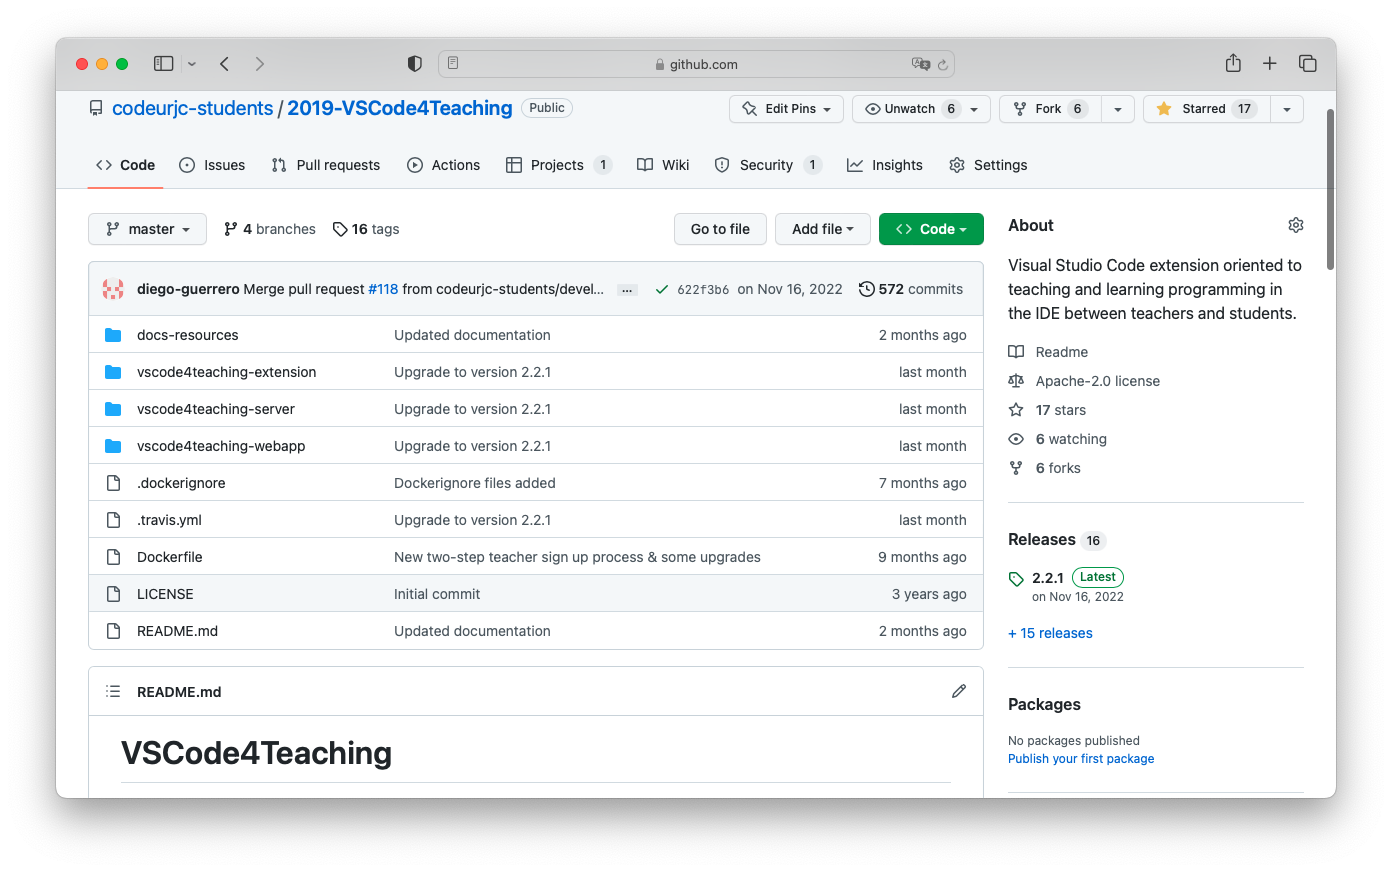
\includegraphics[width=\textwidth]{imagenes/utilizadas/4-5-distribDespliegue/repoGitHub.png}
    \caption{Repositorio de \textit{VSCode4Teaching} en GitHub.}
    \label{fig:repoGitHub}
\end{figure}

\subsection{Versiones de \textit{VSCode4Teaching} publicadas}
El proyecto \textit{VSCode4Teaching} sigue la estrategia de ``versionado semántico'' (del inglés \textit{Semantic Versioning}) \cite{Deploy_SemVer} para la designación de sus versiones. Este formato propone la nomenclatura de las versiones publicadas a través de un identificador con tres números separados por puntos; esto es, con el aspecto \texttt{X.Y.Z}. Sobre este identificador, el número \texttt{Z} aumenta en una unidad cuando la versión únicamente corrige errores menores; el número \texttt{Y}, cuando se añade funcionalidad retrocompatible; y el número \texttt{X}, cuando se introducen cambios no retrocompatibles.

El presente Trabajo Fin de Grado tomó como punto de partida la versión 2.0.2 del proyecto \textit{VSCode4Teaching}. A partir de esta versión, se han divulgado un total de siete nuevas versiones. Las versiones más destacadas publicadas y divulgadas durante el desarrollo del presente trabajo son:
\begin{itemize}
    \item Versión \textbf{2.1.4}. Fue lanzada el 29 de julio de 2022 tras tres versiones previas sobre las que se corrigieron errores. Esta versión introdujo las implementaciones de los requisitos \referenciaConTT{subsec:rf1}{RF-1}, \referenciaConTT{subsec:rf2}{RF-2}, \referenciaConTT{subsec:rf3}{RF-3}, \referenciaConTT{subsec:rf4}{RF-4}, \referenciaConTT{subsec:rf9}{RF-9}, \referenciaConTT{subsec:rf10}{RF-10} y la ejecución al menos una vez de todos los requisitos no funcionales. Se puede acceder al código de esta versión en el repositorio de GitHub a través del enlace:
    \vspace{-0.25\baselineskip}
    \begin{center}
        \href{https://github.com/codeurjc-students/2019-VSCode4Teaching/releases/tag/2.1.4}{https://github.com/codeurjc-students/2019-VSCode4Teaching/releases/tag/2.1.4}
    \end{center}
    \vspace{-0.25\baselineskip}

    \item Versión \textbf{2.2.0}. Fue lanzada el 30 de octubre de 2022, e incorporó como novedades la implementación de los requisitos \referenciaConTT{subsec:rf5}{RF-5}, \referenciaConTT{subsec:rf6}{RF-6}, \referenciaConTT{subsec:rf7}{RF-7}, \referenciaConTT{subsec:rf8}{RF-8}, \referenciaConTT{subsec:rf11}{RF-11} y \referenciaConTT{subsec:rf12}{RF-12}; y una nueva ejecución de los requisitos \referenciaConTT{subsec:rn1}{RN-1} y \referenciaConTT{subsec:rn4}{RN-4}. Análogamente, se puede visualizar en GitHub esta versión accediendo al enlace siguiente:
    \vspace{-0.5\baselineskip}
    \begin{center}
        \href{https://github.com/codeurjc-students/2019-VSCode4Teaching/releases/tag/2.2.0}{https://github.com/codeurjc-students/2019-VSCode4Teaching/releases/tag/2.2.0}
    \end{center}
    \vspace{-0.5\baselineskip}

    Esta versión se vio complementada por la \textbf{2.2.1}, lanzada el 16 de noviembre de 2022, incorporando modificaciones en las dependencias en cumplimiento del requisito \referenciaConTT{subsec:rn1}{RN-1}.
\end{itemize}

% Adicionalmente, se pueden visualizar registros de los cambios incorporados en cada versión de las anteriormente destacadas en el \textit{blog} mantenido durante el transcurso del Trabajo Fin de Grado, accesible a través del siguiente enlace:
% \vspace{-0.5\baselineskip}
% \begin{center}
%     \href{https://medium.com/@diego-guerrero}{https://medium.com/@diego-guerrero}
% \end{center}
% \vspace{-0.5\baselineskip}

\subsection{Despliegue y distribución del servidor}
Tal como se recoge en la \referenciaSeccion{subsec:tecDistribDespliegue}, Docker es una tecnología que facilita los procesos de despliegue y distribución del \textit{software}, ya que permite generar imágenes de programas multiplataforma; esto es, que pueden ser instanciadas como contenedores en cualquier computador con sistemas operativos Windows, macOS o en cualquier distribución de Linux.

El servidor y aplicación web disponen de la configuración adecuada para generar una imagen Docker que permita acceder al servidor (tal como se estipula en el requisito \texttt{RN-3}, desarrollado en la \referenciaSeccion{subsec:rn3}), introduciendo en él previamente durante el proceso de compilación la aplicación web Angular construida en forma de página construida. Esta configuración se introduce en el fichero \texttt{Dockerfile} presente en el directorio raíz.

Una de las formas más sencillas disponible para desplegar una instancia del servidor de \textit{VSCode4Teaching} es hacer uso de la configuración de \textit{Docker Compose} ---tecnología descrita en la sección anteriormente referenciada---, desarrollada e introducida dentro de la implementación del componente servidor (fichero \texttt{docker-compose.yml}).

Una de las posibilidades que Docker brinda a la comunidad de desarrolladores es la de divulgar las imágenes generadas en un repositorio en Internet, Docker Hub, que es una forma simple de ``crear, gestionar y desplegar las aplicaciones [...] en contenedores'' \cite{Deploy_DockerHub}. El servidor, construido tal como se especifica en el \texttt{Dockerfile}, se encuentra publicado en Docker Hub con el nombre \texttt{vscode4teaching/vscode4teaching}. La apariencia de la página de \textit{VSCode4Teaching} en Docker Hub se muestra en la \referenciaFigura{fig:distrib1}, y es accesible en navegadores web a través del enlace:
\vspace{-0.5\baselineskip}
\begin{center}
    \href{https://hub.docker.com/r/vscode4teaching/vscode4teaching}{https://hub.docker.com/r/vscode4teaching/vscode4teaching}.
\end{center}
\vspace{-0.5\baselineskip}

\begin{figure}[ht]
    \centering
    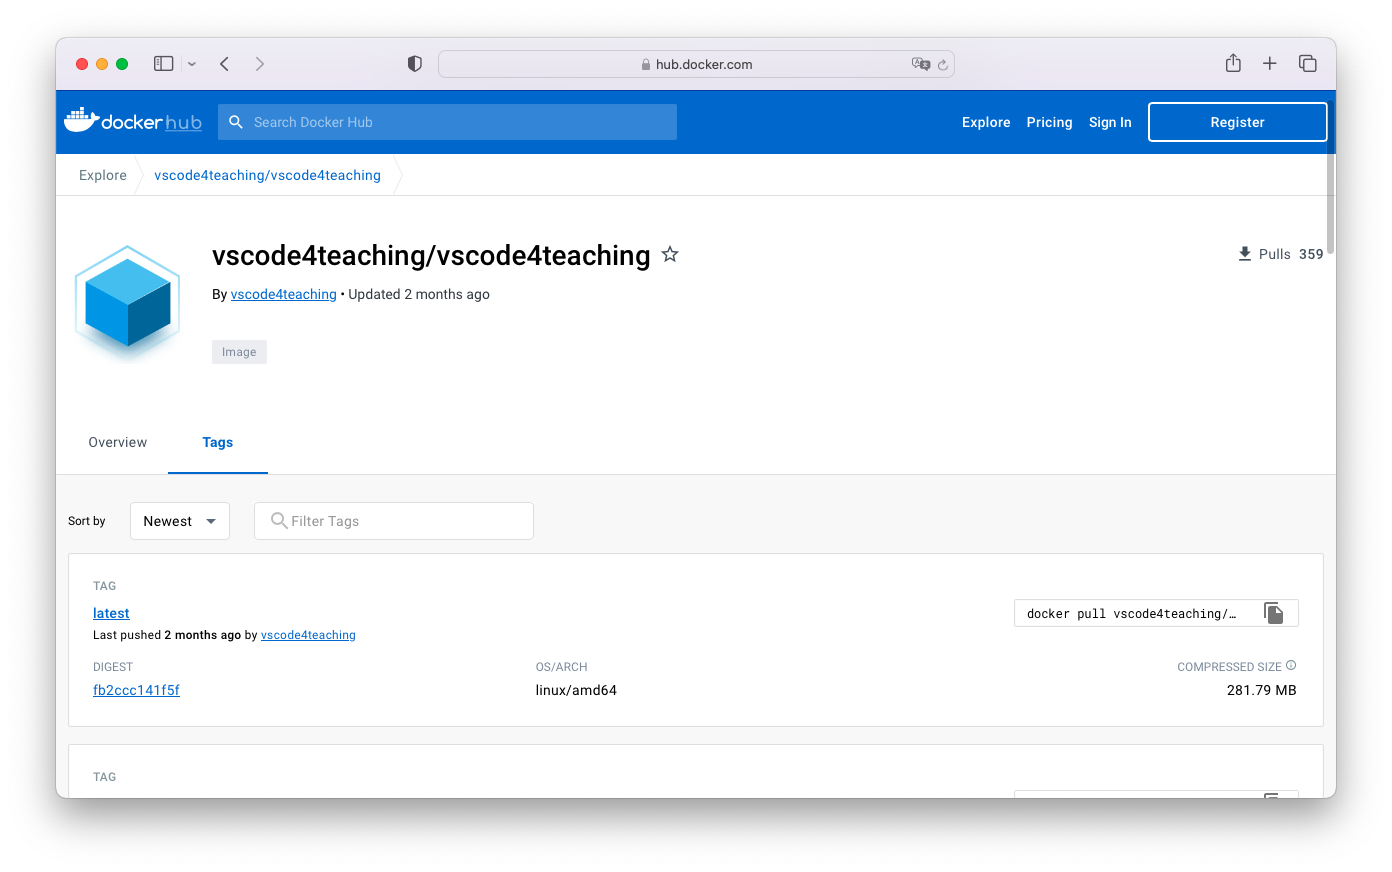
\includegraphics[width=\textwidth]{imagenes/utilizadas/4-5-distribDespliegue/capturaDockerHub.png}
    \caption{Apariencia de la página de \textit{VSCode4Teaching} en Docker Hub.}
    \label{fig:distrib1}
\end{figure}

\subsection{Distribución de la extensión}
Uno de los métodos para la divulgación de extensiones para Visual Studio Code es el \textit{Marketplace}, que es un repositorio que se pone a disposición de los desarrolladores registrados y que permite que ``otros puedan buscar, descargar y utilizar la extensión'' \cite{Tec_VSCPublish}, de modo que cualquier usuario puede descargarla directamente desde el propio entorno de desarrollo o a través de la web, tal como se puede ver en la \referenciaFigura{fig:distrib2}. La extensión ha sido publicada con el nombre \textit{VS Code 4 Teaching}, y se puede visualizar su página de información y descargar a través del enlace:
\vspace{-0.5\baselineskip}
\begin{center}
    \href{https://marketplace.visualstudio.com/items?itemName=VSCode4Teaching.vscode4teaching}{https://marketplace.visualstudio.com/items \\ ?itemName=VSCode4Teaching.vscode4teaching}.
\end{center}
\vspace{-0.5\baselineskip}


\begin{figure}[ht]
    \centering
    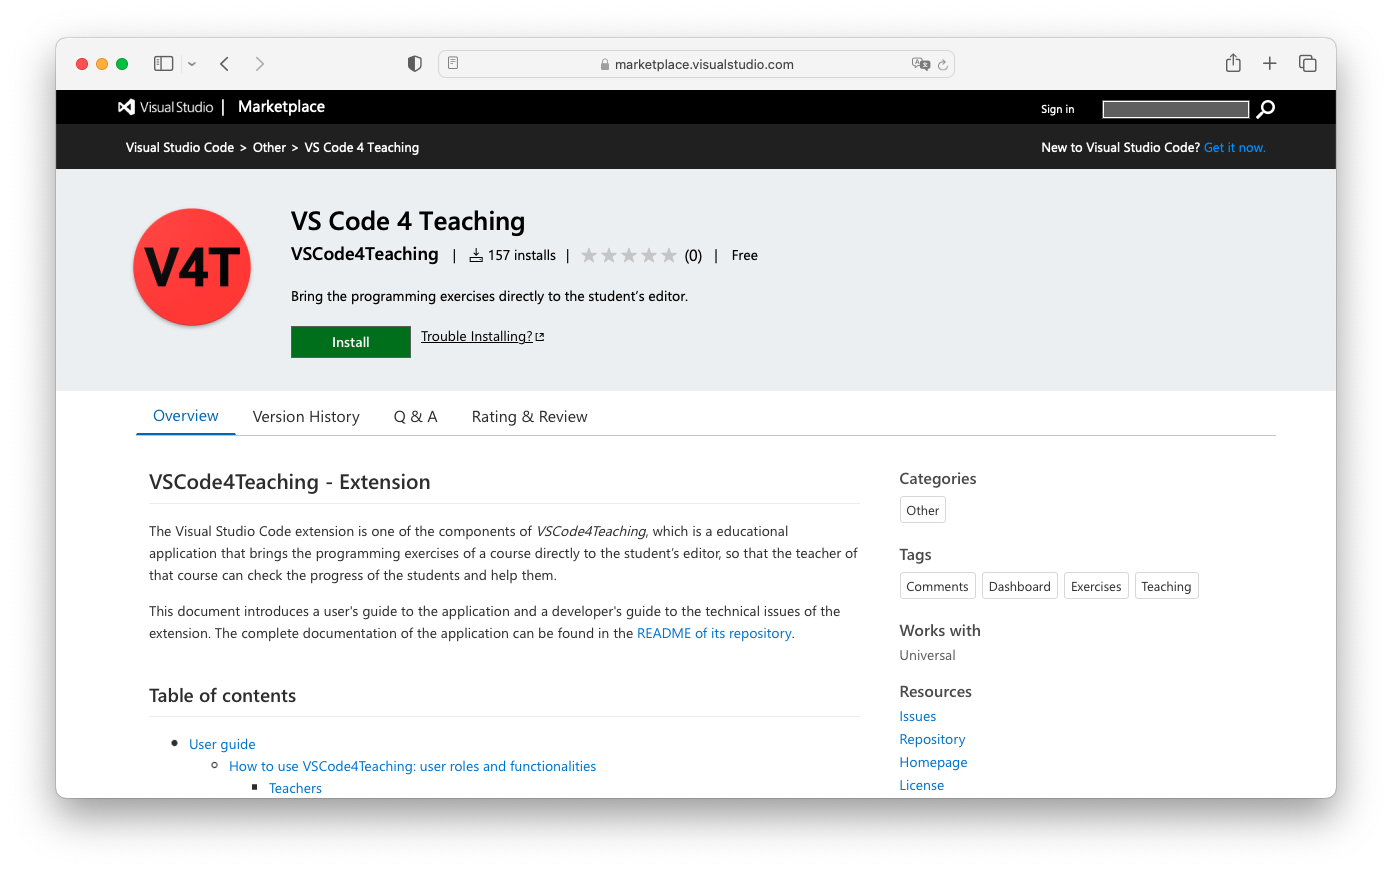
\includegraphics[width=\textwidth]{imagenes/utilizadas/4-5-distribDespliegue/capturaVSCodeMarketplace.png}
    \caption{Apariencia de \textit{VSCode4Teaching} en el \textit{Marketplace} de Visual Studio Code.}
    \label{fig:distrib2}
\end{figure}




% Sección 5: Conclusiones y trabajos futuros.

% Reflexión sobre el trabajo realizado, qué objetivos se han cumpliado y qué aspectos quedan pendientes para una
% futura ampliación del proyecto. Además se deben incluir unas conclusiones personales indicando lo que ha supuesto
% para el alumno la realización del trabajo.
% Extensión recomendada: entre 2 y 4 páginas.
\afterpage{\blankpage}
\chapter{Conclusiones y trabajos futuros}
\label{cap:conclusiones}

Esta sección, última del presente documento, recoge las conclusiones extraídas acerca del trabajo realizado, revisando el cumplimiento de los objetivos estipulados ---\referenciaSeccion{subsec:cumplimientoObjetivos}---, analizando los potenciales trabajos futuros y nuevos objetivos existentes en el proyecto \textit{VSCode4Teaching} ---\referenciaSeccion{subsec:trabajosFuturos}--- e introduciendo una opinión final acerca del transcurso del Trabajo Fin de Grado ---\referenciaSeccion{subsec:aprendizajesPersonales}---.

\section{Cumplimiento de los objetivos estipulados}
\label{subsec:cumplimientoObjetivos}
Respecto a los objetivos del Trabajo Fin de Grado, que quedaron establecidos en el \referenciaCapitulo{cap:objetivos}, y considerando los requisitos especificados en la \referenciaSeccion{sec:requisitos} y desarrollados en las subsiguientes secciones, se constata el cumplimiento de la totalidad de los objetivos prefijados, tal como se desarrolla a continuación:
% . Se revisitan a continuación estos objetivos y se asocia su cumplimiento a los requisitos ejecutados con este fin:
\begin{enumerate}
    \item El objetivo primero establece la necesidad de anonimato de los estudiantes frente al profesorado, requiriendo una modificación del sistema de almacenamiento y la generación de una nueva función que permitiese a los docentes escoger cuándo poder visualizar o no las identidades de sus estudiantes a conveniencia (\referenciaConTT{subsec:rf3}{RF-3}).
    \item El segundo objetivo especifica algunas mejoras acerca de la interacción del profesorado con la aplicación mediante novedades como el sistema de invitación a nuevos docentes (\referenciaConTT{subsec:rf1}{RF-1}) o la posibilidad de añadir varios ejercicios en una única ejecución de un proceso de negocio (\referenciaConTT{subsec:rf2}{RF-2}).
    \item El tercer objetivo estipula la adición de la capacidad para incluir propuestas de soluciones del profesorado en los ejercicios creados. Para ello, se establece que los docentes deben poder añadir soluciones (\referenciaConTT{subsec:rf5}{RF-5}) y controlar, además, cuándo esta solución está disponible a los estudiantes o si pueden continuar editando los ejercicios una vez descargada la solución (\referenciaConTT{subsec:rf6}{RF-6}). Por otro lado, estudiantes y profesores deben poder descargar esta solución, aunque para los estudiantes es preciso controlar que esté disponible (\referenciaConTT{subsec:rf7}{RF-7}). Estos pueden, además, una vez descargada, visualizar fácilmente las diferencias que existan entre ella y su propia propuesta de resolución (\referenciaConTT{subsec:rf8}{RF-8}).
    \item El objetivo cuarto marca la necesidad de potenciar la interacción de los usuarios con la aplicación y se vertebra en dos ejes principales: la necesidad de potenciar la GUI para obtener una apariencia que permita alcanzar una mayor fluidez en el uso de la aplicación y en la introducción de mecanismos de ayuda personalizados para cada usuario con el fin de proporcionar una asistencia eficaz en la utilización de la extensión. En este sentido, se observa el cumplimiento de ambos puntos de la siguiente forma:
    \begin{itemize}
        \item Para mejorar la interfaz de usuario, se introducen modificaciones como: el rediseño integral del \textit{dashboard}, dotándole de una nueva disposición gráfica de elementos y de mayor cantidad de datos actualizados en tiempo real para aportar mejor información al docente (\referenciaConTT{subsec:rf12}{RF-12}); añadiendo, además, la posibilidad de que los docentes previsualicen el \textit{dashboard} de un ejercicio sin necesidad de descargar todos sus ficheros asociados (\referenciaConTT{subsec:rf4}{RF-4}); la incorporación de iconos de colores a la barra lateral para estudiantes y profesores, mostrando más información sobre el estado de cada ejercicio en un solo golpe de vista (\referenciaConTT{subsec:rf11}{RF-11}); y la introducción de un menú contextual ejecutable sobre los cursos para facilitar la ejecución de sus procesos de negocio asociados mediante descripciones textuales aclaratorias, además de mediante los iconos disponibles (\referenciaConTT{subsec:rf10}{RF-10}).
        \item Para proporcionar nuevos mecanismos de ayuda personalizados, se han ejecutado dos actuaciones: la creación de una nueva página de ayuda para estudiantes, facilitando el proceso de inscripción en los cursos mediante explicaciones basadas en el uso de imágenes animadas (\referenciaConTT{subsec:rf9}{RF-9}) y, además, la incorporación de un mecanismo de ayuda rápida en el nuevo \textit{dashboard} para profesores (\referenciaConTT{subsec:rf12}{RF-12}).
    \end{itemize}
    \item El objetivo quinto sitúa la seguridad informática como uno de los pilares fundamentales de esta aplicación. En consonancia con este hecho, se ha ejecutado en varias ocasiones el requisito \referenciaConTT{subsec:rn1}{RN-1} para subsanar las diversas vulnerabilidades aparecidas durante el desarrollo. Además, otros requisitos como el \referenciaConTT{subsec:rf1}{RF-1}, acerca de la reingeniería del proceso para la invitación de nuevos docentes, o algunos de los errores corregidos, analizados en la \referenciaSeccion{subsec:reqsErrores}, eliminan posibles riesgos de seguridad, tales como el \texttt{RE-5}.
    \item El sexto objetivo atribuye una importancia crucial a la detección y corrección de errores durante el proceso de desarrollo o las pruebas en entornos reales. Como consecuencia de la labor de triaje y eliminación de errores surgen todos los requisitos en materia de corrección de errores que se desarrollan en la \referenciaSeccion{subsec:reqsErrores}. Esta labor resulta más sencilla gracias a la ejecución del requisito \referenciaConTT{subsec:rn2}{RN-2}, por el que se han mejorado los sistemas de registro de eventos en todos los componentes de la aplicación, facilitando así el análisis de su comportamiento y las interacciones existentes entre ellos.
    \item El séptimo y último objetivo establece la necesidad de preservar o mejorar la calidad del \textit{software} y atributos relacionados como, por ejemplo, la mantenibilidad. Para ejecutar este objetivo, se han introducido algunas mejoras en el despliegue del servidor (\referenciaConTT{subsec:rn3}{RN-3}) y el requisito \texttt{RN-5}, por el que se ha analizado el código del servidor y la extensión, eliminando duplicidades de código y documentando los procedimientos y algoritmos más complejos.
\end{enumerate}

\section{Trabajos futuros: continuación del proyecto}
\label{subsec:trabajosFuturos}
La realización del trabajo de evolución y mantenimiento analizado en las secciones precedentes ha permitido a las personas involucradas en la concepción y el desarrollo del proyecto \textit{VSCode4Teaching} detectar varias necesidades o potenciales requisitos de interés para su implementación en posteriores etapas del desarrollo.

Entre estas necesidades, la más destacada es la constatación de que muchos estudiantes prefieren utilizar otros entornos de desarrollo distintos de Visual Studio Code, tal como confirma la \textit{Encuesta sobre el Ecosistema de los Desarrolladores} realizada por JetBrains en su edición de 2021 \cite{Conc_EncuestaJetBrains}. Esta encuesta recoge datos sobre los hábitos en torno a la programación de $32\ 570$ desarrolladores, de los que $4567$ afirman ser estudiantes de esta disciplina. Poniendo el foco en este grupo, se obtienen las cifras de uso de IDE que se reflejan en la \referenciaTabla{tab:usoIDEs}. Esta tabla, que refleja cuántos estudiantes utilizan cada uno de los entornos de desarrollo que muestra ---pudiendo cada uno contestar tantos como utilice---, permite observar que Visual Studio Code es el entorno de desarrollo integrado más empleado por los estudiantes de programación, ya que algo más del 53\% de los estudiantes lo utilizan. Sin embargo, son reseñables también las cifras de uso de los entornos de JetBrains, especialmente IntelliJ IDEA y PyCharm, que alcanzan cuotas de uso de alrededor del 39\% y 32\% del estudiantado encuestado, respectivamente.

\begin{table}
    \caption{Adopción de los distintos entornos de desarrollo integrados por los estudiantes encuestados.}
    \label{tab:usoIDEs}
    \centering
    \begin{tabular}{|c|c|c|}
        \textbf{Entorno}   & \textbf{Nº estudiantes} & \textbf{Proporción} \\
        \hline
        Visual Studio Code & 2437                    & 53,36 \%            \\
        \hline
        IntelliJ IDEA      & 1771                    & 38,78 \%            \\
        \hline
        PyCharm            & 1458                    & 31,92 \%            \\
        \hline
        Visual Studio      & 1112                    & 24,35 \%            \\
        \hline
        Android Studio     & 956                     & 20,93 \%            \\
        \hline
        Notepad++          & 685                     & 15,00 \%            \\
        \hline
        Sublime Text       & 637                     & 13,95 \%            \\
        \hline
        CLion              & 565                     & 12,37 \%            \\
        \hline \hline
        Total              & 4567                    &                     \\
        \hline
    \end{tabular}
\end{table}


Como consecuencia de este hecho, se establece como primer y principal trabajo a futuro ejecutar una reorientación del proyecto con el fin de generar una herramienta distinta a la extensión de Visual Studio Code que permita alcanzar la independencia del entorno de desarrollo integrado y que cuente con las mismas o similares funcionalidades que la actual versión, reseñando como piedra angular de la herramienta su capacidad para el seguimiento en tiempo real de la modificación de ficheros locales, de modo que estudiantes y profesores puedan emplear el entorno de desarrollo de su preferencia, emulando las características de las que dispone actualmente con una herramienta independiente del IDE.

Este nuevo trabajo a futuro se suma a los que forman parte de la hoja de ruta del proyecto \textit{VSCode4Teaching}, entre los que cabe destacar los siguientes:
\begin{itemize}
    \item Añadir la capacidad de calificar las propuestas enviadas por los estudiantes para resolver los ejercicios y permitir al alumnado revisar las calificaciones otorgadas, que pueden ser introducidas de forma manual o calculadas automáticamente mediante estrategias para la detección de plagio.
    \item Modificar el sistema de transmisión de las propuestas de resolución de los estudiantes para basarlo en una estrategia de peticiones pequeñas en cada cambio y no en el envío de la propuesta del estudiante completa en cambio para potenciar la eficiencia de la comunicación entre cliente y servidor.
    \item Añadir un rol nuevo para administradores y dotarles de la capacidad para la gestión integral de los usuarios registrados ---estudiantes y profesores--- y los cursos y ejercicios que los componen.
    \item Incorporar nuevas capacidades en torno a los ejercicios, tales como poder fijar fechas de finalización para cada uno o determinar el tiempo máximo disponible para que los estudiantes lo finalicen una vez comenzado.
    \item Integrar la aplicación con entornos Moodle \cite{Moodle} y, específicamente, con el Aula Virtual de la Universidad Rey Juan Carlos mediante el uso de un interfaz LTI\footnote{LTI. Siglas de ``interoperabilidad entre herramientas de aprendizaje'' (del inglés \textit{Learning Tools Interoperability}).} \cite{LTI_Spec}.
\end{itemize}

\section{Aprendizajes personales}
\label{subsec:aprendizajesPersonales}
Me tomo la licencia de redactar en primera persona la sección que cierra esta memoria de mi primer Trabajo Fin de Grado, en la que recopilo las conclusiones personales que aprendo tras esta experiencia.

Mi doble grado ha sido, en mi opinión, un conjunto de más de treinta asignaturas con un marcado carácter teórico y, al menos hasta el tercer curso, han tenido la intención principal de inculcar las bases y principios sobre los que se asienta la informática tal como es entendida en la actualidad. Si bien a partir del tercer curso las asignaturas empiezan a tomar un carácter práctico algo más cercano a la futura realidad laboral que la Universidad busca preparar, este Trabajo Fin de Grado ha sido mi primera oportunidad para ``aterrizar'' todos los conocimientos aprendidos durante el transcurso de la carrera en el contexto de un proyecto real.

Una de las mayores lecciones que aprendo es que la evolución y adaptación del \textit{software} es una de las tareas más complejas que hay en la ingeniería del \textit{software}. Son pocos los proyectos que se arrancan desde cero en un contexto en el que la informática lleva ya al menos veinte años copando todas las áreas y formando parte de la inmensa mayoría de los procesos de negocio existentes, lo que hace que, tal como he tenido oportunidad de ratificar en mi experiencia laboral, muchos de los requisitos necesarios se implementen en proyectos ya existentes previamente. Indudablemente, la tarea más compleja que he ejecutado en este Trabajo Fin de Grado ha sido entender qué se había implementado cuando yo llegué, cómo se había diseñado la herramienta, cómo funcionaban las tecnologías sobre las que se asentaba y de qué manera podría ``abrir'' el código sobre mi ``mesa de operaciones'' para comenzar a implementar los nuevos requisitos que aspirábamos a introducir en el proyecto.

Una vez vencida esta dificultad, este TFG me ha permitido asentar los conocimientos de muchas asignaturas, especialmente de aquellas que versan sobre la ingeniería del \textit{software} en sí misma ---con una especial mención a Evolución y Adaptación del \textit{Software}---, las que enseñan acerca del desarrollo web ---con otra especial mención a Desarrollo de Aplicaciones Web--- y, además, todas las asignaturas ``básicas'' sobre programación, orientación a objetos o redes de computadores, que subyacen debajo de las primeras. Además, me ha permitido acercarme a áreas que había explorado poco, que he utilizado más en el ámbito laboral desde entonces y de las que quiero seguir aprendiendo, como son la computación en la nube, con el enorme potencial que hay detrás de Docker, o el conjunto de prácticas que integran \textit{DevOps}, con especial interés por las buenas prácticas en integración, despliegue y entrega continuos.

Con todos estos aprendizajes, \textit{VSCode4Teaching} continuará creciendo en mi segundo Trabajo Fin de Grado.

%%%%%%%%%%%%%%%%%%%%%%%%%%%%%%% Bibliografía %%%%%%%%%%%%%%%%%%%%%%%%%%%%%%%
\afterpage{\blankpage}
\renewcommand{\bibname}{Bibliografía}
\phantomsection
\begin{thebibliography}{99}
    \addcontentsline{toc}{chapter}{Bibliografía}
    % 1. Introducción
    \bibitem{INEMyH2021} Instituto Nacional de Estadística. (Diciembre de 2021). \textit{Mujeres y hombres en España}, Secciones 6.5 y 6.6. \href{https://www.ine.es/ss/Satellite?L=es_ES&c=INEPublicacion_C&cid=1259924822888&p=1254735110672&pagename=ProductosYServicios%2FPYSLayout&param1=PYSDetalleGratuitas&param2=1259925527407&param4=Mostrar}{https://ine.es}.
    \bibitem{BOEMEFP2022} Real Decreto 217/2022, por el que se establece la ordenación y las enseñanzas mínimas de la Educación Secundaria Obligatoria. (29 de marzo de 2022, publicado en BOE núm. 76, de 30 de marzo de 2022, páginas 41571 a 41789). \href{https://www.boe.es/eli/es/rd/2022/03/29/217}{https://boe.es}.
    \bibitem{CMEdu2015} Boletín Oficial de la Comunidad de Madrid. (Mayo de 2015). Decreto 48/2015, de 14 de mayo, por el que se establece para la Comunidad de Madrid el currículo de la Educación Secundaria Obligatoria. (BOCM núm. 118, páginas 10 a 309). \href{https://bocm.es/boletin/bocm-20150520-118}{https://bocm.es}.
    \bibitem{INECOVID_Teletrabajo2020} Instituto Nacional de Estadística. (2021). \textit{Encuesta de condiciones de vida. Módulo 2021.} \href{https://www.ine.es/dynt3/inebase/index.htm?padre=7989&capsel=7989}{https://ine.es}.
    \bibitem{INECOVID_TeletrabajoFeb2020} Instituto Nacional de Estadística. (2020). \textit{El teletrabajo en España y la UE antes de la COVID-19} (publicado en el boletín CifrasINE). \href{https://www.ine.es/ss/Satellite?blobcol=urldata&blobheader=application%2Fpdf&blobheadername1=Content-Disposition&blobheadervalue1=attachment%3B+filename%3Dcfr_022020_v4.pdf&blobkey=urldata&blobtable=MungoBlobs&blobwhere=787%2F725%2Fcfr_022020_v4.pdf&ssbinary=true}{https://ine.es}.
    \bibitem{TFG_Ivan} Chicano Capelo, I. (2020). \textit{VS Code 4 Teaching: Los ejercicios directos al editor}.
    \bibitem{TFG_Alvaro} Rivas Alcobendas, Á. J. (2021). \textit{VSCode4Teaching 2.0: Seguimiento de ejercicios de alumnos en el IDE del profesor}.
    \bibitem{Tec_LiveShare} Microsoft. (2022). \textit{Visual Studio Live Share: Herramienta de colaboración de código en tiempo real}. \href{https://visualstudio.microsoft.com/es/services/live-share/}{https://visualstudio.microsoft.com}.
    \bibitem{Intro_PairProgramming} Agile Alliance. \textit{Pair Programming}. \href{https://www.agilealliance.org/glossary/pairing/#q=~(infinite~false~filters~(postType~(~'page~'post~'aa_book~'aa_event_session~'aa_experience_report~'aa_glossary~'aa_research_paper~'aa_video)~tags~(~'pair*20programming))~searchTerm~'~sort~false~sortDirection~'asc~page~1)}{https://agilealliance.org}.

    % 3.1. Tecnologías
    \bibitem{Tec_MySQL} Oracle Corporation. (2022). \textit{MySQL Community Edition}. \href{https://www.mysql.com/products/community/}{https://mysql.com}.
    \bibitem{Tec_Encuesta_StackOverflow} Stack Overflow. (2021). \textit{Stack Overflow Developer Survey 2021}. \href{https://survey.stackoverflow.co/2021}{https://survey.stackoverflow.co}.
    \bibitem{Tec_Java} Oracle Corporation. (2022). \textit{¿Qué es Java y por qué lo necesito?} \href{https://www.java.com/es/download/help/whatis_java.html}{https://java.com}.
    \bibitem{TIOBE} TIOBE. (1 de noviembre de 2022). \textit{Índice TIOBE}. \href{https://www.tiobe.com/tiobe-index/}{https://tiobe.com}.
    \bibitem{Tec_Maven} The Apache Software Foundation. (2022). \textit{Maven - Welcome to Apache Maven}. \href{https://maven.apache.org}{https://maven.apache.org}.
    \bibitem{Tec_Spring} Broadcom, Inc. (2022). \textit{Spring | Why Spring?} \href{https://spring.io/why-spring}{https://spring.io}.
    \bibitem{Tec_SpringBoot} Spring \& Broadcom, Inc. (2022). \textit{Spring Boot}. \href{https://spring.io/projects/spring-boot}{https://spring.io}.
    \bibitem{Tec_JUnit} JUnit. (2022). \textit{JUnit 5}. \href{https://junit.org/junit5/}{https://junit.org}.
    \bibitem{Tec_Node} OpenJS Foundation. (2022). \textit{Acerca | Node.js}. \href{https://nodejs.org/es/about/}{https://nodejs.org}.
    \bibitem{Tec_NPM} NPM, Inc. (2022). \textit{About npm | npm Docs}. \href{https://docs.npmjs.com/about-npm}{https://docs.npmjs.com}.
    \bibitem{Tec_TS} Microsoft. (2022). \textit{TypeScript: JavaScript with syntax for types}. \href{https://www.typescriptlang.org}{https://typescriptlang.org}.
    \bibitem{Tec_VSCodeExtAPI} Microsoft. (2022). \textit{Extension API | Visual Studio Code Extension API}. \href{https://code.visualstudio.com/api}{https://code.visualstudio.com}.
    \bibitem{Tec_VSCPublish} Microsoft Inc. (2022). \textit{Publishing Extensions | Visual Studio Code Extension API}. \href{https://code.visualstudio.com/api/working-with-extensions/publishing-extension}{https://code.visualstudio.com}.
    \bibitem{Tec_Jest} Open JS Foundation. (2022). \textit{Jest · Delightful JavaScript Testing}. \href{https://jestjs.io/}{https://jestjs.io}.
    \bibitem{Tec_Vue} You, E. (2022). \textit{Vue.js - The Progressive JavaScript Framework}. \href{https://vuejs.org}{https://vuejs.org}.
    \bibitem{Tec_React} Meta Platforms. (2022). \textit{React - Una biblioteca de JavaScript para construir interfaces de usuario}. \href{https://es.reactjs.org}{https://es.reactjs.org}.
    \bibitem{Tec_Angular} Google Inc. (2022). \textit{Angular}. \href{https://angular.io}{https://angular.io}.
    \bibitem{Tec_Docker} Docker Inc. (2022). \textit{Docker: Accelerated, Containerized Application Development}. \href{https://www.docker.com}{https://docker.com}
    \bibitem{Tec_DockerContainers} Docker Inc. (2022). \textit{What is a Container?} \href{https://www.docker.com/resources/what-container/}{https://docker.com}
    \bibitem{Tec_DockerCompose} Docker Inc. (2022). \textit{Docker Compose | Docker Documentation}. \href{https://docs.docker.com/compose/}{https://docker.com}.

    % 3.2. Herramientas
    \bibitem{Her_VSCode} Microsoft. (2022). \textit{Visual Studio Code - Code Editing. Redefined}. \href{https://code.visualstudio.com}{https://code.visualstudio.com}.
    \bibitem{Her_IntelliJ} JetBrains. (2022). \textit{IntelliJ IDEA: el IDE de Java eficaz y ergonómico de JetBrains}. \href{https://www.jetbrains.com/es-es/idea/}{https://jetbrains.com}.
    \bibitem{Her_WebStorm} JetBrains. (2022). \textit{WebStorm: el IDE de JavaScript y TypeScript de JetBrains}. \href{https://www.jetbrains.com/es-es/webstorm/}{https://jetbrains.com}.
    \bibitem{Her_DBeaver} DBeaver. (2022). \textit{DBeaver Community | Free Universal Database Tool}. \href{https://dbeaver.io}{https://dbeaver.io}.
    \bibitem{Her_Git} Software Freedom Conservancy. (2022). \textit{Git}. \href{https://git-scm.com}{https://git-scm.com}.
    \bibitem{Her_GitHub} GitHub Inc. (2022). \textit{GitHub}. \href{https://github.com/about}{https://github.com}.
    \bibitem{Her_DevOps} Atlassian. (2022). \textit{¿Qué es DevOps? | Atlassian}. \href{https://www.atlassian.com/es/devops/}{https://www.atlassian.com}.
    \bibitem{Her_CICD} GitLab. (2022). \textit{What is CI/CD?} \href{https://about.gitlab.com/topics/ci-cd/}{https://about.gitlab.com}.
    \bibitem{Her_Travis} Travis CI GmbH. (2022). \textit{Travis CI - Testing your building blocks}. \href{https://www.travis-ci.com/about-us/}{https://travis-ci.com}.

    \bibitem{Her_Trello} Atlassian. (2022). \textit{Trello}. \href{https://trello.com}{https://trello.com}.

    % 3.3. Metodología
    \bibitem{Met_AgileManifesto} Beck, K., et al. (2001). \textit{Manifesto for Agile Software Development}. \href{https://agilemanifesto.org}{https://agilemanifesto.org}.
    \bibitem{Met_AgileFrameworks} Sylvanns, D. (30 de septiembre de 2022). \textit{7 Different Types Of Agile Methodologies}. \href{https://www.itbriefcase.net/7-different-types-of-Agile-methodologies}{https://itbriefcase.net}.
    \bibitem{Met_TableroKanban} Kanbanize. (2022). \textit{¿Qué es un tablero Kanban y cómo utilizarlo?} \href{https://kanbanize.com/es/recursos-de-kanban/primeros-pasos/que-es-tablero-kanban}{https://kanbanize.com}.

    % 4.1. Requisitos
    \bibitem{XP_UserStories} Sergeev, A. (26 de mayo de 2016). \textit{Extreme programming user stories}. \href{https://hygger.io/blog/extreme-programming-user-stories/}{https://hygger.io}.

    % 4.2. Arquitectura
    \bibitem{IONOSWebSocket} IONOS. (2020). \textit{¿Qué es WebSocket?}. \href{https://www.ionos.es/digitalguide/paginas-web/desarrollo-web/que-es-websocket/}{https://ionos.es}.
    \bibitem{Arq_MVCFowler} Fowler, M. (2002). \textit{Patterns of enterprise application architecture}. Addison-Wesley Professional. \href{https://www.oreilly.com/library/view/patterns-of-enterprise/0321127420/}{https://oreilly.com}.
    % \bibitem{Arq_UncleBob} Martin, R. C. (2018). \textit{Clean architecture} (2ª edición). Addison-Wesley.
    \bibitem{Arq_JWT} Okta Inc. (2022). \textit{JSON Web Token Introduction}. \href{https://jwt.io/introduction}{https://jwt.io}.
    \bibitem{Arq_CSRF} OWASP Foundation. (2022). \textit{Cross Site Request Forgery (CSRF)}. \href{https://owasp.org/www-community/attacks/csrf}{https://owasp.org}.
    \bibitem{Arq_AngularComponents} Google Inc. (2022). \textit{Angular Components overview}. \href{https://angular.io/guide/component-overview}{https://angular.io}.
    \bibitem{Arq_AngularRouter} Google Inc. (2022). \textit{Angular - Router reference}. \href{https://angular.io/guide/router-reference}{https://angular.io}.

    % 4.3. Implementación
    \bibitem{rn1_queEsCiber} Cisco Systems, Inc. (2022). \textit{¿Qué es la ciberseguridad? - Cisco}. \href{https://www.cisco.com/c/es_mx/products/security/what-is-cybersecurity.html}{https://cisco.com}.
    \bibitem{rn1_cve} The MITRE Foundation. (2022). \textit{CVE}. \href{https://www.cve.org}{https://cve.org}.
    \bibitem{rn2_tecLogServidor} The Apache Software Foundation. (2022). \textit{Log4j - Apache Log4j 2}. \href{https://logging.apache.org/log4j/2.x/}{https://apache.org}.
    \bibitem{rn2_tecLogExtension} Robbins, C., Hyde, D et al. (2022). \textit{Winston: A logger for just about everything}. \href{https://github.com/winstonjs/winston}{https://github.com}.
    \bibitem{rn2_tecLogAppWeb} Fannin, D et al. (2021). \textit{Ngx-Logger: Angular logger}. \href{https://github.com/dbfannin/ngx-logger}{https://github.com}.
    \bibitem{rn3_multistage} Docker, Inc. (2022). \textit{Multi-stage Builds | Docker Documentation}. \href{https://docs.docker.com/build/building/multi-stage/}{https://docker.com}.
    \bibitem{rn3_dockerfile} Docker, Inc. (2022). \textit{Dockerfile Reference | Docker Documentation}. \href{https://docs.docker.com/engine/reference/builder/}{https://docker.com}.
    \bibitem{rn4_swagger} SmartBear Software. (2022). \textit{API Documentation \& Design Tools for Teams | Swagger}. \href{https://swagger.io}{https://swagger.io}.
    \bibitem{rn4_openapi} The Linux Foundation. (2022). \textit{OpenAPI Initiative}. \href{https://www.openapis.org}{https://openapis.org}.
    \bibitem{rn4_swaggerui} SmartBear Software. (2022). \textit{REST API Documentation Tool | Swagger UI}. \href{https://swagger.io/tools/swagger-ui/}{https://swagger.io}.

    % 4.5. Despliegue
    \bibitem{Deploy_SemVer} Preston-Werner, T. (2022). \textit{Semantic Versioning 2.0.0}. \href{https://semver.org}{https://semver.org}.
    \bibitem{Deploy_DockerHub} Docker Inc. (2022). \textit{Docker Hub Container Image Library}. \href{https://hub.docker.com}{https://docker.com}.

    % 5. Conclusiones y trabajos futuros
    \bibitem{Conc_EncuestaJetBrains} Sichkarenko, A. (2021, Sep 28). \textit{Developer Ecosystem Survey 2021: Raw data available}. \href{https://blog.jetbrains.com/blog/2021/09/28/developer-ecosystem-survey-2021-raw-data-available/}{https://jetbrains.com}.
    \bibitem{Moodle} Moodle. \textit{Moodle - Open-source learning platform}. \href{https://moodle.org}{https://moodle.org}.
    \bibitem{LTI_Spec} IMS Global Learning Consortium. (16 de abril de 2019). \textit{Learning Tools Interoperability Core Specification} (versión 1.3). \href{https://www.imsglobal.org/spec/lti/v1p3}{https://imsglobal.org}.
\end{thebibliography}

% \afterpage{\blankpage}
% \newpage


%%%%%%%%%%%%%%%%%%%%%%%%%%%%%%% Apéndices %%%%%%%%%%%%%%%%%%%%%%%%%%%%%%%

% \appendix

% \phantomsection
% \addcontentsline{toc}{chapter}{Apéndices}

% \mbox{}
% \vfill
% \begin{center}
% \begin{Huge}
% \textbf{Apéndices}
% \end{Huge}
% \end{center}
% \vfill
% \mbox{}
% \thispagestyle{empty}

% \newpage
% \mbox{}
% \thispagestyle{empty}
% \newpage

% \input{secciones/6-apendices/6-apendices.tex}

% Fin del documento
\end{document}
